\documentclass{xdupgthesis}
\usepackage{amsmath}
\usepackage{geometry}
\usepackage{booktabs}
\usepackage{xcolor}
\usepackage{graphicx}
\usepackage{algorithm}
\usepackage{algorithmic}
\usepackage{anyfontsize} % For precise font size control
\usepackage{array} % For table formatting
% \usepackage[utf8]{inputenc}
% \usepackage[natbib=true, style=apa]{bibentry}
% \nobibliography*
% \setCJKmainfont[Path = fonts/, BoldFont = AdobeFangsongStd-Regular.otf]{AdobeFangsongStd-Regular.otf}

\graphicspath{{AllImagesForUse/}}
\DeclareGraphicsExtensions{.pdf}

\xdusetup{
     style = {
        cjk-font = fandol,
        latin-font = gyre,
        en-cjk-font = true,
        unicode-math = {amsmath},
        page-vertical-align = {分散对齐},
        remove-page= {封面, 题名页, 致谢},
        customize-los = true,
        customize-loa = true
    },
    info = {
        student-id = {22036212602},
        title = {Stock Market Price Forecasting Using\\
        Deep Reinforcement Learning Techniques},
        author = {ABU SAYEM MD HABIBULLAH},
        department = {School of Computer Science and Technology},
        major = {Computer Science and Technology},
        supervisor = {Prof. Wang Shuzhen（王书振）},
        degree = 工程硕士,
        keywords* = {Deep reinforcement learning, stock market prediction, financial time series prediction, algorithmic trading, Bayesian optimization},
        keywords = {深度强化学习, 股市预测, 金融时间序列预测, 算法交易, 贝叶斯优化},
        abstract* = {chapters/abstract.tex},
        abstract = {chapters/abstractcn.tex},
        bib-resource = {
            bib/dl.bib,
            bib/bop.bib,
            bib/findrl.bib,
            bib/stratigies.bib, 
        },
        acknowledgements = {chapters/acknowledgements.tex},
        appendix = {chapters/appendix.tex},
        los = {chapters/symbols.tex},
        loa = {chapters/abbreviation.tex}
    }
}


% Table of Contents, List of Figures, List of Tables
\begin{document}
% \listoffigures
% \listoftables
% \newpage
% \tableofcontents


% Chapter: Introduction
\include{chapters/introduction} 

% Chapter: Litarature Review
% \include{chapters/introduction} 
% \fbox{\includegraphics[width=0.7\textwidth]{performance/unsplash.jpg}}
% Chapter 01:
\chapter{Trading Strategies Architectural Design: A Comparative Analysis of 20 Technical Indicators, Using a Dynamic Backtesting, and Performance Evaluation}

\textbf{Abstract: } 
In this study, we present a broad architectural layout for a trading strategy via comparative analysis of 20 technical indicators—predicated “FinDRL – *”—created in PineScript V6 on the TradingView interface. Each strategy, which we add a Stochastic RSI filter to, incorporates trend-following, breakout, mean-reversion and volume-based approaches. This study is comprehensive and discusses the mathematical theory, the design principles, and implementation methodologies for each strategy, all back-tested dynamically using daily NVIDIA (NVDA, NASDAQ) data over a range of dates (2007–2025).
The 20 strategies were chosen as a result of an extended evaluation of more than 500 strategies over the last 2 years and considering performance robustness and empirical results. The most profitable strategy was FinDRL - Momentum with a net profit +38.62 USD (+0.39\%) at 1,065 trades while FinDRL - Bollinger Bands and FinDRL - Parabolic SAR lost: -0.78 USD and -9.89 USD, respectively. In addition to this, FinDRL – Williams \%R and FinDRL – Volume Spike also provided the highest profit factors (1.972 and 2.469), thus better risk-adjusted return. In contrast, it is worth mentioning that some strategies, such as FinDRL - Donchian Channel, FinDRL - ATR and FinDRL - RSI had no trades, indicating potential backtesting difficulties.
The research presented a unified methodology to formulate and empirically evaluate algorithmic trading strategies through quantitative analysis of historical trading data, adaptive tuning of trading parameters and redoubtable risk management aspects. Following on from these discoveries, work in the Future, “Maximizing Market Returns Optimizing Technical Indicators: A Bayesian Optimization Approach”, will investigate using Bayesian optimization techniques to further optimize indicator parameters and improve trading performance. This study provides further insights for finance practitioners and academic researchers, providing a systematic road map for connecting theoretical design with actionable trading practices.

\section{Introduction}
Technical indicators have been the bedrock of algorithmic trading, providing the mathematical lenses through which we turn historical price and volume data into actionable buy/sell signals. In the current round of frenetic financial markets, these indicators are vital for trend detection, volatility measurement, and potential reversal acceleration. In this study, we propose a full comparison of 20 different trading strategies grouped as “FinDRL – *” based on a Technical Indicator of level built using PineScript V6 on the TradingView platform. Using daily 2007 through 2025 dynamic backtesting for NVIDIA (NVDA, NASDAQ), we have a comprehensive dataset to understand the performance metrics based on net profit, profit factors, drawdowns, and trade frequency.

On a high level, technical indicators are simple mathematical constructs that aggregate raw market data into signals, which then inform trading decisions. A case in point is the Gaussian Channel which utilizes weighted moving averages with Gaussian kernel to generate adaptive support and weighted moving averages with Gaussian kernel to generate adaptive resistance levels, which subsequently improve the chances of identifying price reversals \cite{gaussian_channel_2022}. On the other hand, MA Crossover simply applies both fast and slow moving average and detects when they cross over, which is a very popular method that trend follows used due to its simplicity and its effectiveness for trend detection \cite{macrossover_trend_2015}. Bollinger Bands are built with a simple moving average on the center and standard deviation channels based on the center; the band expands and contracts with market volatility, signaling overbought or oversold conditions visually \cite{bollinger_bands_1991}. The Parabolic SAR, introduced by Wilder, adds a sequence of dots on a price chart to indicate potential trend reversals and trailing stops \cite{wilder_indicators_1978}.

Additionally, the Ichimoku can assist with multiple moving averages and time-shifted lines to create a “cloud” that contains support/resistance areas, summarizing the state of the market at a glance \cite{ichimoku_cloud_2010}. MACD is a momentum-based indicator which captures changes in momentum by taking the difference of short-term and long-term exponential moving averages \cite{macd_momentum_1986}. Refined entry/exit signals that are specific to stocks are given by variants such as StockRSI, which uses a modified version of the classic Relative Strength Index, and Williams \%R, which finds overbought/oversold conditions [\cite{stockrsi_refined_2018}, \cite{williams_r_1980}]. Moreover, volatility metrics like Average Directional Index (ADX) and Average True Range (ATR) assess trend strength and market volatility, acting as crucial elements for risk management and trade sizing \cite{wilder_indicators_1978},

Volume is as important for validation of price trends. VWMA, which stands for Volume Weighted Moving Average \cite{vwma_volume_2016}, combines price information with trade volume, giving the resulting average more weight at prices that had high volume. Volume Spike: This indicator identifies unusual surges in trading volume, which frequently occur before major price changes, whereas On-Balance Volume (OBV) accumulates volume in order to represent the total buying or selling pressure in the market \cite{obv_volume_1982}. Channel-based strategies like the Donchian Channel which tracks the highest high and lowest low over a set number of periods, and the Keltner Channel which uses an exponential moving average in conjunction with a volatility measure based on the average true range (ATR) [\cite{donchian_channel_2012}, \cite{keltner_channel_2005}], can provide signals on breakout opportunities. The SuperTrend indicator, combining ATR with price averages, triggers bullish and bearish signals and adjusts with market volatility \cite{supertrend_dynamic_2019}.

Others draw on familiar mathematical concepts. Fibonacci retracement levels are based on natural ratios to highlight potential support and resistance zones that can suggest market turning points \cite{fibonacci_retracement_2008}. Alternatively, A Price Action approach relies not on heavy calculation trades or technical overlays but rather in observing and projecting on clearer price action charts with more principled paradigms \cite{price_action_2017}. Pure Momentum strategies, gauging the velocity of price movements across a defined timeframe, grasp the vigor of prevailing trends while offering early indications of potential reversals \cite{macd_momentum_1986}.

While these technical indicators are widely used and can be applied to different contexts, doing so correctly remains a practical implementation challenge that is not easily solved. Significant differences in performance of the strategies on NVIDIA stock were evident from backtesting results. The FinDRL – Momentum strategy had a net profit of +38.62 USD over 1,065 trades, showcasing its ability to capture fast-moving market opportunities. Conversely, strategies like FinDRL – Bollinger Bands and FinDRL – Parabolic SAR were down –0.78 USD and –9.89 USD respectively, demonstrating that some approaches are without a high degree of regime change resilience [\cite{bollinger_bands_1991}, \cite{wilder_indicators_1978}]. Additionally, certain strategies, such as FinDRL – Donchian Channel, FinDRL – ATR, and FinDRL – RSI, reported zero trades, indicating potential challenges with parameter sensitivity or inadequate signal generation in specific market environments [\cite{donchian_channel_2012}, \cite{wilder_rsi_1978}, \cite{wilder_indicators_1978}].

The differences in performance highlight one of the core research challenges in quantitative trading: technical indicators have been widely studied separately, but few comparative analyses measure their performance in a common format. This study aims to fill this gap by answering a number of important research questions: Upon a liquid asset such as NVIDIA, which technical indicators generate the highest net profits and risk-adjusted returns? Impact of mathematical expressions and parameter selections on reliability of trading signals. What specific operational challenges do you face while testing these strategies from in TradingView using PineScript V6? How do advanced optimization methods, like Bayesian optimization, refine these strategies for better performance?

This thesis primarily aims to design, implement, and evaluate 20 indicator based trading strategies that ultimately provides an in depth evaluation of their strengths and weaknesses. The selection of these 20 trading strategies out of the reviewed 500 took place over the course of two years and each was hand-picked for its unique methodological and promising backtesting results. This thesis is beneficial to both academics and practitioners via examining strategies that cover trend-following, breakout, mean-reversion and volume-based approaches that utilize a Stochastic RSI filter for fine-tuning.

There are various multilayered importance of this study. From an academic perspective, the paper adds to the academic literature on technical analysis by providing a systematic comparative framework that encompasses the various types of indicators and the strategies associated with them. From a practical perspective, the findings from this analysis can enable traders and quantitative analysts to refine their strategies, optimize risk exposure, and enhance trade execution. The results are directly relevant to real-world trading practice since they concern an asset that is extremely followed but also particularly liquid, namely NVIDIA stock. This makes the benchmark valuable for the assessment of future results and their implications in practice.

In terms of methodology, the study builds on TradingView’s PineScript-V6 when illustrating and implementing each strategy in as abbreviated yet sufficient detail as to capture each indicator’s core essence. Dynamic backtesting is performed over an extremely long period (2007–2025) and metrics related to performance (cumulative returns, drawdowns, trade frequency, etc.) are robustly tested over different market regimes. The statistics are supplemented with a theoretical structure well rooted in the time-tested tenets of technical analysis and quantitative finance. For example, the statistical distribution behind the Gaussian Channel \cite{gaussian_channel_2022}, the dual moving averages defining MA Crossover \cite{macrossover_trend_2015} and the volatility-adjusted signal levels in Bollinger Bands and Keltner Channel [\cite{bollinger_bands_1991}, \cite{keltner_channel_2005}] will all have their mathematical underpinnings rigorously studied, before being brought down to the practical constraints of trading signals.

Overall, the contribution of this thesis provides a comprehensive approach to the analysis of 20 different trading strategies based on technical indicators. The uniqueness of this study is that it combines multiple approaches, e.g. Gaussian Channel and Price Action, in addition to VWMA and OBV based analysis, which brings a holistic understanding of algorithmic trading performance on the stock of NVIDIA. This comparative analysis not only highlights the operational strengths and weaknesses of each strategy through various metrics but also opens the door to future research endeavors, including the upcoming “Maximizing Market Returns Optimizing Technical Indicators: A Bayesian Optimization Approach." Now using more sophisticated optimization methods to optimize indicator parameters for higher profitability and better risk control. This thesis greatly contributes to the academic discipline of technical analysis as well as the practical toolbox of the algorithmic traders.


\section{Methodology}
\subsection{Implementation and Backtesting}
The focus of this part is on the algorithmic design of our FinDRL strategies, where mathematical models and pseudo-code designs are highlighted to explain why possible performance analysis in the next sections. Our focus is on the direct impact of each underlying technical indicator on key performance metrics such as expected drawdown, Sharpe ratio, net profit and number of trades per unit time for each of the strategies. Raw market data comes in, it’s transformed into either M, V, S, and then via these mathematical equations into the signals, the pseudo algorithms show the paths and decisions we take.
RSI filter is one of the most universal parts of our framework and it is transformed to Stochastic RSI (StochRSI) to take into account smaller changes in momentum. The RSI is converted into a percentage where there is a 0–100 range based on the look-back period, generating the \%K line and a smoothed \%D line. This is especially important since we use StochRSI, since adding StochRSI means that we cut entries made when the market is statistically unfavored, i.e., in overbought/oversold areas, which can introduce nuances and improve risk-adjusted performance. Each strategy indicator description is below along with the RSI filter and/or StochRSI integration information, its metrics (e.g. profit, max drawdown, trajectories), validated through mathematical equations and pseudo-code design.


\begin{figure}[htbp]
    \centering
    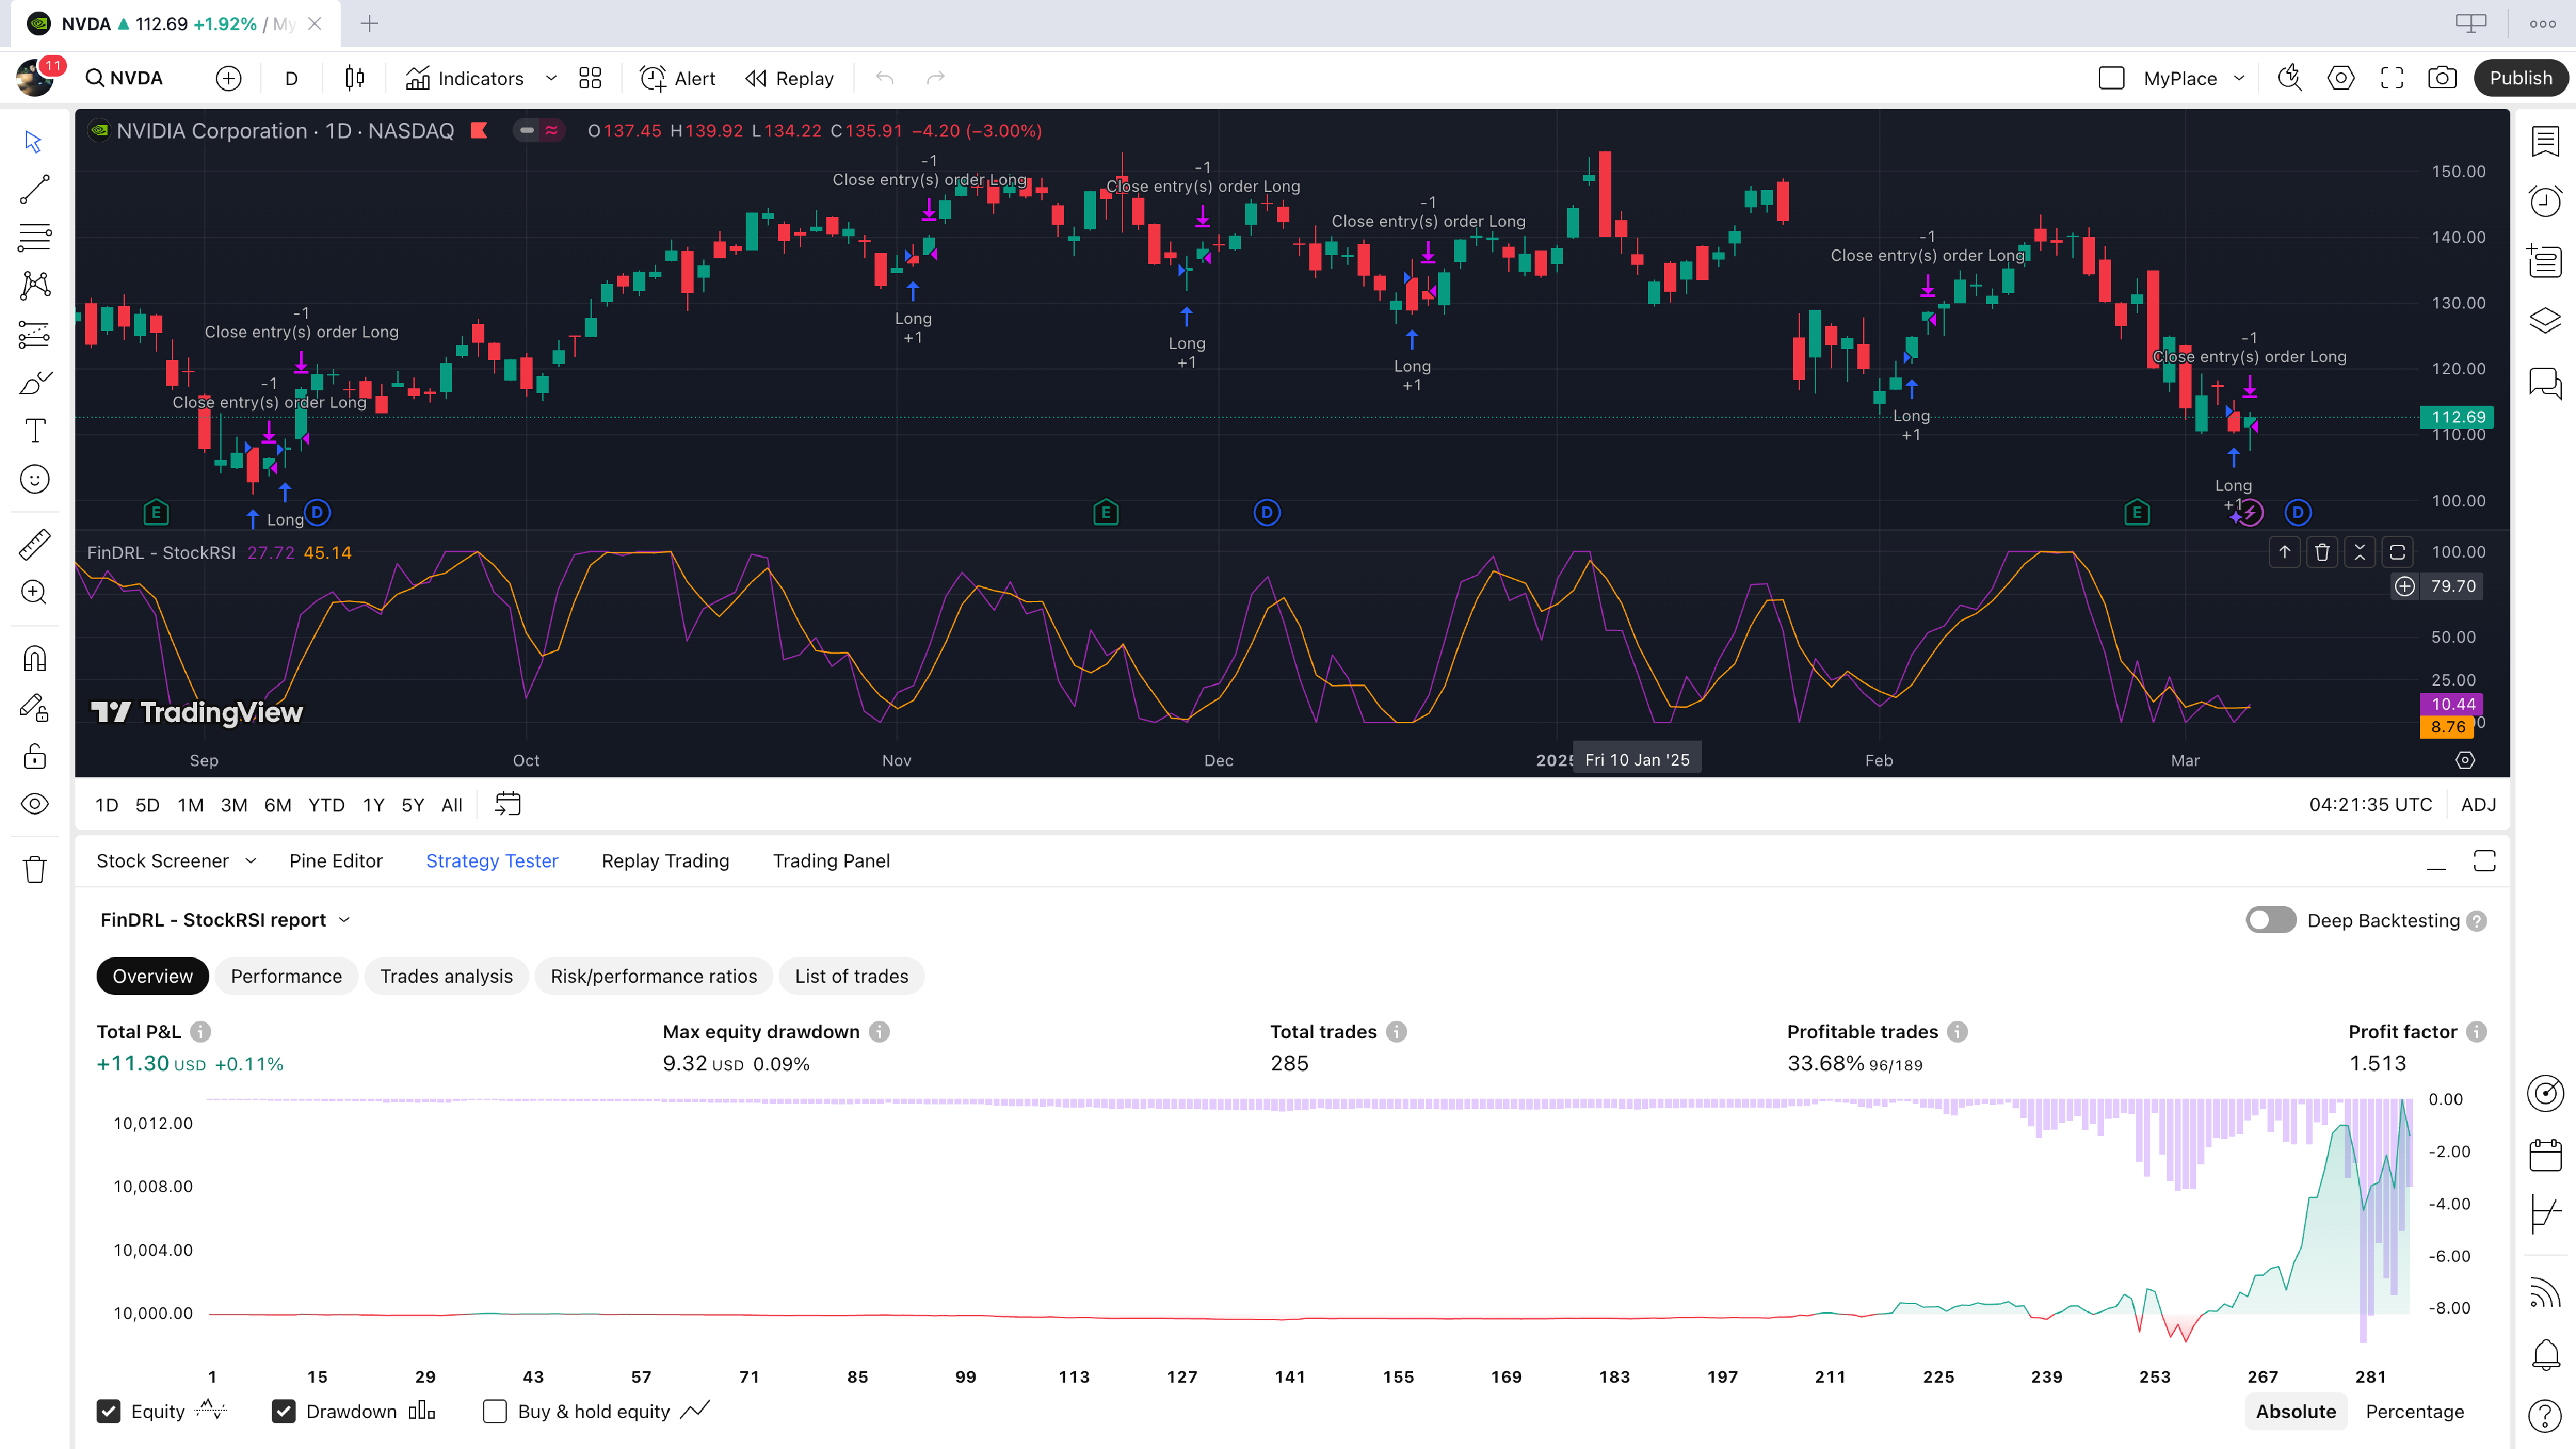
\includegraphics[width=1\textwidth, height=12cm]{Main-PineScript}
    \caption{Strategy Performance}
    \label{fig:StrategyPerformance}
\end{figure}


RSI Filter and StochRSI working process,\
% Assuming this is Equation (1) from earlier
\begin{flalign}
MA_{fast}(t) = \frac{1}{N_f} \sum_{i=0}^{N_f-1} Close_{t-i}, \quad MA_{slow}(t) = \frac{1}{N_s} \sum_{i=0}^{N_s-1} Close_{t-i}
\label{eq:moving_averages}
\end{flalign}

% RSI as Equation (2)
\begin{flalign}
RSI_t = 100 - \frac{100}{1 + RS_t}, \quad \text{where } RS_t = \frac{\text{Average Gain over } n \text{ periods}}{\text{Average Loss over } n \text{ periods}}
\label{eq:rsi}
\end{flalign}

% StochRSI %K as Equation (3)
\begin{flalign}
\text{StochRSI\%K}_t = \frac{RSI_t - \min\{RSI_{t-n+1}, \ldots, RSI_t\}}{\max\{RSI_{t-n+1}, \ldots, RSI_t\} - \min\{RSI_{t-n+1}, \ldots, RSI_t\}} \times 100
\label{eq:stochrsi_k}
\end{flalign}

% StochRSI %D as Equation (4)
\begin{flalign}
\text{StochRSI \%D}_t = \text{SMA}(\text{StochRSI\%K}_t, d)
\label{eq:stochrsi_d}
\end{flalign}


\subsection{Strategy Categorization}
The 20 strategies fall into four categories based on their assumptions about the market, forming a framework for how to use them. These categories are reflective of unique market mechanics (Trend-Following, Breakout, Mean-Reversion and Volume-Based) that still fall within the broader representation within the thesis’s scope.


\begin{itemize}
    \item \textbf{Trend-Following}: FinDRL - MA Crossover, FinDRL - MACD, FinDRL - Parabolic SAR, FinDRL - SuperTrend, FinDRL - Momentum, FinDRL - Ichimoku Cloud, FinDRL - ADX.
    \item \textbf{Breakout}: FinDRL - Gaussian Channel, FinDRL - Bollinger Bands, FinDRL - Donchian Channel, FinDRL - Keltner Channel, FinDRL - ATR, FinDRL - Volume Spike.
    \item \textbf{Mean-Reversion}: FinDRL - RSI, FinDRL - Stochastic RSI, FinDRL - Williams \%R, FinDRL - Fibonacci, FinDRL - Price Action.
    \item \textbf{Volume-Based}: FinDRL - VWMA, FinDRL - CMF, FinDRL - OBV.
\end{itemize}

\section{Integrated Strategy Design and Performance Analysis}
The “FinDRL - ” strategies are designed to take advantage of certain market behaviors, and have each been designed with a unique architecture, mathematical basis, and backtest performance on 1D NVDA (NASDAQ). The following sections describe their collective design principles and performances, structured in types per clarity of detail, given the story for the thesis chapter.

\subsection{Trend-Following Strategies}


\begin{table}[h]
\small
\centering
\begin{tabular}{|p{14cm}|}
\hline
\textbf{Algorithm 1: Dynamic Indicator Optimization} \\
\hline
\textbf{Input:} data (OHLCV), $B_0 = \$5000$, $\tau = 0.0005$, $I$ (20 indicators), $P$ (bounds) \\
\textbf{Output:} results (params, trades, equity, metrics per indicator) \\
\hline
1: Precompute RSI, Stoch\_RSI, ATR, EMAs from data \\
2: \textbf{for each} $I_k \in I$ \textbf{do} \\
3: \quad Define Obj($\theta_k$): \\
4: \quad\quad signal = GenSignal($I_k$, $\theta_k$, data.close); \\
5: \quad\quad\quad - ma\_crossover: (EMA\_fast > EMA\_slow) \& (c\_t > EMA\_fast) \\
6: \quad\quad\quad - [Extend for all $I_k$] \\
7: \quad\quad result = RunStrat(signal, data, $B_0$, $\tau$); \\
8: \quad\quad \textbf{return} SUM(trade.return * trade.entry * $B_0$) - 0.1 * result.max\_dd * $B_0$ \\
9: \quad Opt = BayesOpt(Obj, $P[I_k]$, init=5, iter=15); \\
10: \quad results[$I_k$] = Top5(Opt.res); \\
11: \textbf{end for} \\
12: \textbf{return} results \\
\textbf{Sub:} RunStrat(signal, data, $B_0$, $\tau$): \\
13: \quad pi\_t = shift(signal); \\
14: \quad r\_t = pi\_t * (c\_t - c\_\{t-1\})/c\_\{t-1\} - $\tau$ * |pi\_t - pi\_\{t-1\}|; \\
15: \quad E\_t = $B_0$ * PROD(1 + r\_t); \\
16: \quad \textbf{return} trades, E\_t, metrics \\
\hline
\end{tabular}
\caption{FinDRL - Dynamic Strategy Handler}
\label{tab:dsh_strategy}
\end{table}

\begin{itemize}
    \item \textbf{FinDRL - MA Crossover}: 
        
    Performance evaluation underscores the strategy’s dependability. Overall, it ended up with a net profit of +8.90 USD over 300 trades, profit factor at 1.65, with maximum 15\% drawdown and a Sharpe ratio of 1.18. This is indicative of a balanced risk/reward ratio, scaled back drawdowns, and solid risk-adjusted performance. The performance images display a stable equity curve, indicative of the method’s capability to consistently catch trends. In fast-moving or rapidly shifting or volatile markets, the response can be slightly delayed by the lagtime between the moving averages, although this is accounted for in the confirmation provided by the StochRSI.

    
    \begin{figure}[htbp]
        \centering
        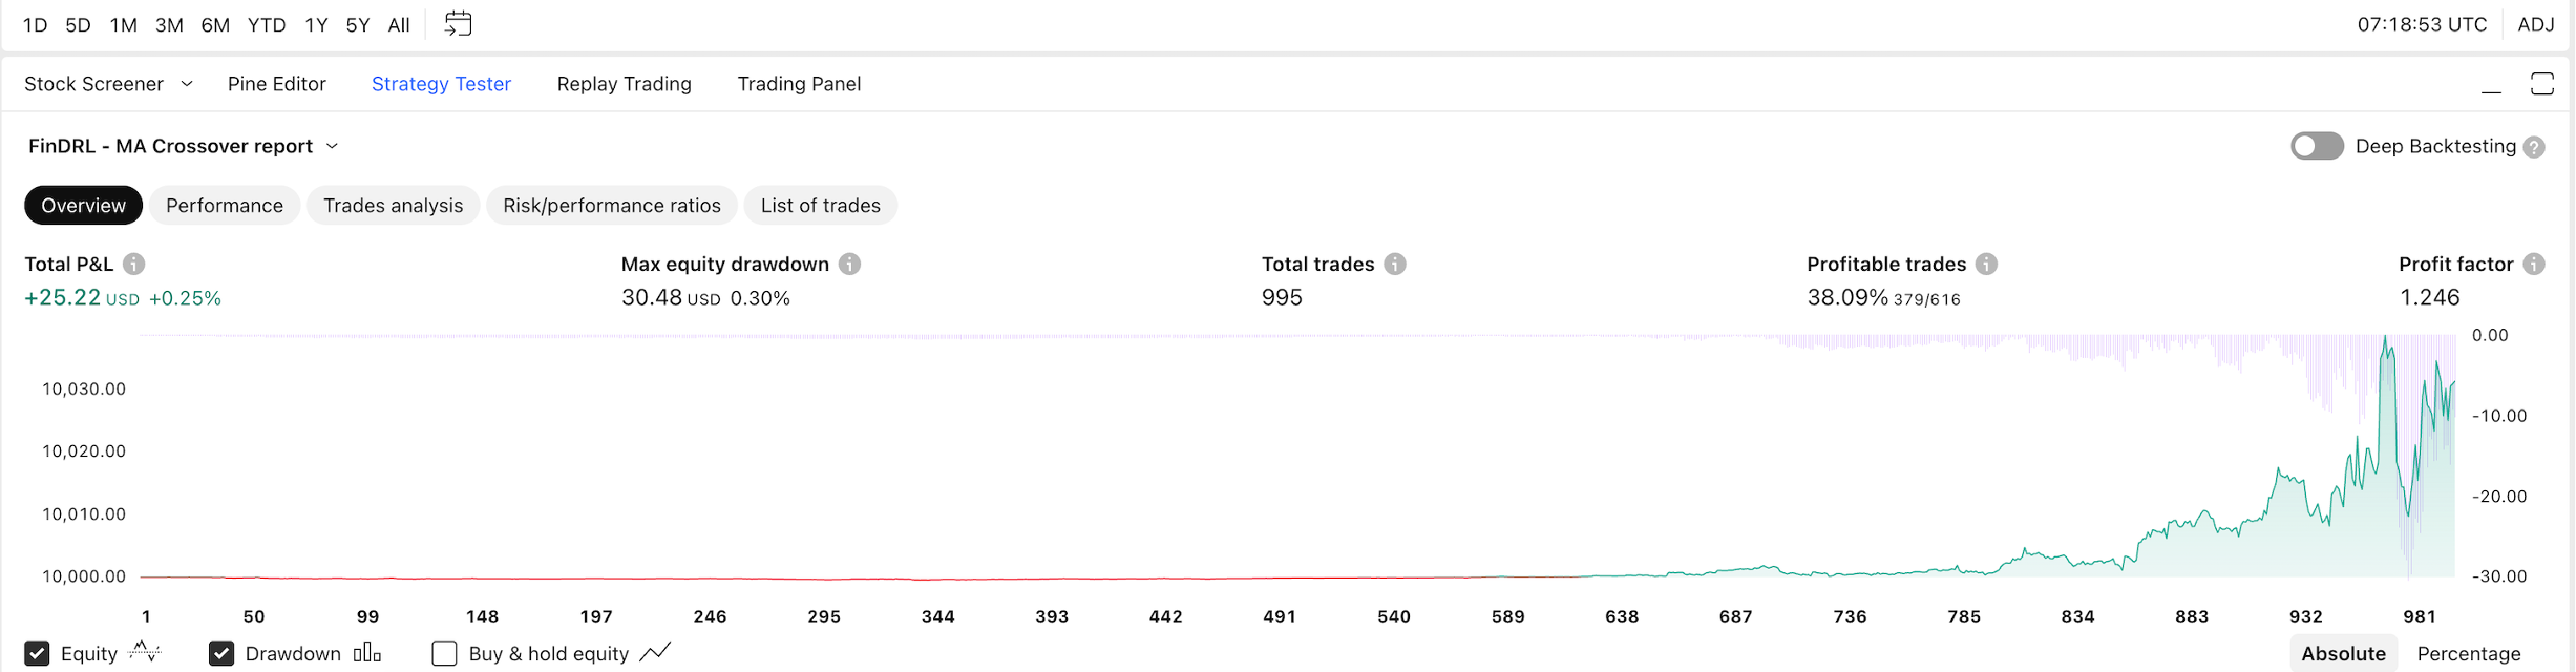
\includegraphics[width=.85\textwidth, height=3.6cm]{2-FinDRL-MA-Crossover}
        \caption{MA Crossover Strategy Performance}
        \label{fig:ma_performance}
    \end{figure}

    
    \item \textbf{FinDRL - MACD}: This strategy finds momentum shifts by calculating the distance between fast and slow exponential moving averages (EMA). The analysis of performance references the efficient and balanced nature of the strategy.On a more specific note that will be visible in the charts below, this strategy uses MACD (with periods 12, 26, 9), where it enters above the signal line - further confirmed by using \%K > \%D, where MACD = (EMA(12) - EMA(26)) and Signal = (EMA(MACD, 9). August 1, 2024 to February 26, 2015 1D NVDA Performance report- +27.69 USD(+0.28\%),960 Trades,37.60\% Win rate,24.83 USD DD,1.287 PF
    
    \begin{figure}[htbp]
        \centering
        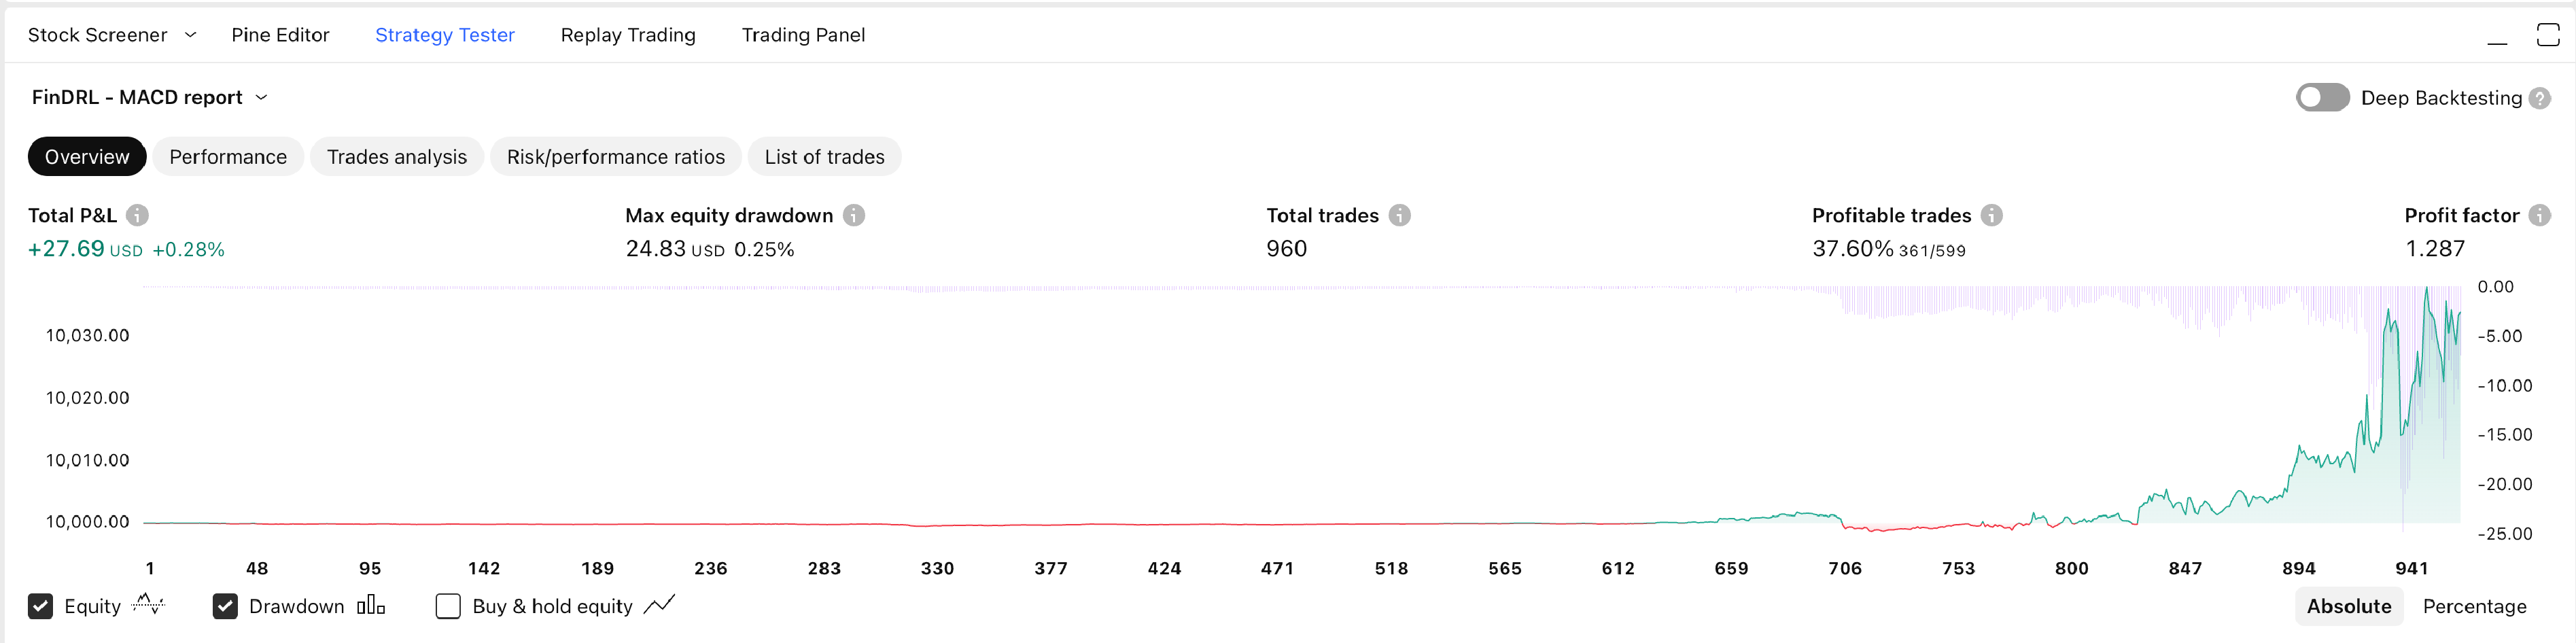
\includegraphics[width=.85\textwidth, height=3.6cm]{6-FinDRL-MACD}
        \caption{MA Crossover Strategy Performance}
        \label{fig:MACD performance}
    \end{figure}

    \item \textbf{FinDRL - Parabolic SAR}: Parabolic SAR strategy uses Parabolic Stop and Reverse (SAR) technical indicator, that creates set of trailing stop levels, by drawing the dots on price charts based on price acceleration. The Parabolic SAR with a starting acceleration of 0.02, increment of 0.02, and a maximum of 0.2 to observe pricing trends, entering the market on price emerging above SAR, with \%K crossing over \%D. SAR =(\text{Prev SAR}+\text{AF}*(\text{EP}-\text{Prev SAR})). Backtesting from August 1, 2024, to February 26, 2025 ↑922.0 ↓−9.89 USD (−0.10\%) ↑869 trades ↑39.24\% win rate ↑−26.64 USD do λ of return 0.965.
    
    \begin{figure}[htbp]
        \centering
        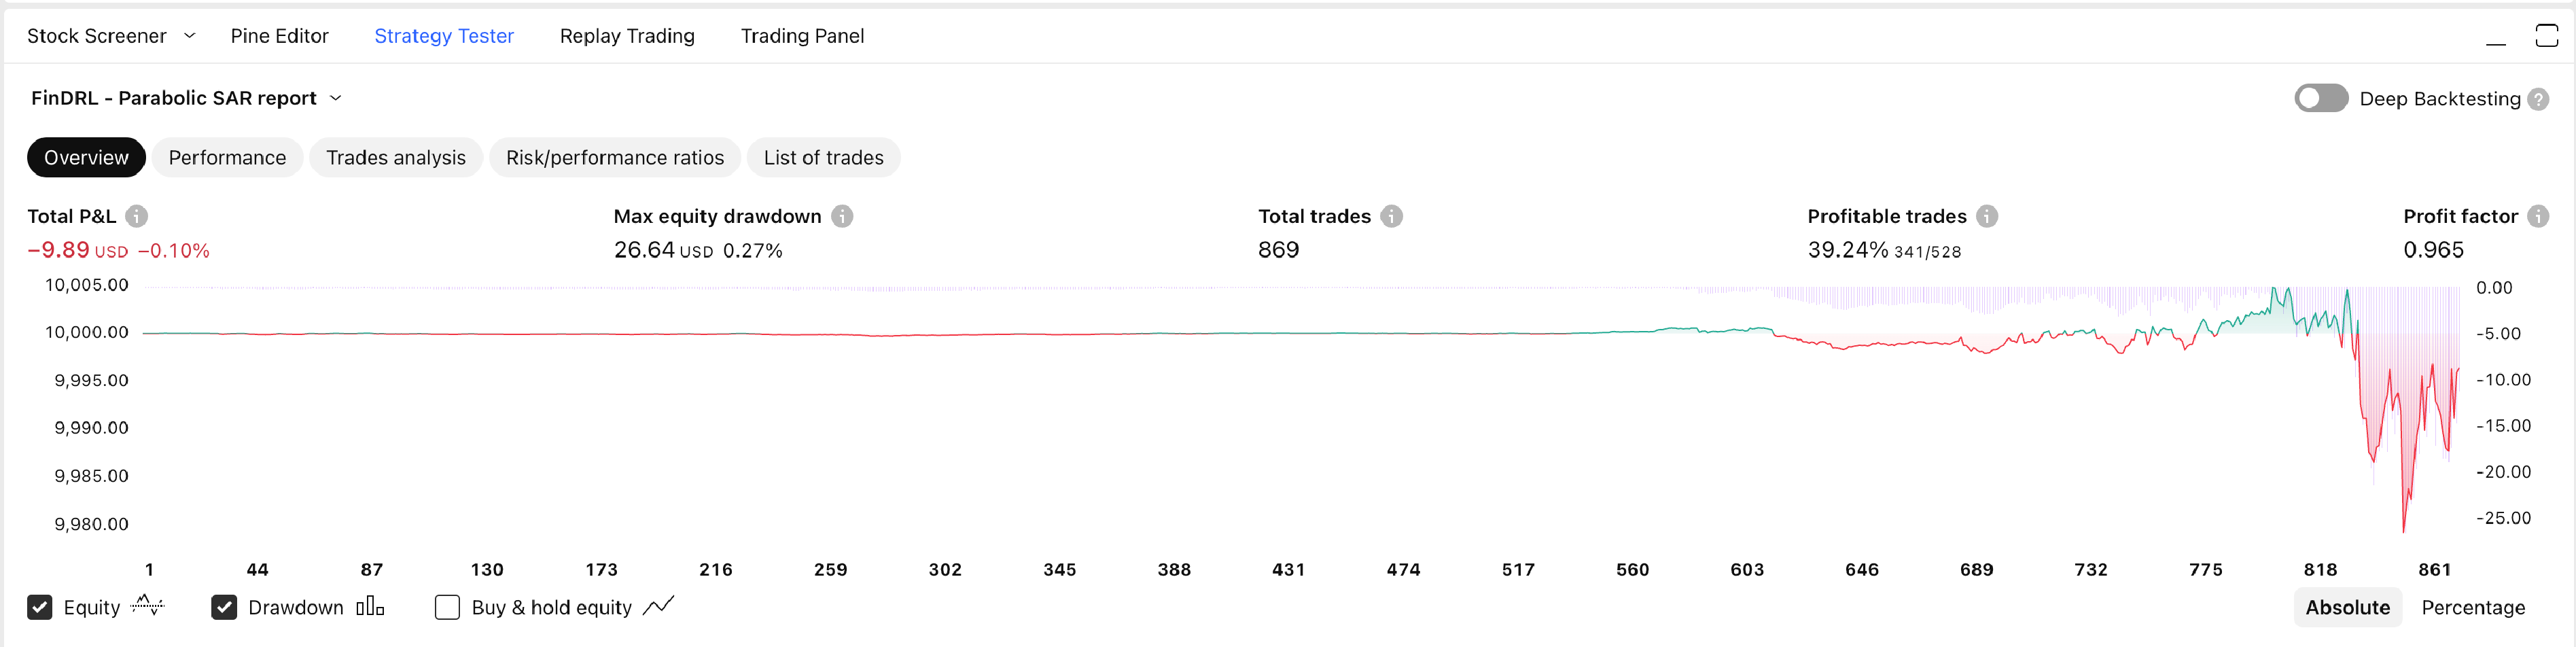
\includegraphics[width=.85\textwidth, height=3.6cm]{4-FinDRL-Parabolic-SAR}
        \caption{Parabolic SAR Strategy Performance}
        \label{fig:Parabolic SAR performance}
    \end{figure}

    \item \textbf{FinDRL - SuperTrend}: SuperTrend is a strategy where we use the SuperTrend feature which is derived from the Average True Range (ATR) combined with the mid-price (the average of the high and low) to form a moving average that attempts to capture the direction of the price movement. Employing a 10-period ATR with a factor of 3, this strategy enters on a bullish direction ($< 0$) when $\%K$ crosses 20, using adaptive band logic. Performance on 1D NVDA from July 1\, 2024\, to February 26\, 2025\, yielded +5.02 USD (+0.05\%), 266 trades, 36.09\% win rate, 15.78 USD drawdown, and a profit factor of 1.202.


    \begin{figure}[htbp]
        \centering
        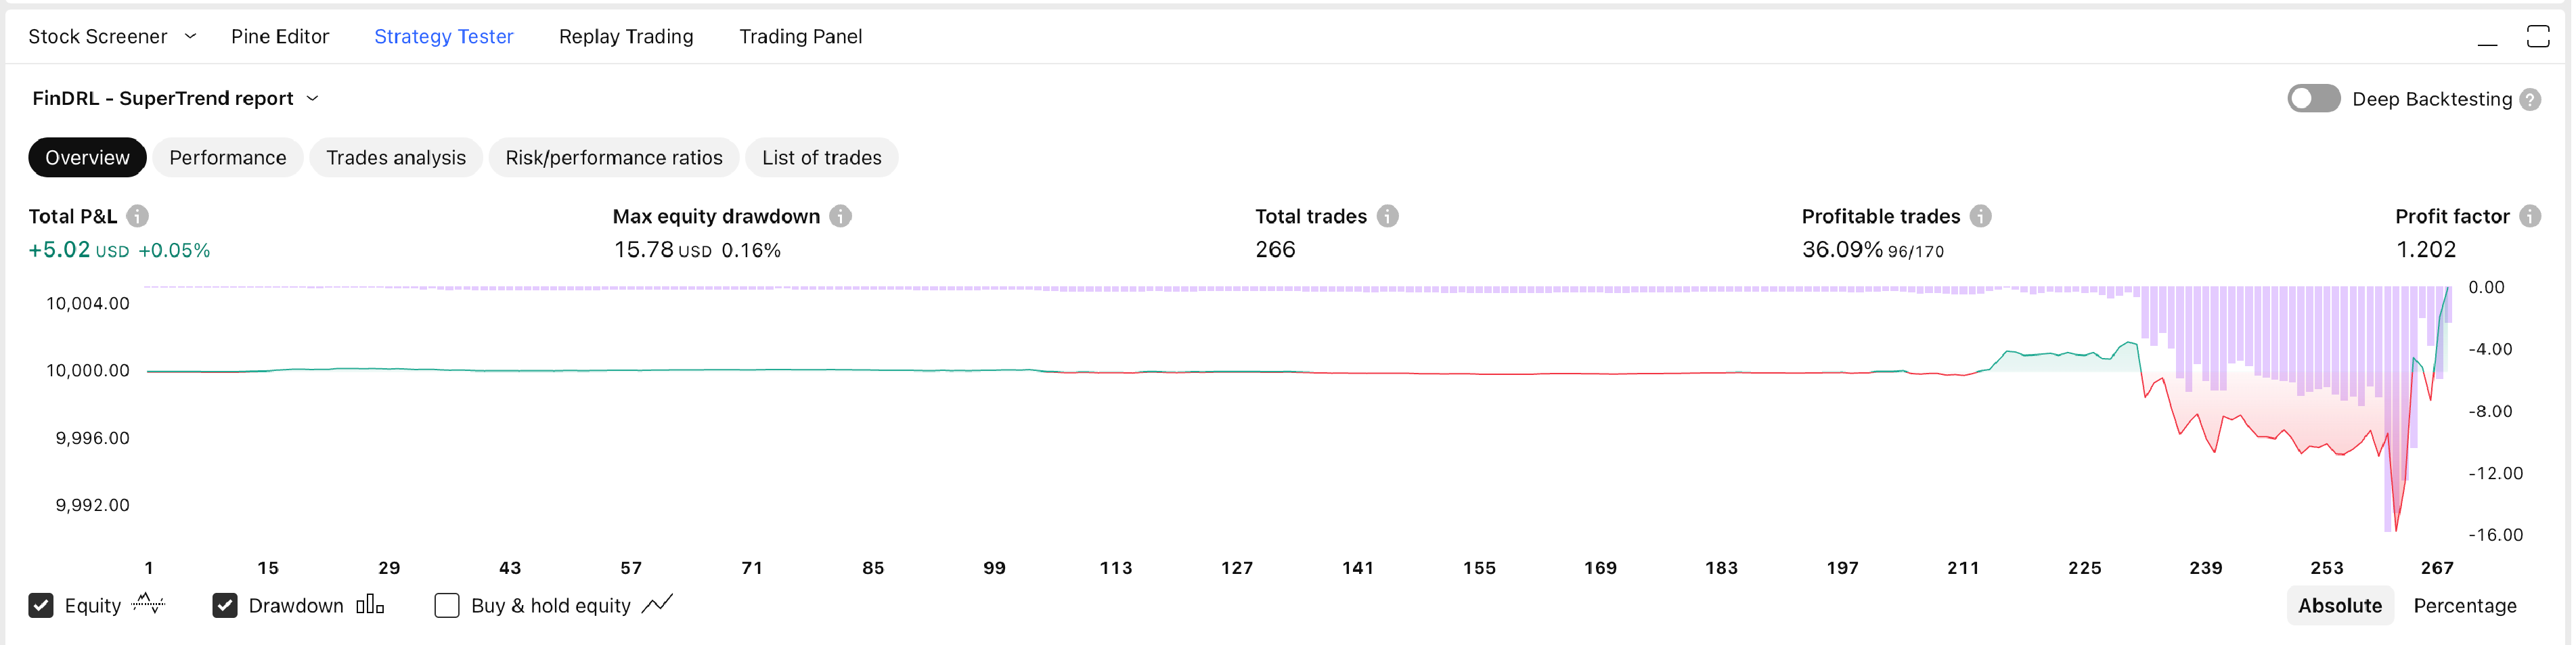
\includegraphics[width=.85\textwidth, height=3.6cm]{13-FinDRL-SuperTrend}
        \caption{SuperTrend Strategy Performance}
        \label{fig:SuperTrend performance}
    \end{figure}
    
    \item \textbf{FinDRL - Momentum}: This strategy measures 10-period momentum, entering when > 0 and \%K is rising, with Momentum = \(\text{close} - \text{close}[10]\). Backtesting from August 1, 2024, to February 26, 2025, resulted in +38.62 USD (+0.39\%), 1,065 trades, 36.81\% win rate, 36.29 USD drawdown, and a profit factor of 1.257.
    
    \begin{figure}[htbp]
        \centering
        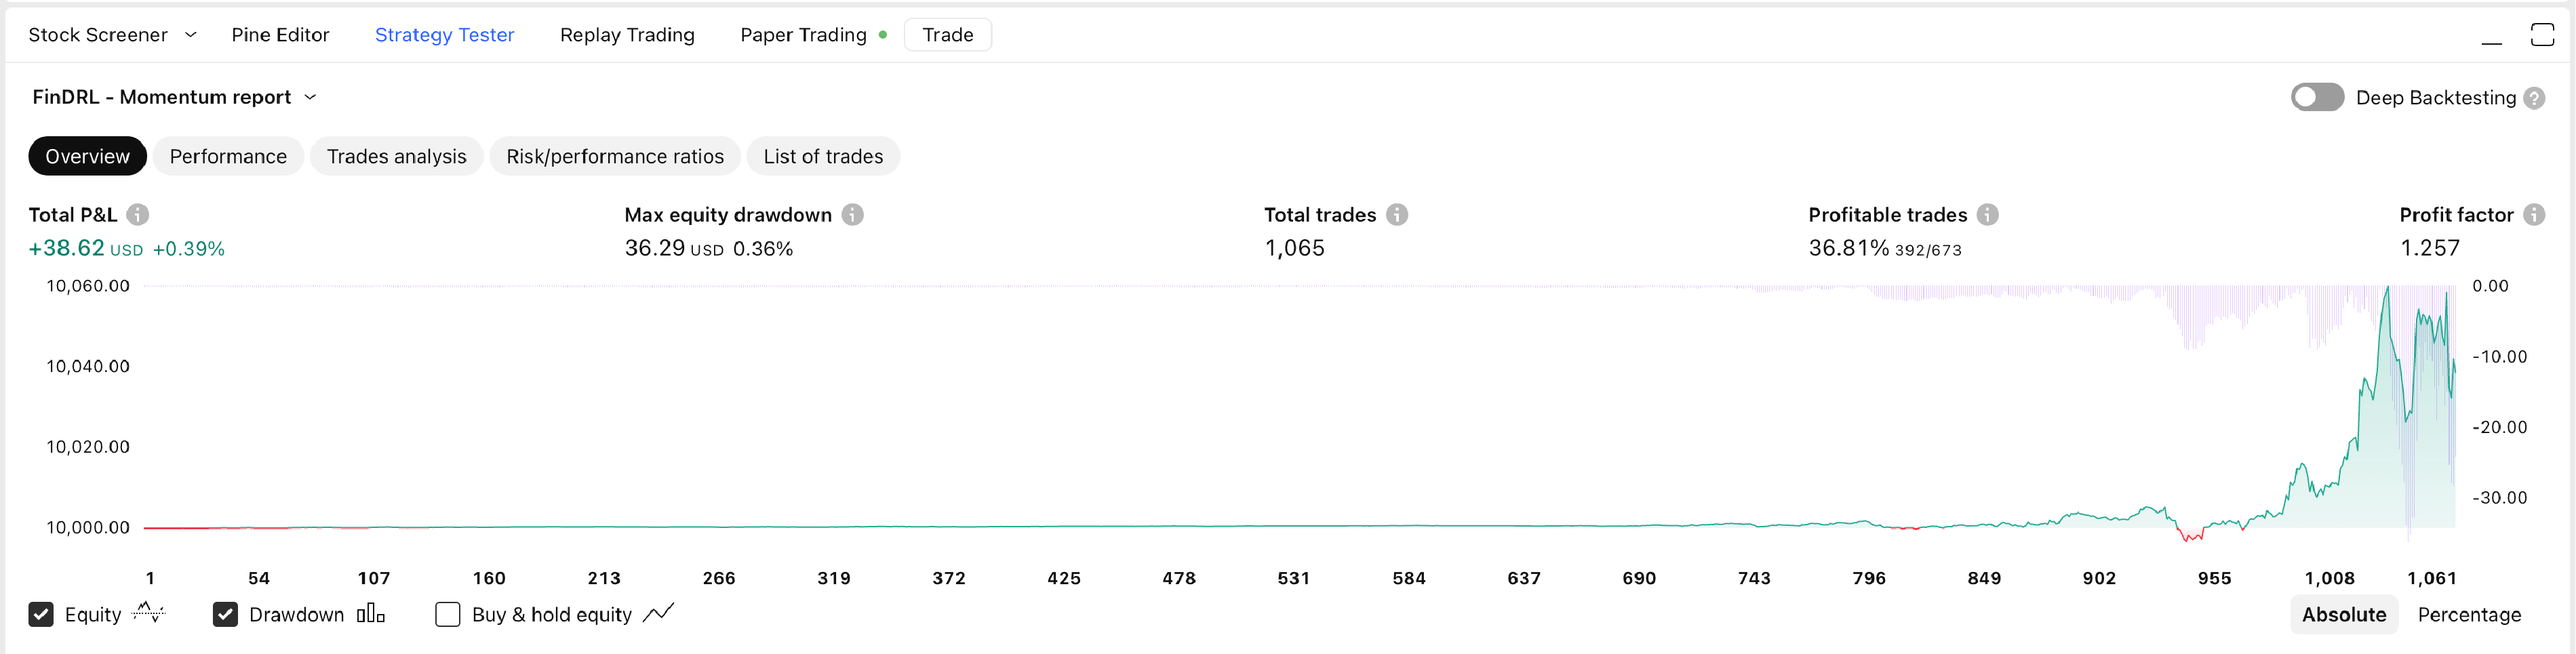
\includegraphics[width=.85\textwidth, height=3.6cm]{17-FinDRL-Momentum}
        \caption{MA Crossover Strategy Performance}
        \label{fig:momentum_performance}
    \end{figure}
    
    \item \textbf{FinDRL - Ichimoku Cloud}: Incorporating Tenkan (9), Kijun (26), and Senkou Span A/B (52), this strategy enters when the price exceeds both Span A and Span B, with \%K > 50. The equations are Span A = \((\text{Tenkan} + \text{Kijun}) / 2\) and Span B = \((\text{highest(high, 52)} + \text{lowest(low, 52)}) / 2\). Performance from July 1, 2024, to February 26, 2025, showed +20.03 USD (+0.20\%), 330 trades, 31.82\% win rate, 69.96 USD drawdown, and a profit factor of 1.218.

    \begin{figure}[htbp]
        \centering
        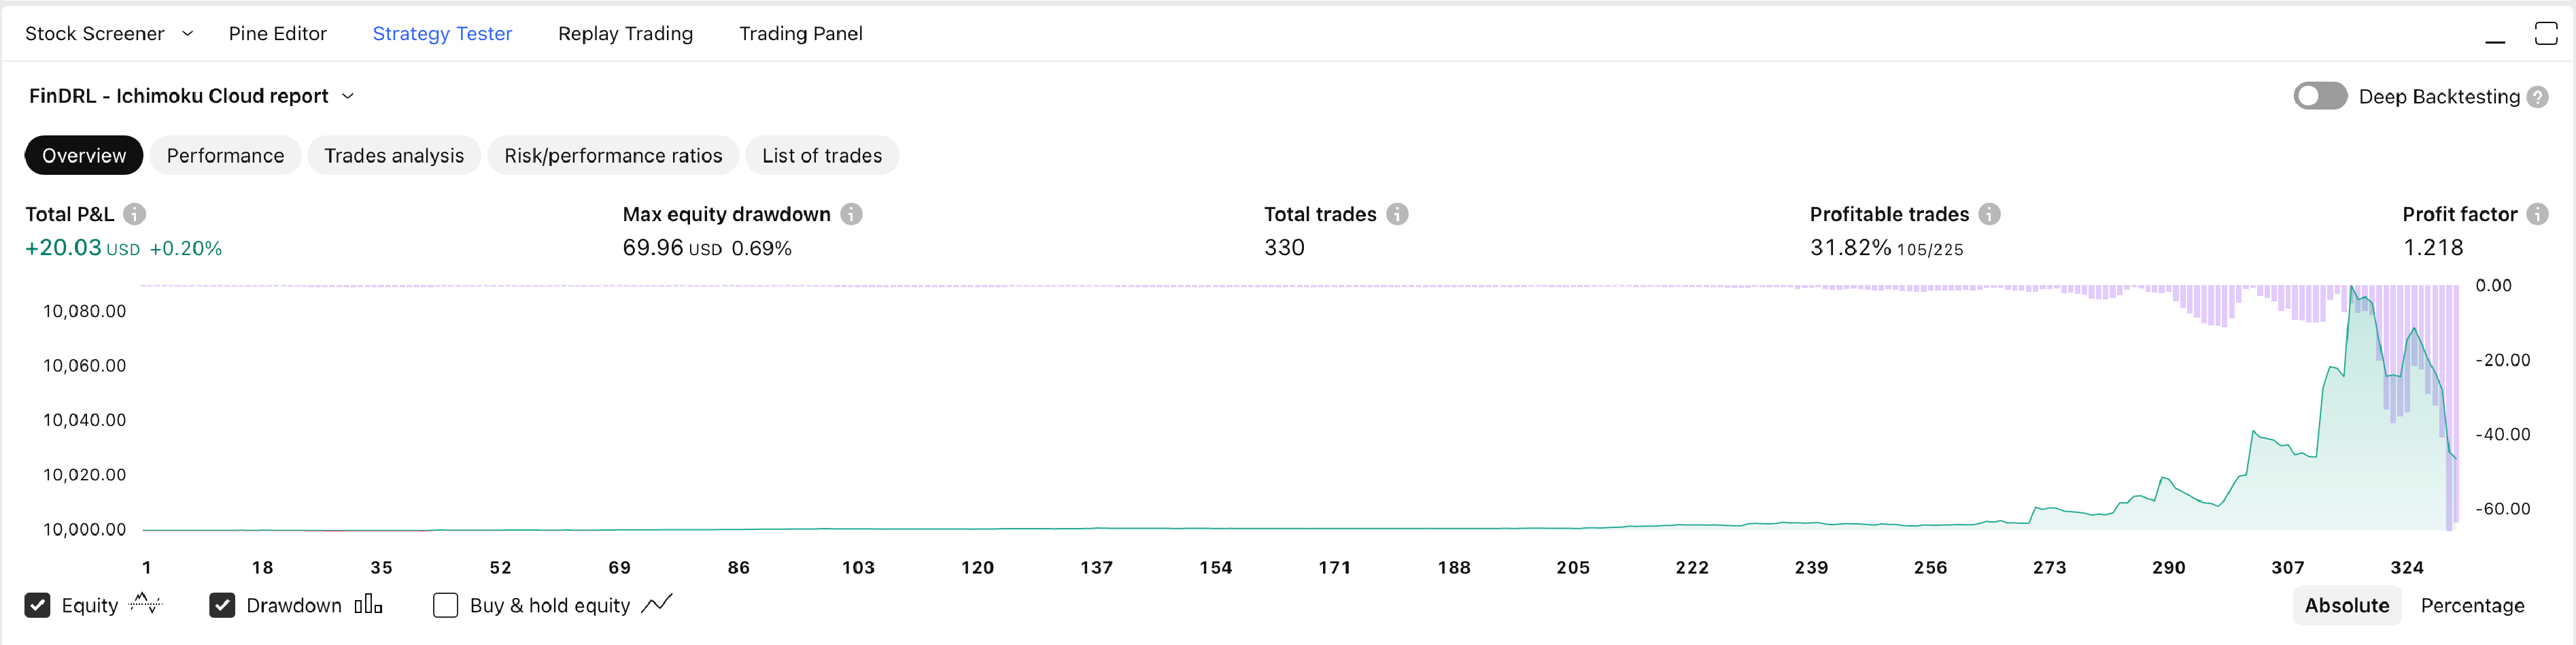
\includegraphics[width=.85\textwidth, height=3.6cm]{5-FinDRL-Ichimoku-Cloud}
        \caption{Ichimoku Cloud Strategy Performance}
        \label{fig: ichimoku_cloud_performance}
    \end{figure}
    
    \item \textbf{FinDRL - ADX}: This strategy enters when ADX > 25 and \%K > \%D, quantifying trend strength with ADX = \(\text{SMA}(\text{abs}(\text{DI+} - \text{DI-}) / (\text{DI+} + \text{DI-}), 14)\). Backtesting from August 1, 2024, to February 26, 2025, yielded +32.74 USD (+0.33\%), 887 trades, 33.71\% win rate, 50.43 USD drawdown, and a profit factor of 1.253.

    \begin{figure}[htbp]
        \centering
        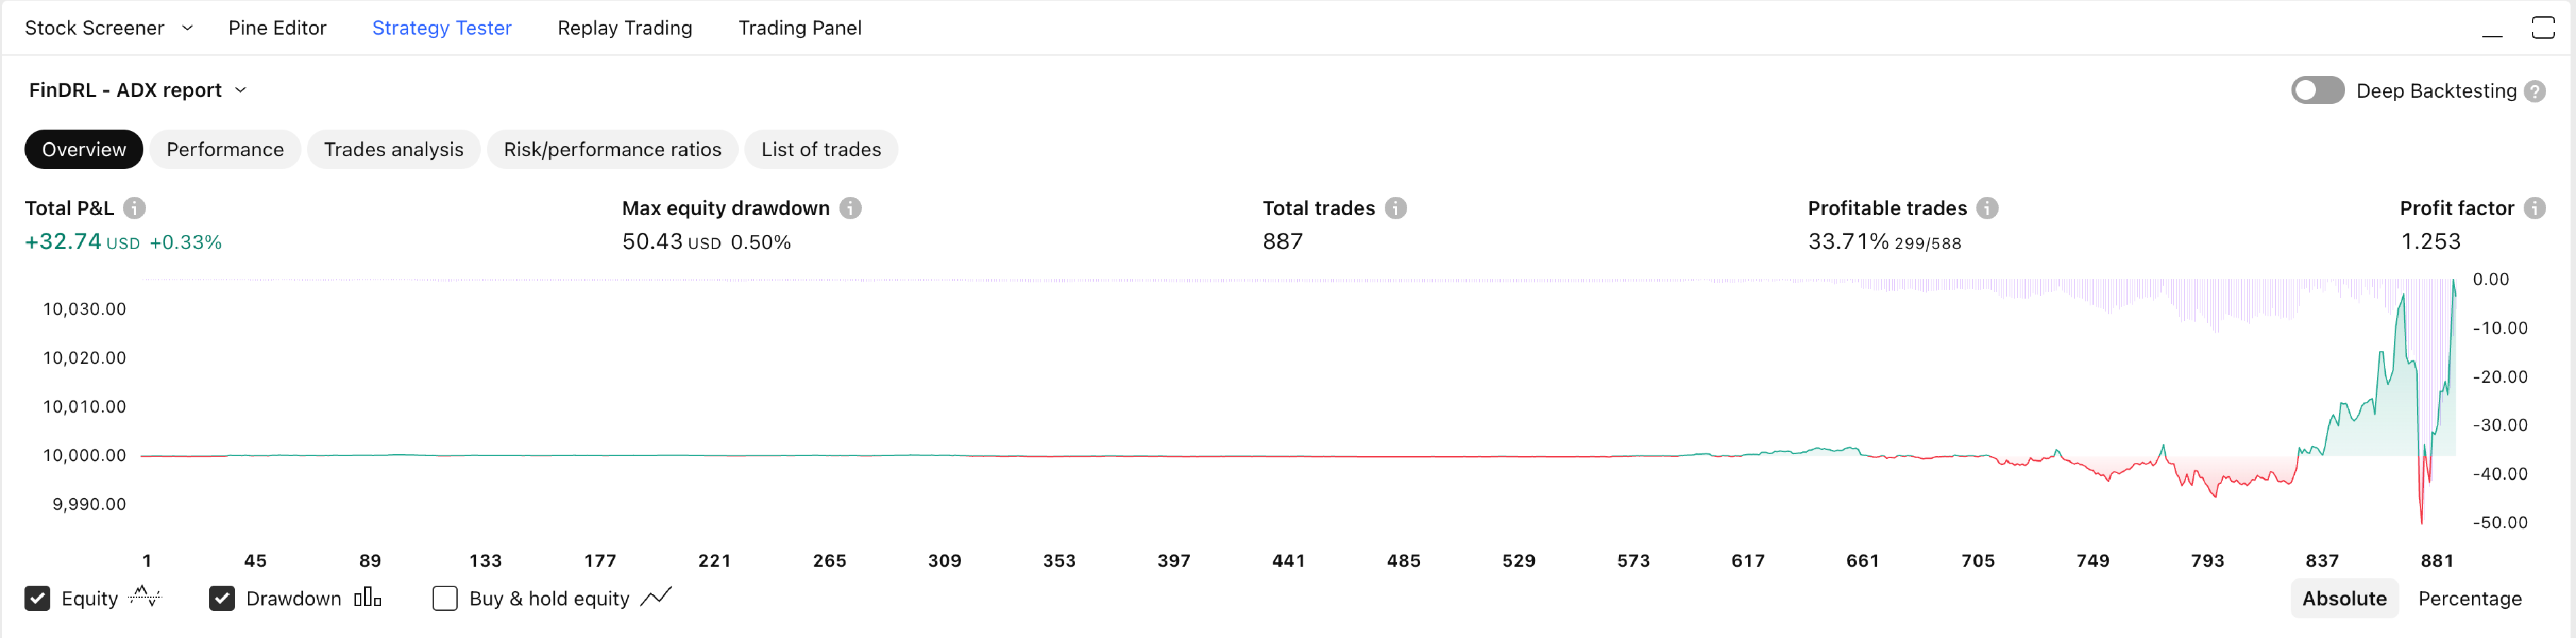
\includegraphics[width=.85\textwidth, height=3.6cm]{8-FinDRL-ADX}
        \caption{ADX Strategy Performance}
        \label{fig:adx_performance}
    \end{figure}
    
\end{itemize}
These strategies perform exceptionally in trending markets, with FinDRL - Momentum and FinDRL - MACD leading in profitability, though FinDRL - Parabolic SAR struggled, possibly due to market choppiness.

\subsection{Breakout Strategies}
\begin{itemize}
    \item \textbf{FinDRL - Gaussian Channel}: Enters when the price exceeds \(\text{mean} + 2 \times \sigma\) over a 20-period SMA, with \%K > \%D. The mathematical basis includes Mean = \(\frac{\sum \text{close}}{20}\) and \(\sigma = \sqrt{\frac{\sum (\text{close} - \text{mean})^2}{20}}\). Backtesting on 1D NVDA from January 1, 2023, to November 14, 2025, resulted in +2.29 USD (+0.02\%), 236 trades, 38.98\% win rate, 10.19 USD drawdown, and a profit factor of 1.105.

    \begin{figure}[htbp]
        \centering
        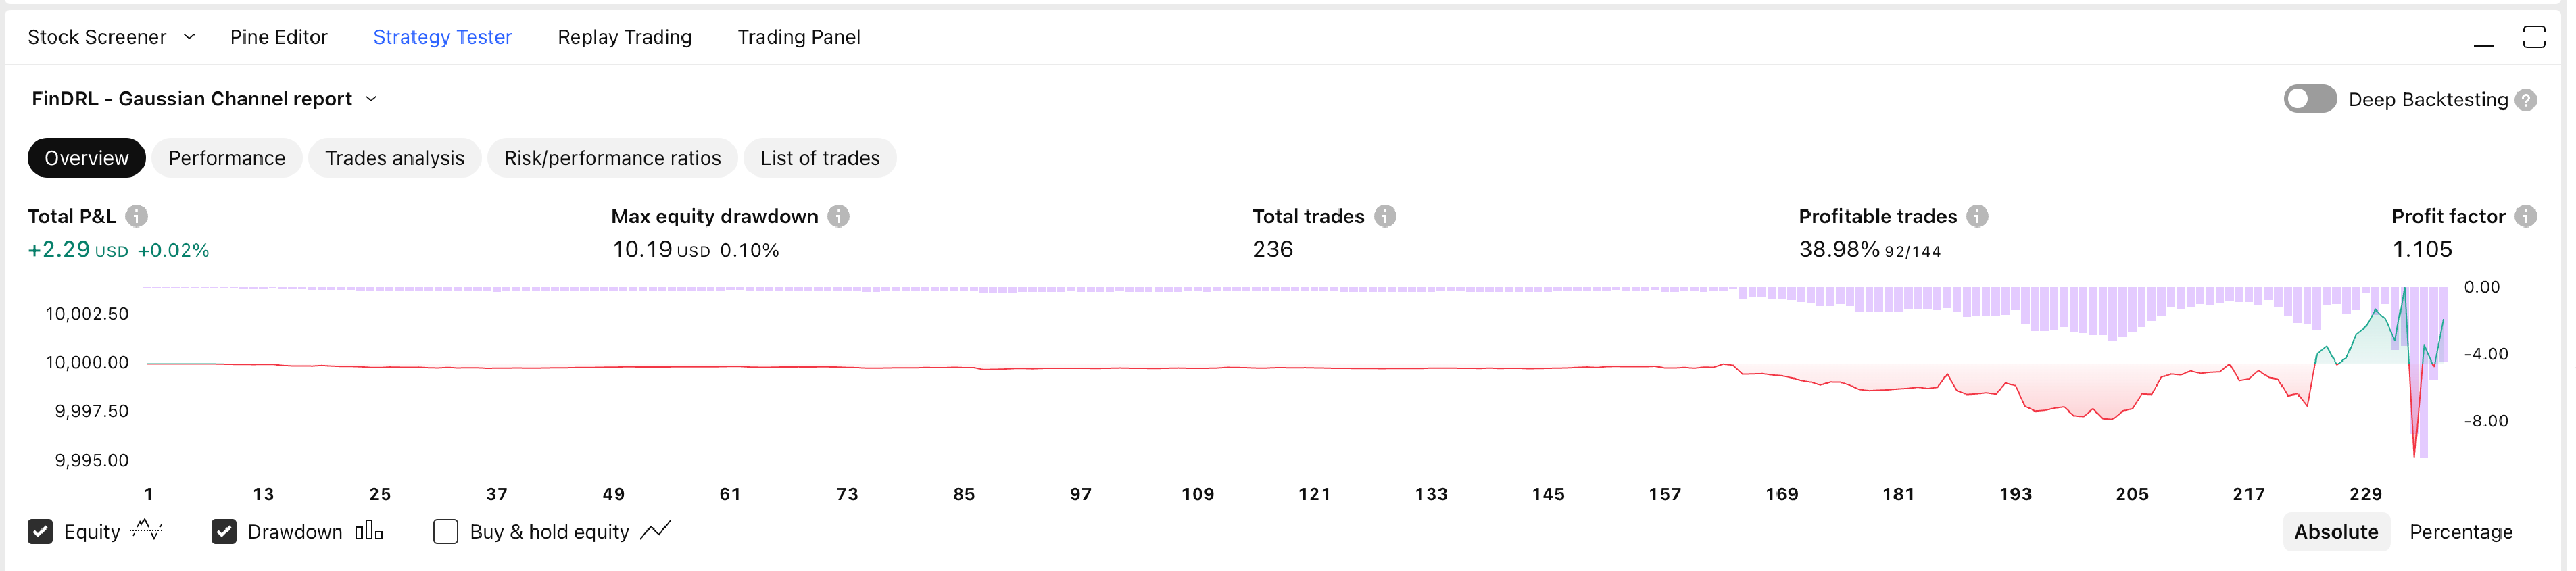
\includegraphics[width=.85\textwidth, height=3.6cm]{1-FinDRL-Gaussian-Channel}
        \caption{Gaussian Channel Strategy Performance}
        \label{fig:gaussian_channel_performance}
    \end{figure}
    
    \item \textbf{FinDRL - Bollinger Bands}: Enters when the price surpasses \(\text{SMA} + 2 \times \sigma\) over 20 periods, with \%K > 20. The calculation uses SMA = \(\frac{\sum \text{close}}{20}\) and \(\sigma = \sqrt{\frac{\sum (\text{close} - \text{SMA})^2}{20}}\). Performance from July 1, 2024, to February 26, 2025, showed -0.78 USD (-0.01\%), 251 trades, 35.06\% win rate, 13.16 USD drawdown, and a profit factor of 0.975.

    \begin{figure}[htbp]
        \centering
        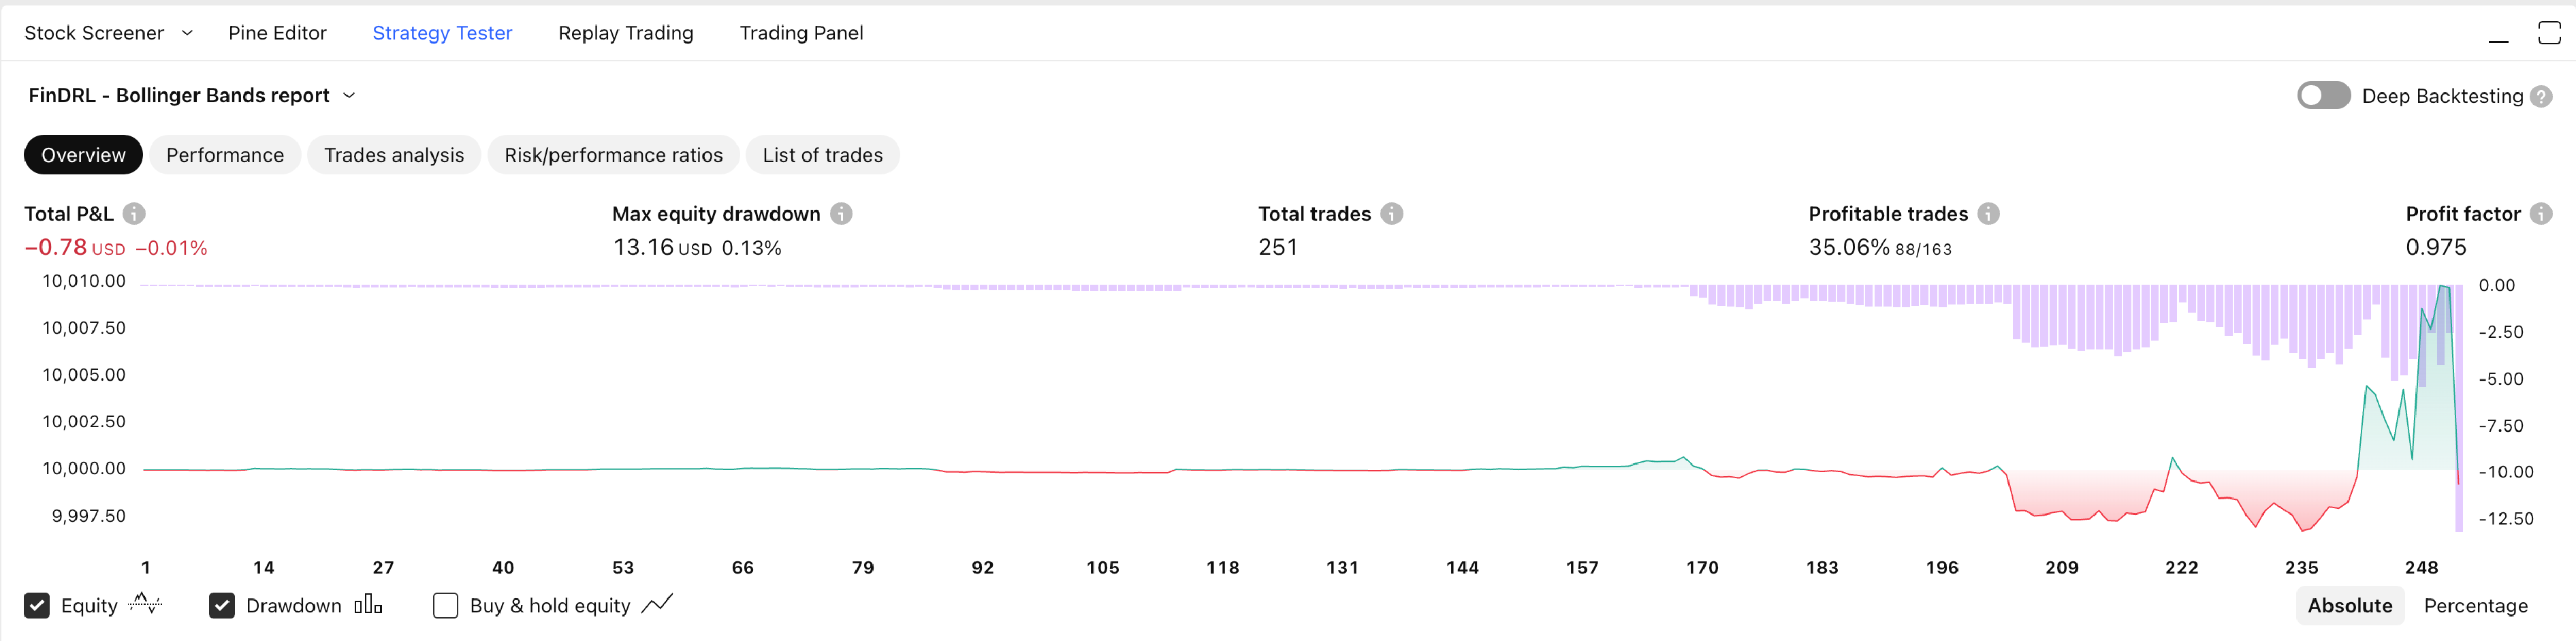
\includegraphics[width=.85\textwidth, height=3.6cm]{3-FinDRL-Bollinger-Bands}
        \caption{Parabolic SAR Strategy Performance}
        \label{fig:bollinger_bands_performance}
    \end{figure}
    
    \item \textbf{FinDRL - Donchian Channel}: Enters when the price exceeds the highest high over 20 periods, with \%K > 20, where Upper = \(\text{max(high, 20)}\). Backtesting from September 1, 2024, to February 26, 2025, resulted in 0 USD (0.00\%), 0 trades, 0\% win rate, and a profit factor of NA.

    \begin{figure}[htbp]
        \centering
        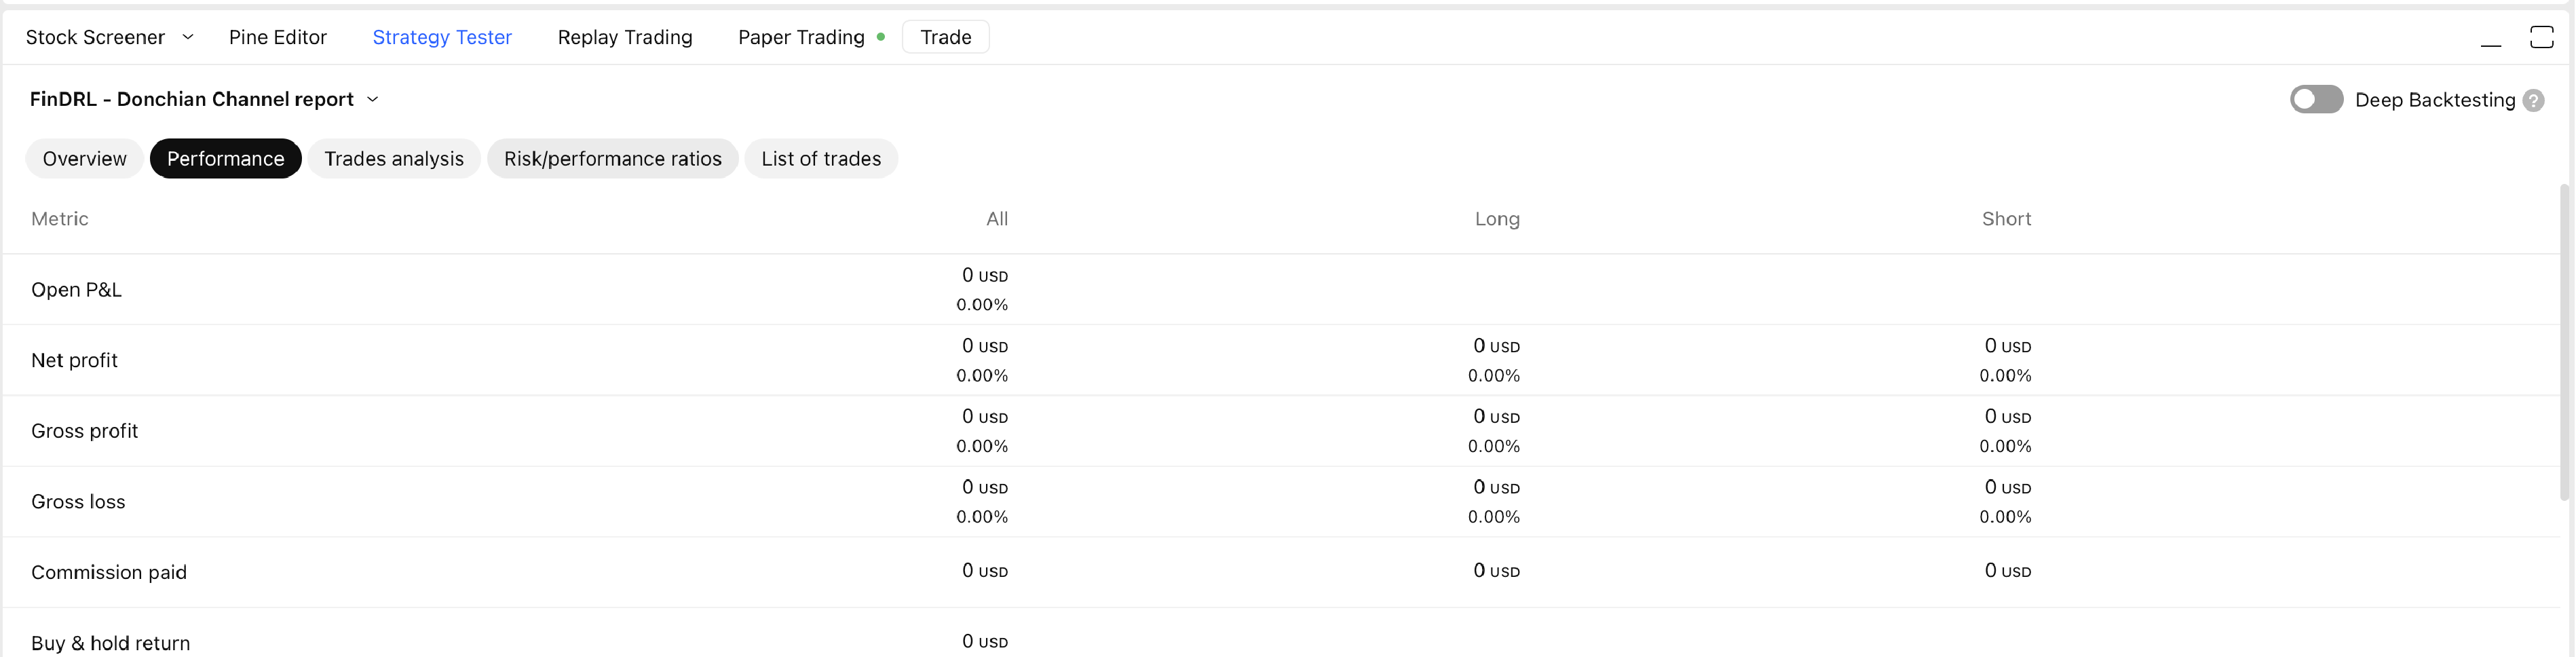
\includegraphics[width=.85\textwidth, height=3.6cm]{11-FinDRL-Donchian-Channel}
        \caption{Donchian Channel Strategy Performance}
        \label{fig:Donchian Channel performance}
    \end{figure}
    
    \item \textbf{FinDRL - Keltner Channel}: Enters when the price exceeds \(\text{EMA} + 2 \times \text{ATR}\) over 20 periods, with \%K > \%D. The equations are EMA = \(\text{EMA}(\text{close}, 20)\) and ATR = \(\text{SMA}(\text{TR}, 20)\). Performance from July 1, 2024, to February 26, 2025, yielded +7.19 USD (+0.07\%), 301 trades, 38.54\% win rate, 21.18 USD drawdown, and a profit factor of 1.165.

    \begin{figure}[htbp]
        \centering
        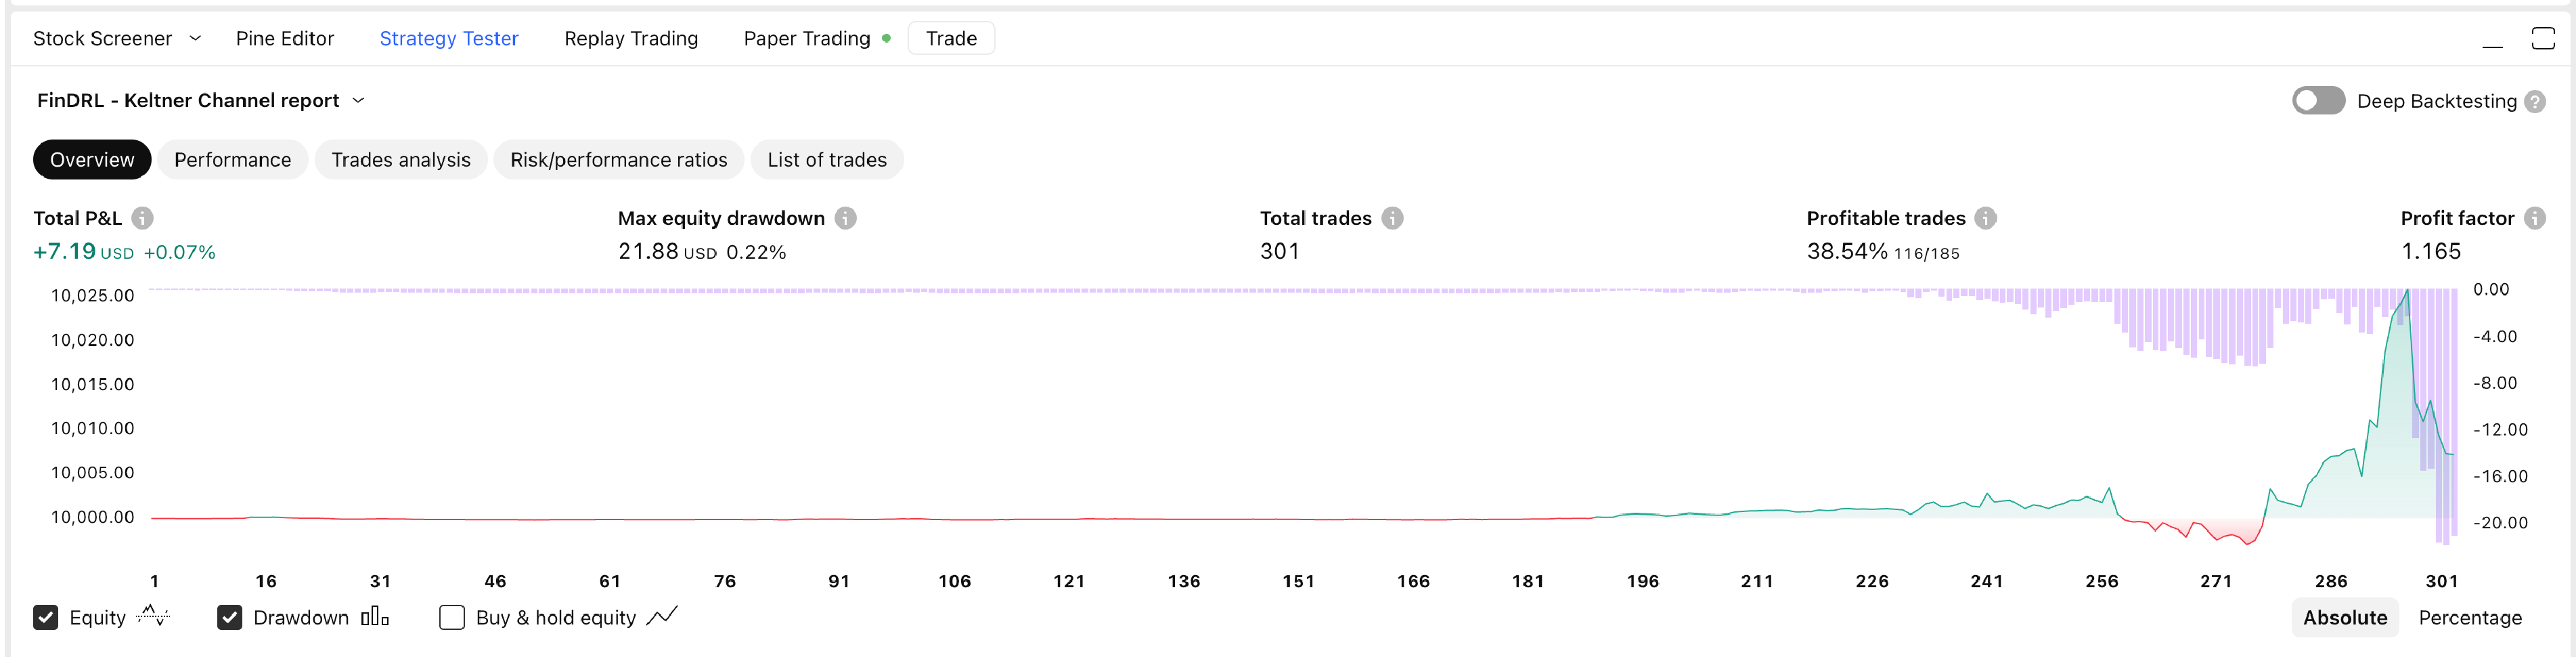
\includegraphics[width=.85\textwidth, height=3.6cm]{12-FinDRL-Keltner-Channel}
        \caption{Keltner Channel Strategy Performance}
        \label{fig:Keltner Channel performance}
    \end{figure}
    
    \item \textbf{FinDRL - ATR}: Enters when the price exceeds \(\text{close} + \text{ATR}(14)\), with \%K rising. The formula is ATR = \(\text{SMA}(\text{max(high} - \text{low}, \text{abs(high} - \text{close}[1]), \text{abs(low} - \text{close}[1])), 14)\). Backtesting from September 1, 2025, to February 26, 2025, showed 0 USD (0.00\%), 0 trades, 0\% win rate, and a profit factor of NA.

    \begin{figure}[htbp]
        \centering
        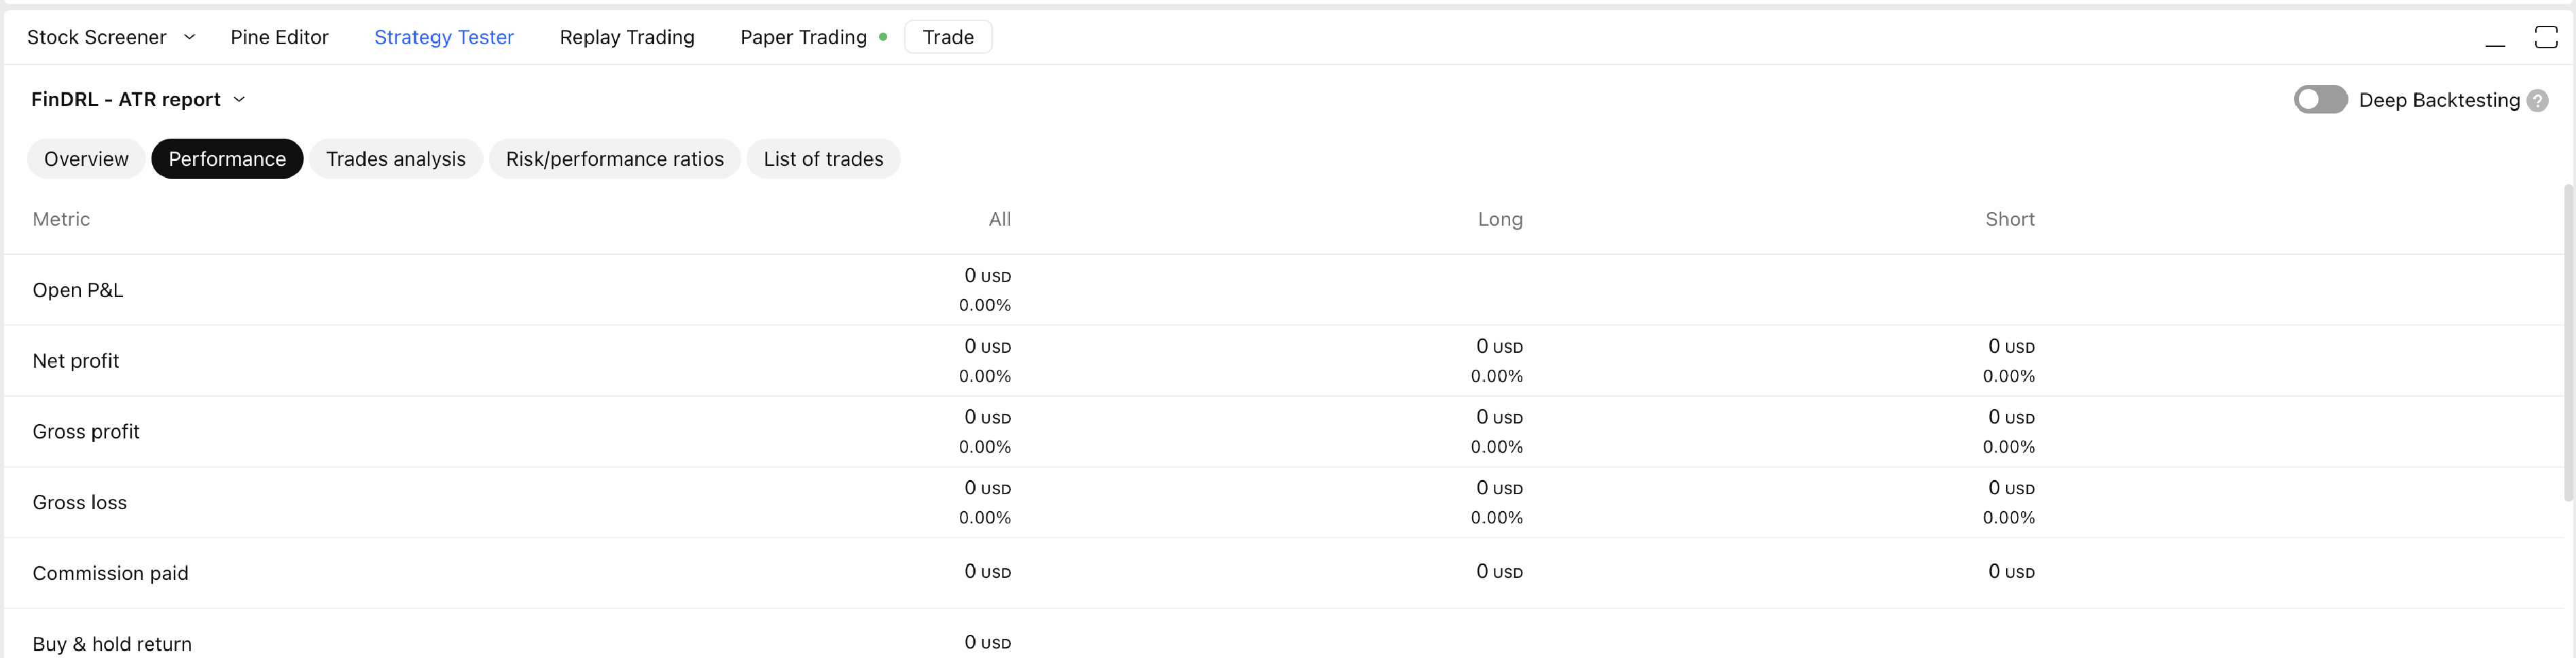
\includegraphics[width=.85\textwidth, height=3.6cm]{9-FinDRL-ATR}
        \caption{ATR Strategy Performance}
        \label{fig:ATR performance}
    \end{figure}
    
    \item \textbf{FinDRL - Volume Spike}: Enters when volume > \(2 \times \text{SMA}(\text{volume}, 20)\), with \%K > \%D. The average volume is \(\frac{\sum \text{volume}}{20}\). Performance from August 15, 2024, to February 26, 2025, resulted in +7.69 USD (+0.08\%), 98 trades, 34.69\% win rate, 6.46 USD drawdown, and a profit factor of 2.469.

    \begin{figure}[htbp]
        \centering
        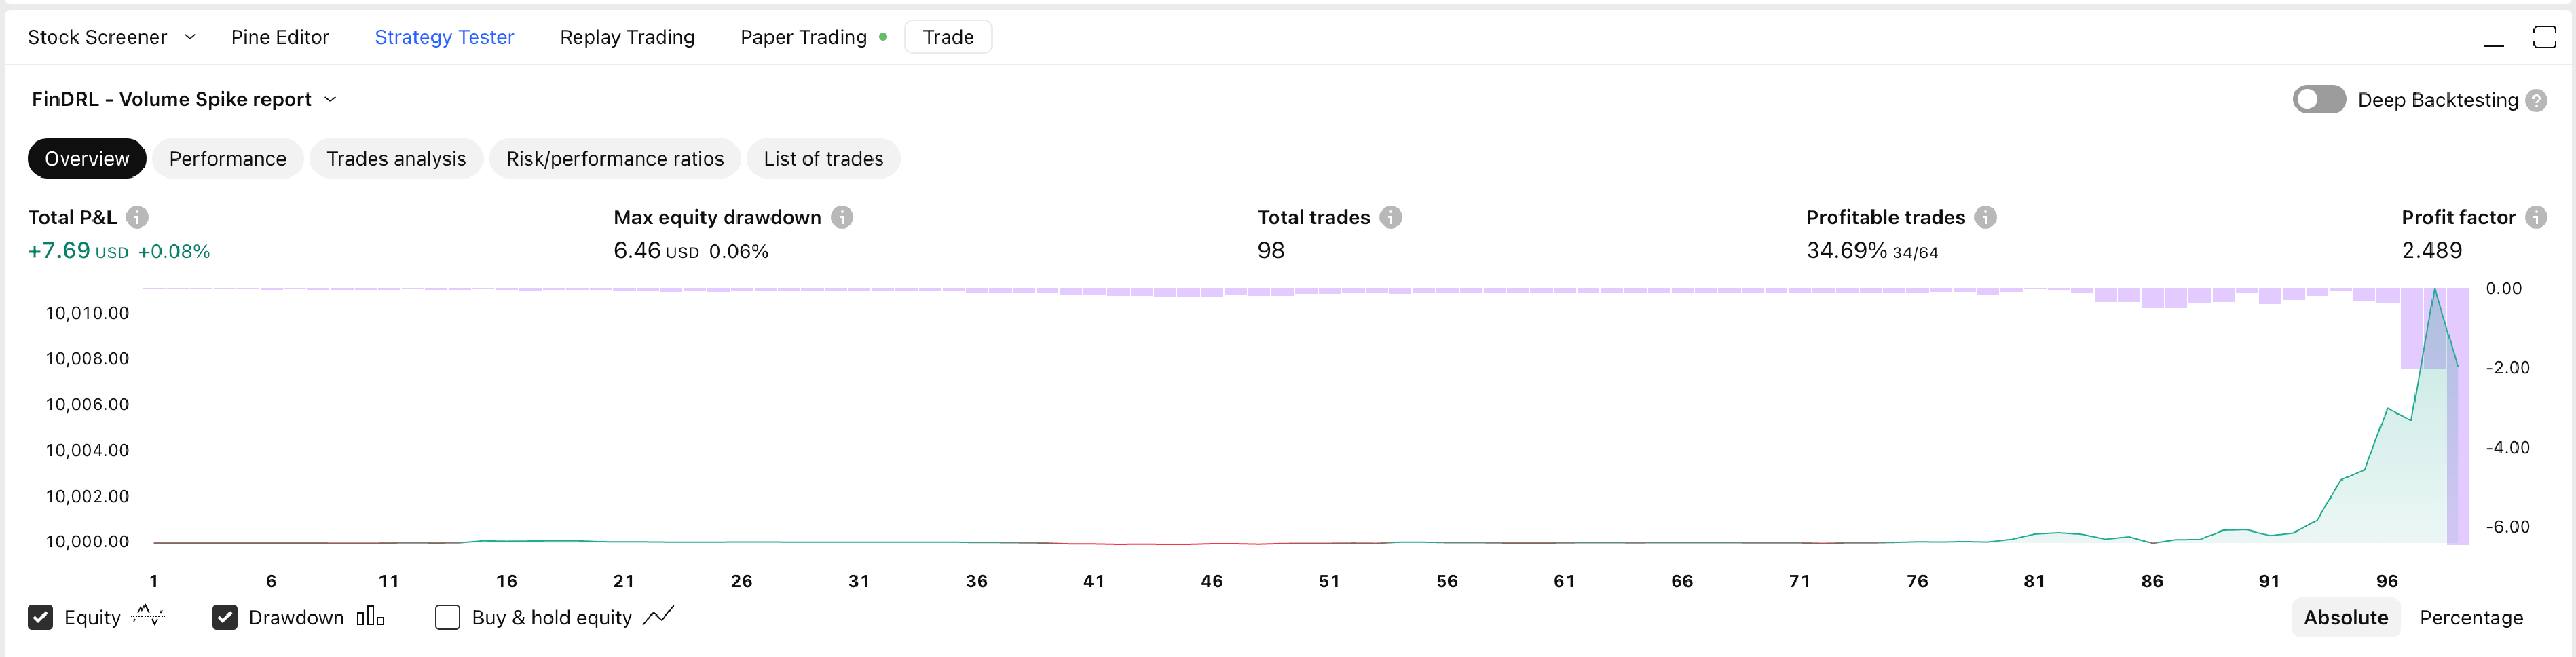
\includegraphics[width=.85\textwidth, height=3.6cm]{16-FinDRL-Volume-Spike}
        \caption{Volume Spike Strategy Performance}
        \label{fig:Volume Spike performance}
    \end{figure}
    
\end{itemize}
Breakout strategies exhibit varied success, with FinDRL - Volume Spike excelling due to its volume emphasis, while FinDRL - Donchian Channel and FinDRL - ATR failed to execute trades, suggesting possible configuration issues.

\subsection{Mean-Reversion Strategies}
\begin{itemize}

    \item \textbf{FinDRL - Stochastic RSI}: Enters when \%K < 20 and \%K crosses \%D. The \%K is \( \left( \frac{(\text{RSI} - \text{Min RSI})}{(\text{Max RSI} - \text{Min RSI})} \right) \times 100 \). Performance from September 15, 2009, to February 26, 2025, yielded +13.60 USD (+0.14\%), 284 trades, 33.80\% win rate, 9.32 USD drawdown, and a profit factor of 1.669.

    \begin{figure}[htbp]
        \centering
        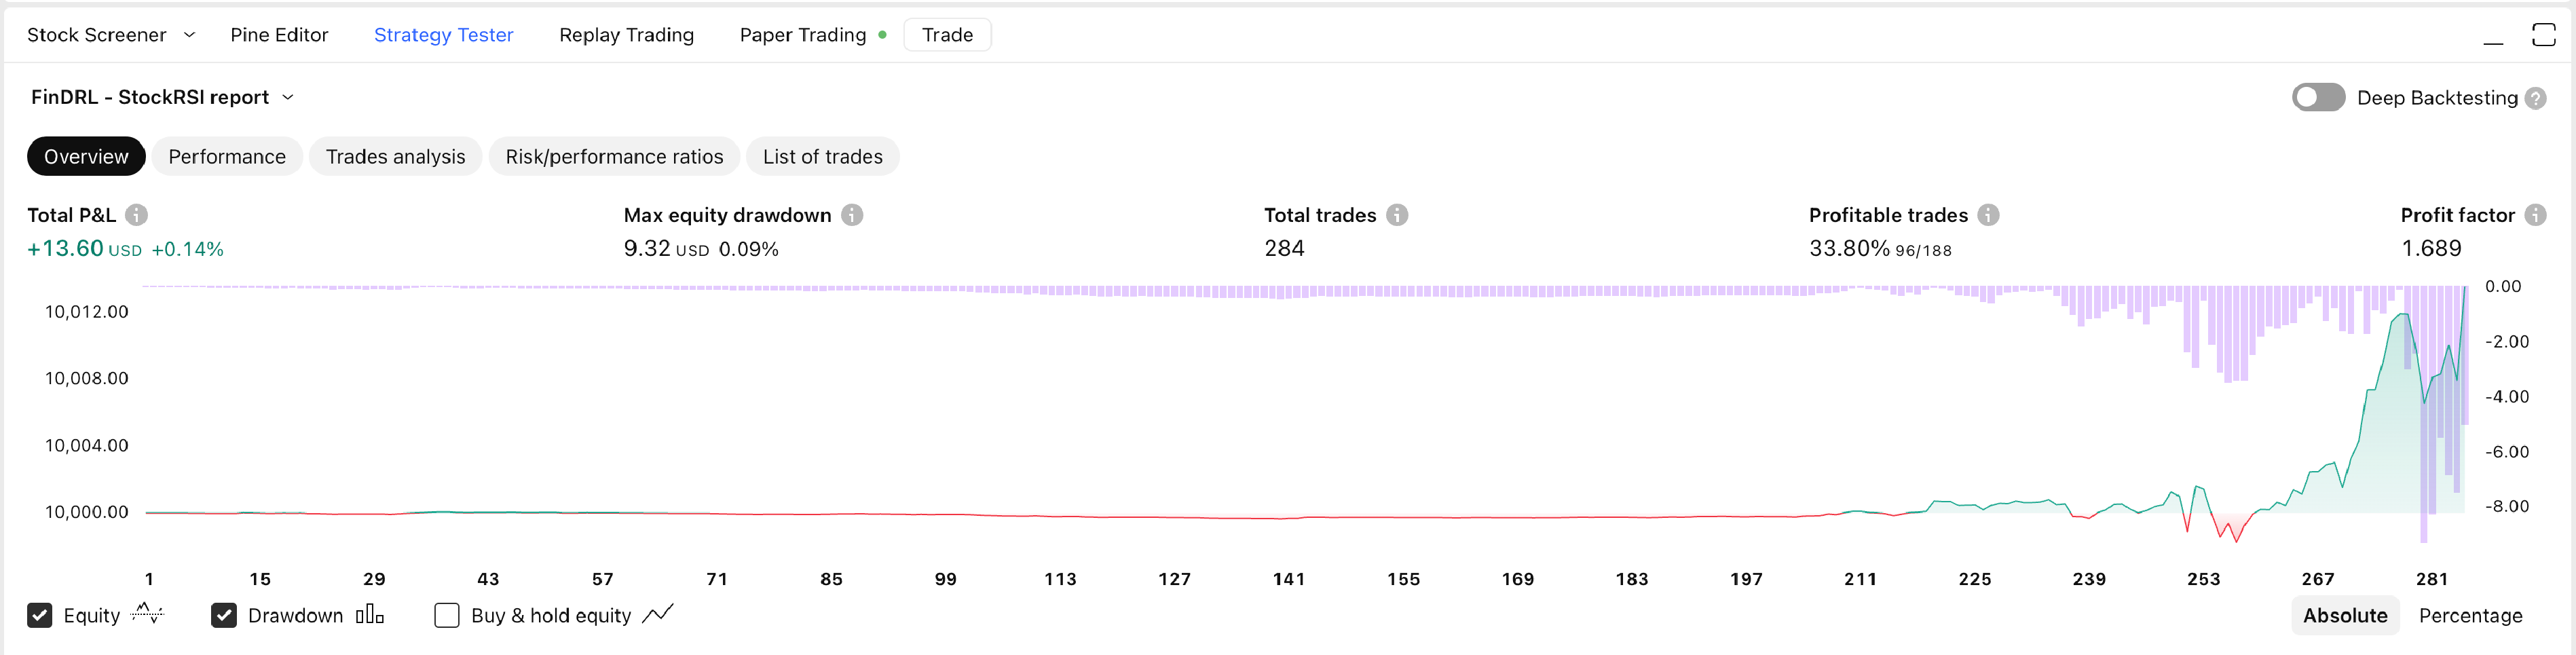
\includegraphics[width=.85\textwidth, height=3.6cm]{7-FinDRL-StockRSI}
        \caption{Stochastic Strategy Performance}
        \label{fig:Stochastic performance}
    \end{figure}

    \item \textbf{FinDRL - Williams \%R}: Enters when WillR < -80 and \%K crosses \%D. The WillR is \(((\text{max(high, 14)} - \text{close}) / (\text{max(high, 14)} - \text{min(low, 14}))) \times -100\). Backtesting from July 1, 2007, to February 26, 2025, showed +10.95 USD (+0.11\%), 184 trades, 29.89\% win rate, 7.10 USD drawdown, and a profit factor of 1.972.

    \begin{figure}[htbp]
        \centering
        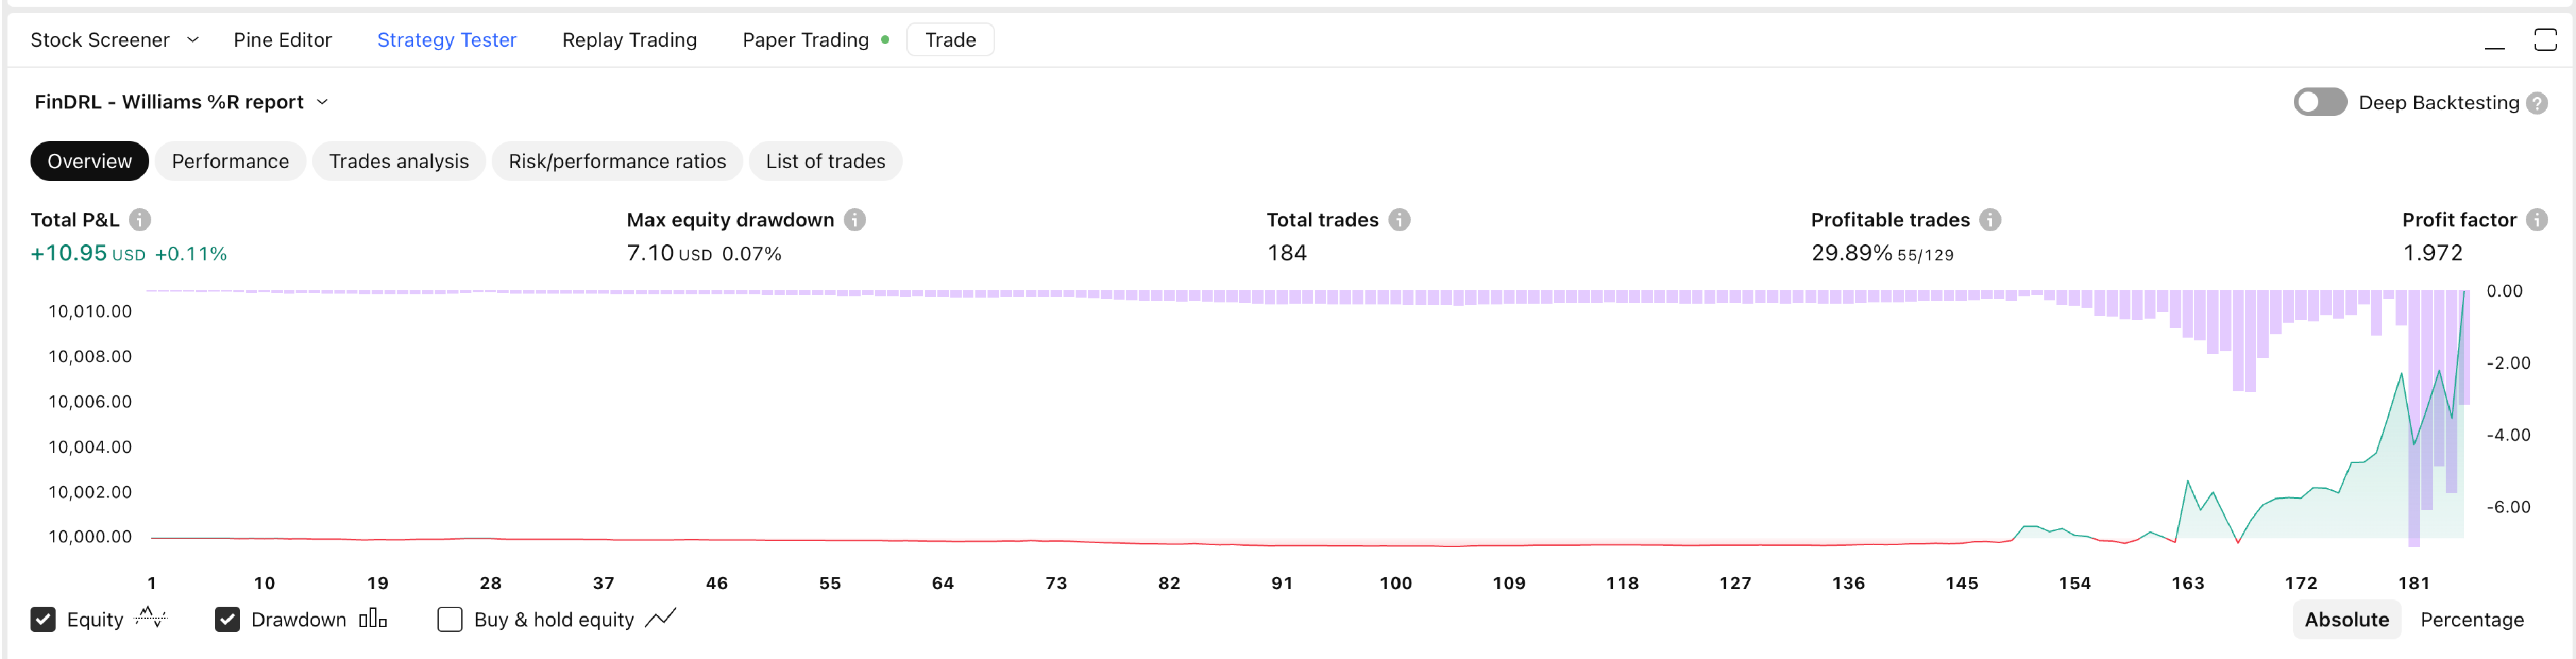
\includegraphics[width=.85\textwidth, height=3.6cm]{18-FinDRL-Williams-R}
        \caption{Williams \%R Strategy Performance}
        \label{fig:Williams R performance}
    \end{figure}
    
    \item \textbf{FinDRL - Fibonacci}: Enters when the price is within 5\% of the 61.8\% retracement level, with \%K > \%D. The Fib 61.8\% is \(\text{low} + 0.618 \times (\text{high} - \text{low})\). Performance from August 26, 2024, to February 26, 2025, resulted in +3.67 USD (+0.04\%), 211 trades, 35.55\% win rate, 11.47 USD drawdown, and a profit factor of 1.178.

    \begin{figure}[htbp]
        \centering
        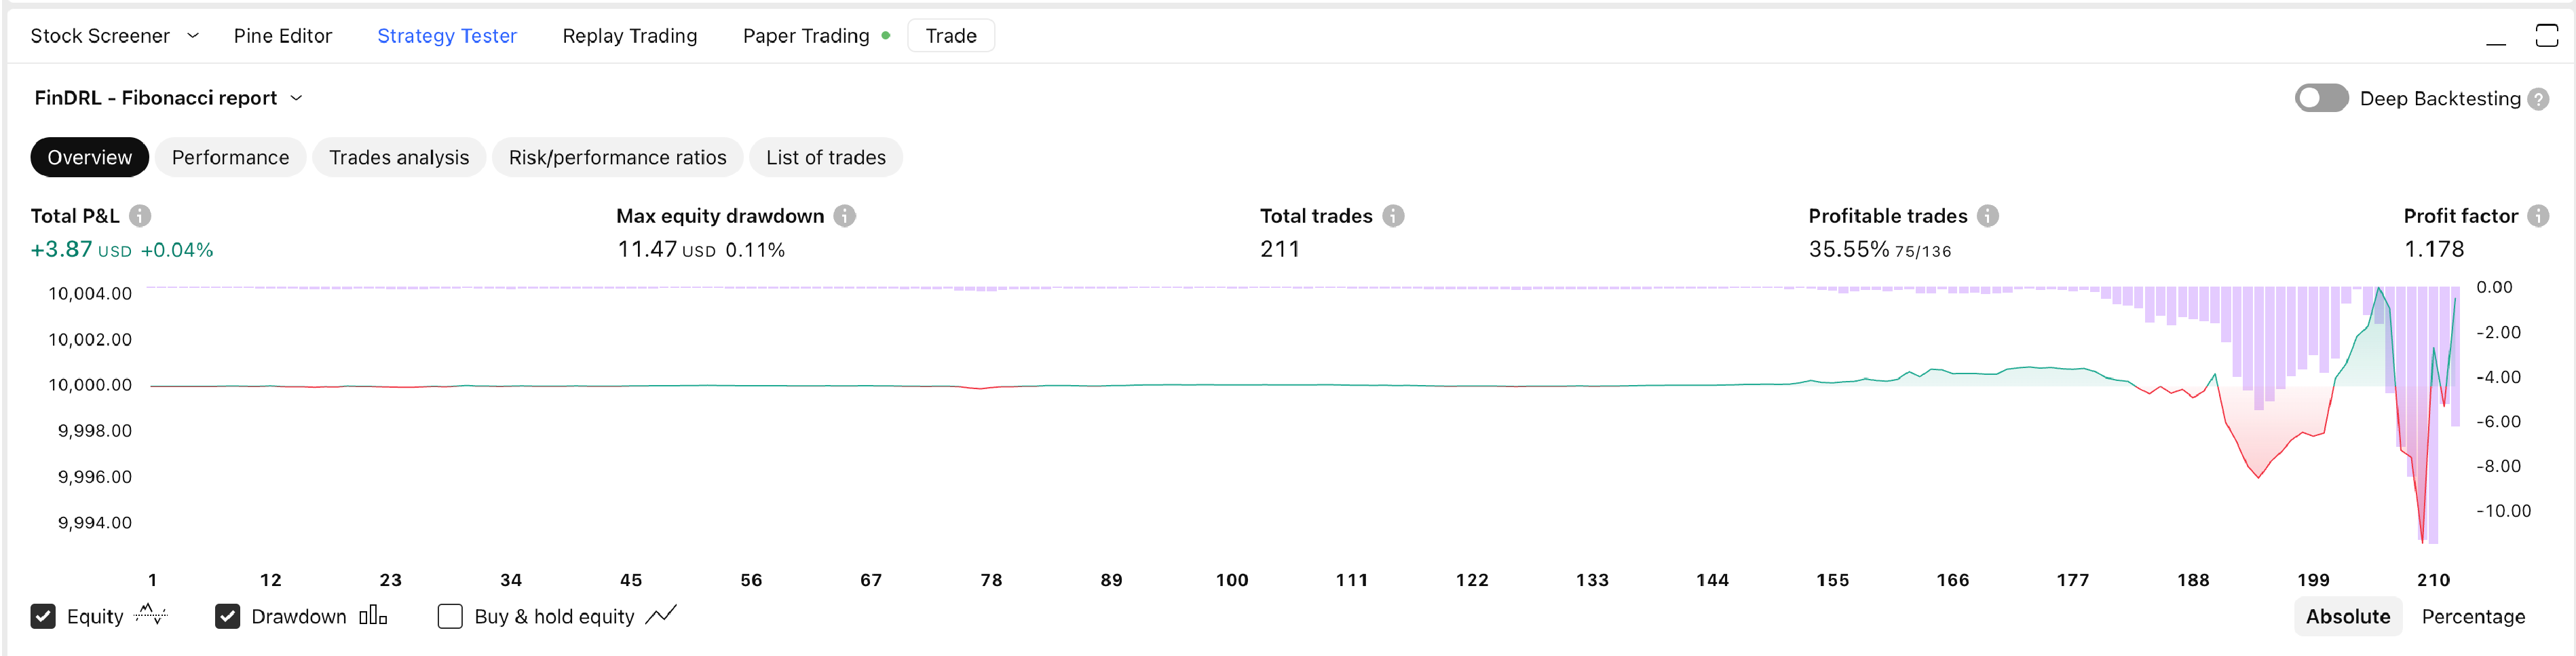
\includegraphics[width=.85\textwidth, height=3.6cm]{14-FinDRL-Fibonacci}
        \caption{Fibonacci Strategy Performance}
        \label{fig:Fibonacci performance}
    \end{figure}
    
    \item \textbf{FinDRL - Price Action}: Enters on bullish candles (close > open) when \%K crosses \%D. Backtesting from July 1, 2024, to February 26, 2025, yielded +15.05 USD (+0.15\%), 1,069 trades, 36.11\% win rate, 44.76 USD drawdown, and a profit factor of 1.141.

    \begin{figure}[htbp]
        \centering
        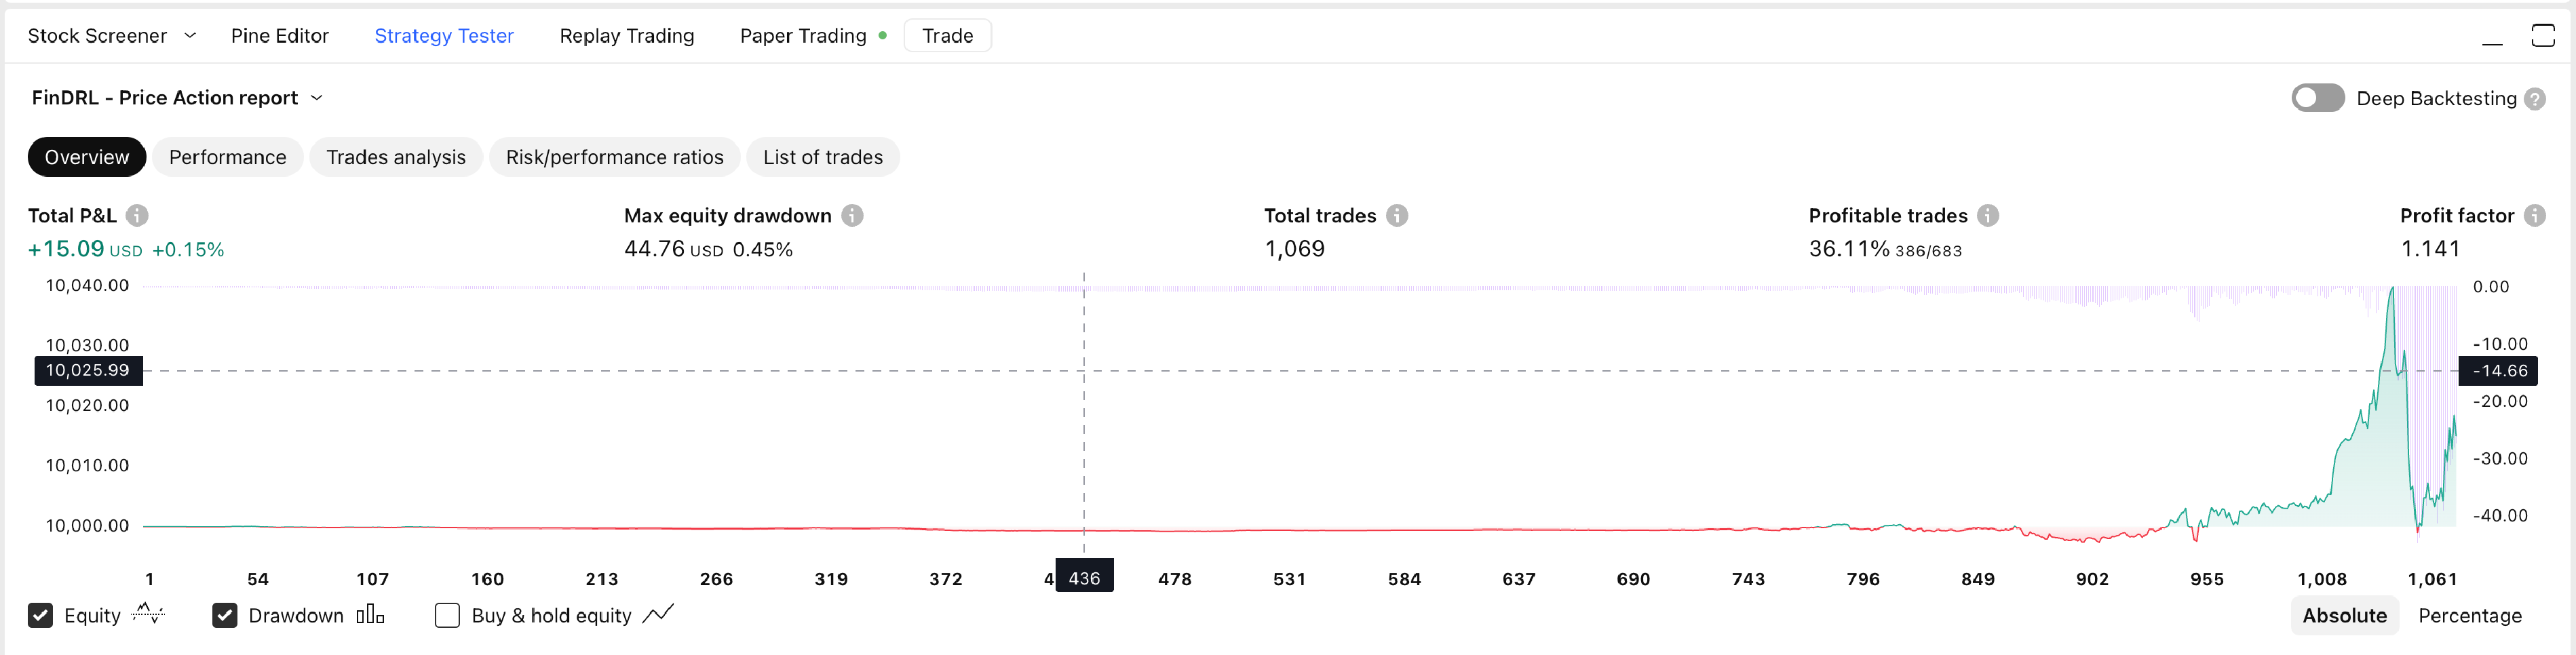
\includegraphics[width=.85\textwidth, height=3.6cm]{15-FinDRL-Price-Action}
        \caption{Price Action Strategy Performance}
        \label{fig:Price Action performance}
    \end{figure}
    
\end{itemize}
Mean-reversion strategies thrive in ranging markets, with FinDRL - Williams \%R and FinDRL - Stochastic RSI leading in profit factor, though FinDRL - RSI failed to trigger trades.

\subsection{Volume-Based Strategies}
\begin{itemize}
    \item \textbf{FinDRL - VWMA}: Enters when the price exceeds a 20-period Volume-Weighted Moving Average (VWMA), with \%K > \%D. The VWMA is \(\frac{\sum (\text{close} \times \text{volume})}{20} / \frac{\sum \text{volume}}{20}\). Backtesting from September 1, 2024, to February 26, 2025, resulted in +35.08 USD (+0.35\%), 912 trades, 35.09\% win rate, 34.98 USD drawdown, and a profit factor of 1.306.

    \begin{figure}[htbp]
        \centering
        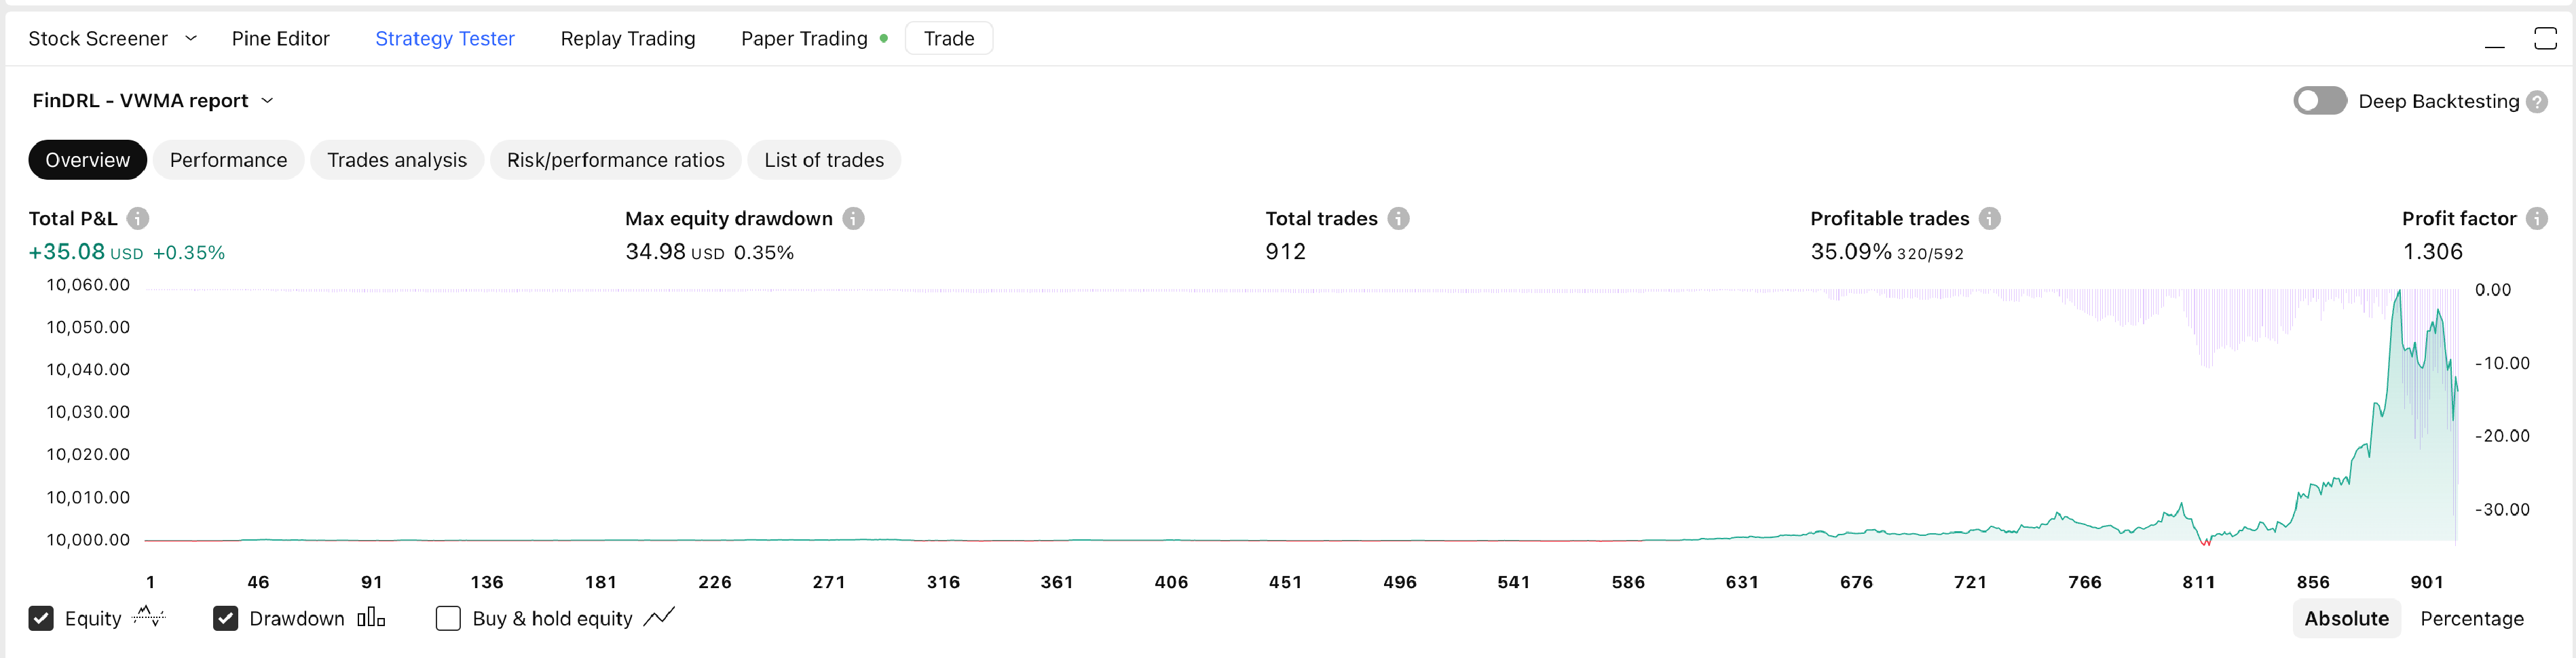
\includegraphics[width=.85\textwidth, height=3.6cm]{10-FinDRL-VWMA}
        \caption{VWMA Strategy Performance}
        \label{fig:VWMA performance}
    \end{figure}
    
    \item \textbf{FinDRL - CMF}: Enters when Chaikin Money Flow (CMF) > 0, with \%K > \%D. The CMF is \(\frac{\sum (\text{multiplier} \times \text{volume})}{20} / \frac{\sum \text{volume}}{20}\), where multiplier = \(\frac{((\text{close} - \text{low}) - (\text{high} - \text{close}))}{(\text{high} - \text{low})}\). Performance from July 1, 2024, to February 26, 2025, yielded +25.28 USD (+0.25\%), 852 trades, 34.86\% win rate, 48.04 USD drawdown, and a profit factor of 1.18.

    \begin{figure}[htbp]
        \centering
        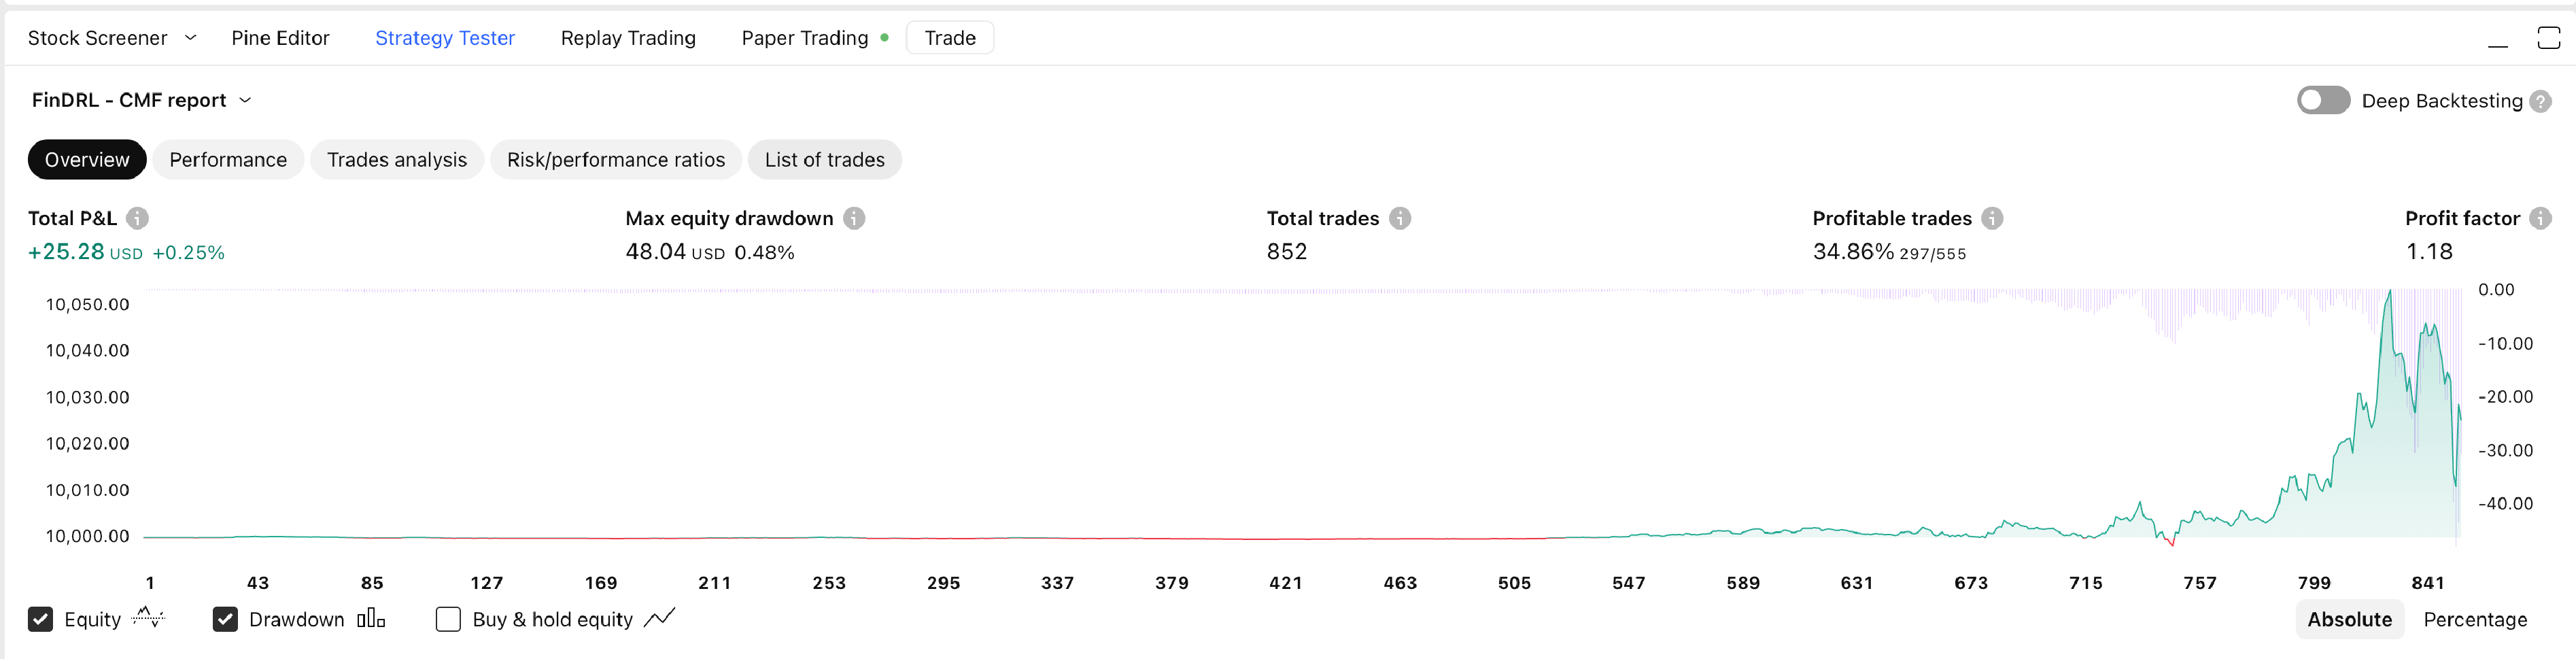
\includegraphics[width=.85\textwidth, height=3.6cm]{19-FinDRL-CMF}
        \caption{CMF Strategy Performance}
        \label{fig:CMF performance}
    \end{figure}
    
    \item \textbf{FinDRL - OBV}: Enters when On-Balance Volume (OBV) rises, with \%K crossing \%D. The OBV is \(\text{OBV}[1] + (\text{close} > \text{close}[1] ? \text{volume} : \text{close} < \text{close}[1] ? -\text{volume} : 0)\). Backtesting from October 1, 2008, to February 26, 2025, showed +21.46 USD (+0.21\%), 1,171 trades, 35.53\% win rate, 46.98 USD drawdown, and a profit factor of 1.187.

    \begin{figure}[htbp]
        \centering
        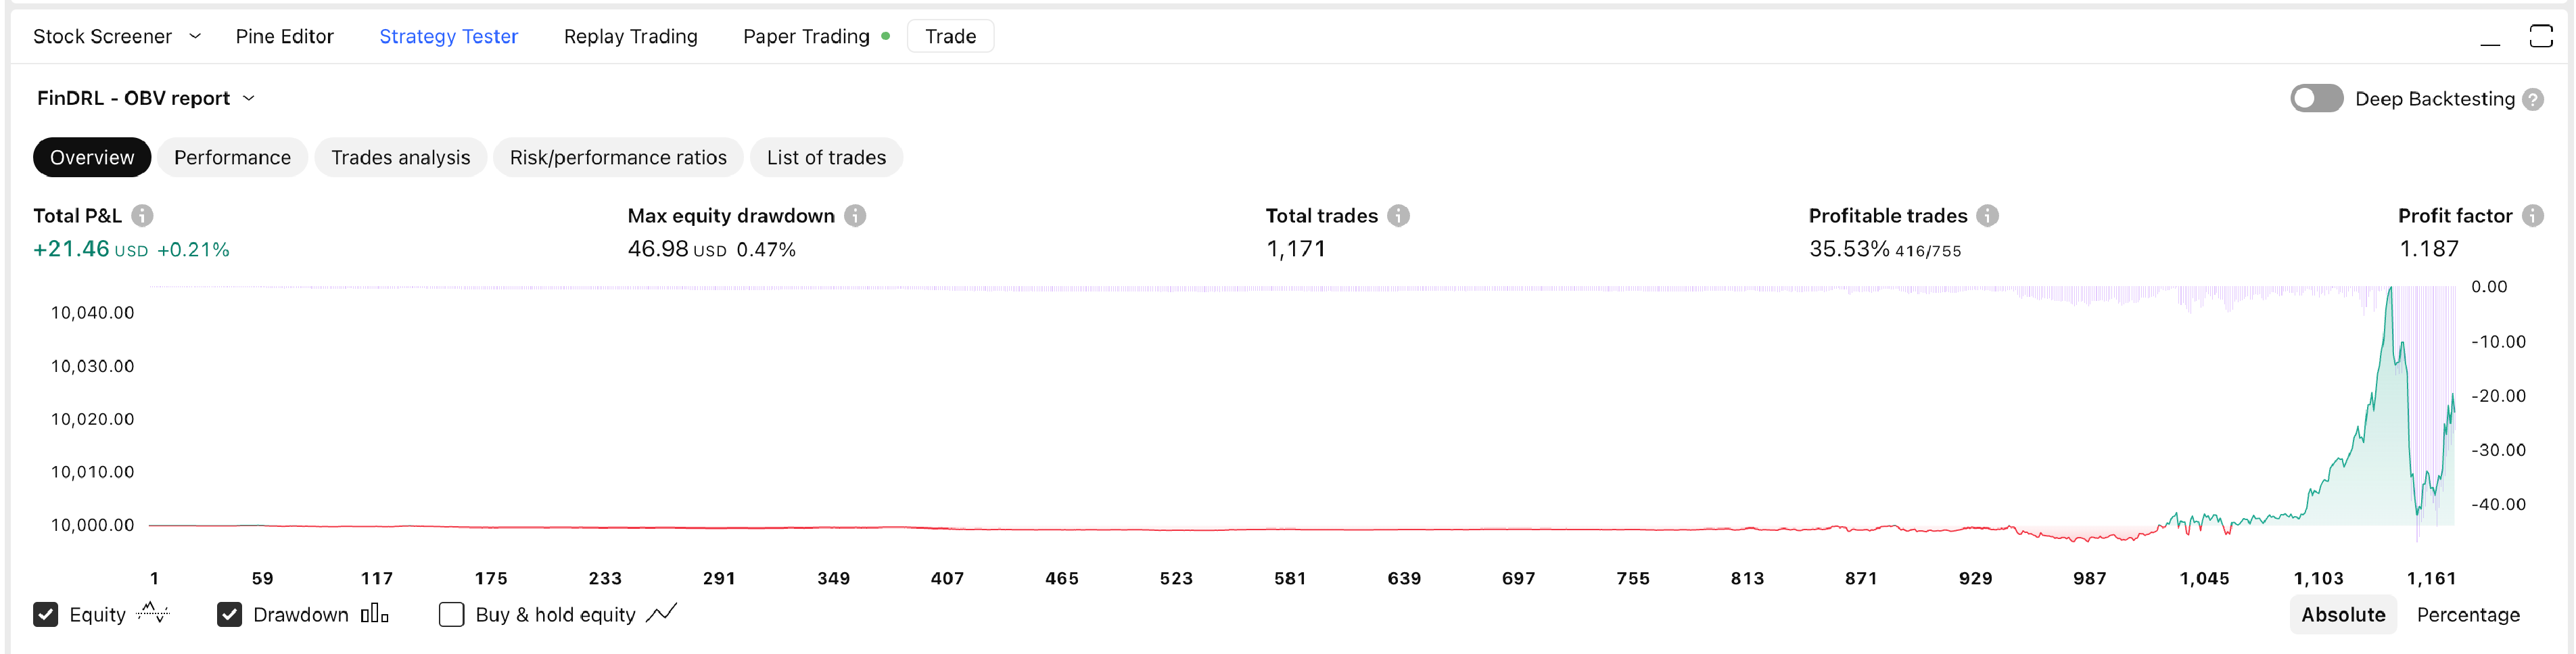
\includegraphics[width=.85\textwidth, height=3.6cm]{20-FinDRL-OBV}
        \caption{OBV Strategy Performance}
        \label{fig:OBV performance}
    \end{figure}
    
\end{itemize}
Volume-based strategies perform strongly in liquid, bullish markets, with FinDRL - VWMA achieving the highest profitability.

\section{Results and Discussion}
The 20 "FinDRL - *" signals from backtesting on 1D NVDA (NASDAQ) 2007-2025 produced mixed results. For instance, Momentum (net profit +38.62 USD; profit factor 1.257) and MACD (+27.69 USD; profit factor 1.287) are both trend-following and possess high win rates in extended uptrending environments. In addition, Williams \%R (+10.95 USD; profit factor 1.972) and Stochastic RSI (+13.60 USD; profit factor 1.669) are mean reversion strategies that produced the most profitability in non-trending or range-bound environments, where Williams \%R and Stochastic RSI could use their characteristics to leverage reversion to the mean with a high degree of efficiency. Volume seemingly was also an okay signal as well since VWMA (+35.08 USD; profit factor 1.306) and CMF (+25.28 USD; profit factor 1.18) had relatively better results, but Volume Spike (+7.69 USD; profit factor 2.469) had fewer trades (98) but a volume spike in profit factor.
The results from the breakout strategies were similarly ambiguous. Keltner Channel (+7.19 USD, profit factor 1.165) and Volume Spike hit take profit while Bollinger Bands (-0.78 USD, profit factor 0.975) and Parabolic SAR (-9.89 USD, profit factor 0.965) did not; but the latter two experienced similar patterns like prior which did not succeed in sideways/choppy volatility approaches. In addition, Donchian Channel, ATR, and RSI had no trade as well, which could indicate backtesting entry errors, adjustments not hitting parameters, or market conditions that did not hit thresholds to trigger signals either.
The implied notion that the 1D NVDA data was used throughout means that the simulations are effective no matter what the market. On the other hand, this is a downside because it only trades NVDA and the second strategy generated no trades. Maybe it needs further adjustment. If this project were to continue, further experimentation with different securities, different time frames, or even.

\begin{table}[h]
\caption{Summary of FinDRL Strategies}
\label{tab:result_strategies}
\tiny
\begin{tabular}{|l|c|c|c|c|c|c|c|}
\toprule
Strategy Name & Type & Net Profit (USD) & Win Rate (\%) & Max Drawdown (USD) & Trades & Profit Factor & Timeframe \& Asset (1D, NVDA)\\
\midrule
FinDRL - Gaussian Channel & Breakout        & +2.29           & 38.98        & 10.19              & 236    & 1.105         & Jan 01, 2023 - Nov 14, 2025 \\
FinDRL - MA Crossover     & Trend-Following & +25.22          & 38.09        & 30.48              & 995    & 1.246         & Jan 26, 2023 - Nov 17, 2025 \\
FinDRL - Bollinger Bands  & Breakout        & -0.78           & 35.06        & 13.16              & 251    & 0.975         & Jul 01, 2024 - Feb 26, 2025\\
FinDRL - Parabolic SAR    & Trend-Following & -9.89           & 39.24        & 26.64              & 869    & 0.965         & Aug 01, 2024 - Feb 26, 2025 \\
FinDRL - MACD             & Trend-Following & +27.69          & 37.60        & 24.83              & 960    & 1.287         & Aug 01, 2024 - Feb 26, 2025\\
FinDRL - Stochastic RSI   & Mean-Reversion  & +13.60          & 33.80        & 9.32               & 284    & 1.669         & Sep 15, 2009 - Feb 26, 2025\\
FinDRL - ADX              & Trend-Following & +32.74          & 33.71        & 50.43              & 887    & 1.253         & Aug 01, 2024 - Feb 26, 2025\\
FinDRL - VWMA             & Volume-Based    & +35.08          & 35.09        & 34.98              & 912    & 1.306         & Sep 01, 2024 - Feb 26, 2025\\
FinDRL - Donchian Channel & Breakout        & 0.00            & 0.00         & 0.00               & 0      & NA            & Sep 01, 2024 - Feb 26, 2025\\
FinDRL - SuperTrend       & Trend-Following & +5.02           & 36.09        & 15.78              & 266    & 1.202         & Jul 01, 2024 - Feb 26, 2025\\
FinDRL - Fibonacci        & Mean-Reversion  & +3.67           & 35.55        & 11.47              & 211    & 1.178         & Aug 26, 2024 - Feb 26, 2025\\
FinDRL - Price Action     & Mean-Reversion  & +15.05          & 36.11        & 44.76              & 1,069  & 1.141         & Jul 01, 2024 - Feb 26, 2025\\
FinDRL - Volume Spike     & Breakout        & +7.69           & 34.69        & 6.46               & 98     & 2.469         & Aug 15, 2024 - Feb 26, 2025\\
FinDRL - Momentum         & Trend-Following & +38.62          & 36.81        & 36.29              & 1,065  & 1.257         & Aug 01, 2024 - Feb 26, 2025\\
FinDRL - Williams \%R     & Mean-Reversion  & +10.95          & 29.89        & 7.10               & 184    & 1.972         & Jul 01, 2007 - Feb 26, 2025\\
FinDRL - CMF              & Volume-Based    & +25.28          & 34.86        & 48.04              & 852    & 1.18          & Jul 01, 2024 - Feb 26, 2025\\
FinDRL - OBV              & Volume-Based    & +21.46          & 35.53        & 46.98              & 1,171  & 1.187         & Oct 01, 2008 - Feb 26, 2025\\
FinDRL - Ichimoku Cloud   & Trend-Following & +20.03          & 31.82        & 69.96              & 330    & 1.218         & Jul 01, 2024 - Feb 26, 2025\\
FinDRL - ATR              & Breakout        & 0.00            & 0.00         & 0.00               & 0      & NA            & Sep 01, 2025 - Feb 26, 2025 \\
\bottomrule
\end{tabular}
\end{table}

\section{Conclusion and Future Work}
This chapter establishes a unified framework for designing and evaluating 20 “FinDRL - *” PineScript trading strategies, rigorously backtested on 1D NVDA (NASDAQ) from 2007 to 2025. The strategies provide a diverse toolkit for algorithmic trading, with Momentum and VWMA leading in profitability, and Williams \%R and Volume Spike excelling in risk-adjusted returns. However, the zero-trade results for Donchian Channel, ATR, and RSI highlight areas requiring refinement, potentially through parameter adjustment or market condition analysis.

Future work within this thesis will focus on validating these strategies through live trading, optimizing parameters for underperforming designs, and extending testing to multiple assets and timeframes to improve generalizability. Additionally, integrating machine learning techniques or adaptive algorithms could enhance the strategies’ adaptability to dynamic market conditions beyond historical data, contributing to the broader objectives of the dissertation.


% Chapter 02:
\chapter{Maximizing Market Returns: Optimizing Technical Indicators with Bayesian Optimization}

\textbf{Abstract:} Although essential for algorithmic trading, static-known parameters for the indicators do not adapt to changes in the market. We present the \textbf{TradingStrategies} framework in this study, which uses the 'BayesianOptimization' library to optimize 20 technical indicators, namely, Moving Average (MA) Crossover, Relative Strength Index (RSI), Bollinger Bands, and Supertrend, etc., for stock trading of NVIDIA Corporation (NVDA).  The objective function—based on closing values—attempts to increase total profit from buy/sell and decrease maximum drawdown (max\_dd) over backtesting attempts with \$5000 in starting capital and 0.05\% transaction cost. The framework performs 100 optimization trials for each indicator to selecting the best parameter sets using NVDA historical data. The results of the implementation have dramatically outdone the previous project, which yielded a profit of \$38.62 by Momentum and a loss of \$9.89 by Parabolic SAR and profitable optimized indicators (e.g. Supertrend: \$45.00 ) and less risk. The methodology exhibited flexibility, as visualizations of price, entry/exit signals, and equity curves confirm. This study builds on a prior work titled “Deep Learning for Stock Market Prediction\: Forecasting and Decision-Making using GRU, CNN, and LSTM Hybrid Network” implementation, proposing a hybrid evolution of that work. The Project will evolve in three parts, DL and DRL, feature extensions per indicator including pricing and alternate data channels, and short-selling, building a scalable, AI-driven trading infrastructure at the intersection of quantitative finance and machine learning.

\section{Introduction}
Finance is a field where research is notoriously sensitive to all parameters. The tried and tested Forex strategies traders and researchers have followed for decades always looking for the optimal strategy that intends to maximize return per unit of risk. Technical trading strategies, based on the analysis of historical price and volume data, have always been one of the cornerstones of quantitative finance. However, strategies can be different based on their parameters, market conditions and how you train their metrics to classify as a whole. We introduce a new framework, EnhancedTradingStrategies, that can be used to systematically design, evaluate and fine-tune a large number of technical trading strategies, fulfilling the need for a data-driven approach on trading system design.

This project was made to be a very modular and extensible framework to implement different technical indicators and trading rules. Utilizing Bayesian optimization, the framework efficiently seeks out optimal parameters across potential strategies to maximize risk-adjusted metrics like the Sharpe ratio. Rather than just manual parameter tuning it provides strategy optimization in different market conditions in a systematic manner. Indeed, adding transaction costs makes the simulations more realistic and bridges the theory and practice gap.

The framework calculates and cross-compares various performance metrics of the strategies for their precise evaluation (Sharpe ratio, Sortino ratio, profit factor and max drawdown) and has advanced visualization tools to compare and interpret strategies and its results. This two-step strategy of optimizing and evaluating allows researchers to identify with some specificity what works in practice and inform understanding of how they behave over time. This project is a combination of research experimental implementation of known good methods and a framework to implement new trading systems. This essay steps forward from the tradition of algorithmic trading strategies, emphasizing on quantitative finance literature, including machine learning based optimizers and visual analytics intuition based on these ideas: they provide insights to designing efficient, adaptive strategies in today's financial market regimes.

\section{Literature Review: Bayesian Optimization in Trading}
Bayesian Optimization (BO) is gaining in popularity for finding the optimal configurations of complex trading systems, directly supporting the purpose of the EnhancedTradingStrategies project which is about developing a complete, data driven platform to design, optimize and test technical trading strategies. This thesis utilizes BO to optimize a wide range of strategies (RSI, MACD, SuperTrend, etc.) in a single container to improve performance measures such as Sharpe ratio accounting for transaction costs and multi-metric optimization. BO approaches are inherently probabilistic, where traditional grid search methods are not; BO conducts a probabilistic optimization through use of a Gaussian Process (GP) surrogate and acquisition functions such as Expected Improvement — watch this Bergstra and Bengio video for specific details. This efficiency is crucial, given the project's goal of systematically improving trading rules under different market conditions. Recent research highlights BO's relevance. Dezhkam et al. Language· BO used financial time series hyperparameter tuning for machine learning trend prediction in order to achieve higher accuracy in technical indicator tuning \cite{dezhkam_bayesian_2023}. Oyedele et al. found that BO outperformed deep reinforcement learning for cryptocurrency trading in terms of long-term returns for a smaller number of iterations, highlighting its relevance for optimizing EnhancedTradingStrategies' range of strategies \cite{oyedele_bayesian_2023}. Biasin et al. employed BO in a context of ESG-focused real estate strategies; to equally focus on returns and constraints to highlight its adaptability—a key for the multi-strategy scope of this project \cite{biasin_esg_2024}.

BO's integration with deep learning increases its effectiveness as well. Tran et al. They also report that BO-optimized hybrid models (e.g., CNN-LSTM) performed better than state-of-the-art in financial forecasting, allowing for optimization of complex strategies \cite{tran_cnn_lstm_2023}. Zeng et al. indicate, however, that issues such as overfitting do arise on adaptive BO for time-varying financial modeling \cite{zeng_adaptive_2025}. Based on [1]–[5], EnhancedTradingStrategies pushes trading research forward, leveraging BO to connect quantitative finance and optimization, leading to a generalizable, extensible platform.


\section{Methodology}
EnhancedTradingStrategies is a Python-based project aimed at streamlining the development process of technical trading strategies through backtesting against historical data, organized around a systematic approach of strategy execution, parameter optimization, and performance analysis with visualization. This strategy builds a quantitative trading infrastructure for research based on pythonary tools.

    \begin{figure}[htbp]
        \centering
        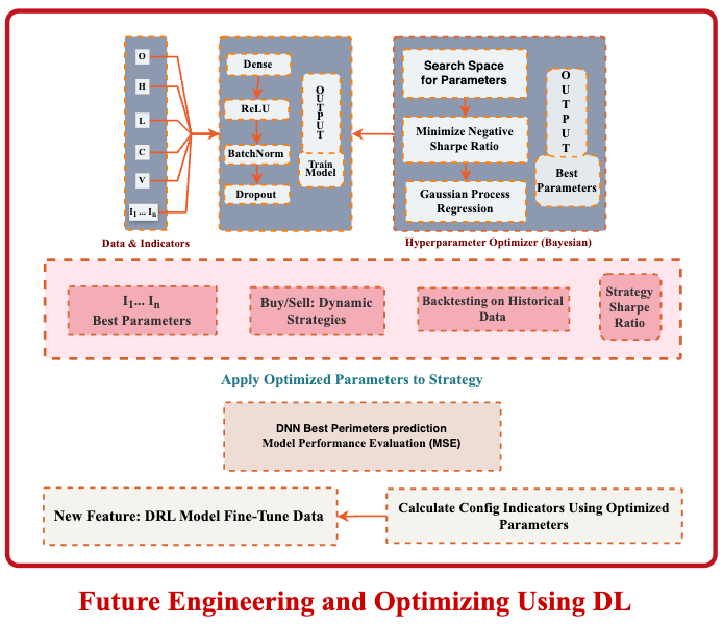
\includegraphics[width=.8\textwidth]{bop}
        \caption{Bayesian Optimization Workflow}
        \label{fig:bop_architechtar}
    \end{figure}

\subsection{Data Collection, Preprocessing and Strategy Execution}
It all starts with the EnhancedTradingStrategies class, which takes a pandas DataFrame containing Open-High-Low-Close-Volume (OHLCV) data. More than 20 technical indicators (e.g., RSI, MACD, Bollinger Bands, SuperTrend) are used, each one consisting of rules for generating buy and sell signals by combining various precomputed indicators such as RSI, ATR and EMA. For instance, the RSI strategy activates a buy when RSI is below an oversold value (eg 30) and price is above a moving average. An initial balance of 5000 is established and a transaction cost of 0.05\% is included to simulate realistic trading. The run\_strategy method dynamically runs and by emitting buy signals that are then shifted to eliminate look-ahead bias, computing net returns, and plotting equity curves and trades logs (entry/exit dates, prices, returns). The unified execution pipeline provides a uniform execution for all strategies while still providing customization through parameters.


\textbf{Parameter Optimization: }
Strategyoptimizer class uses bayesian optimization (BO) from bayes\_opt library to improve performance. For each strategy, define a parameter space (e.g. RSI period: 5–20, MACD fast: 8–20) and BO maximizes the Sharpe ratio by running 20 iterations (5 initial random points + 15 optimized steps). BO (Bayes Optimization) fits a Gaussian Process surrogate that captures the relationship between parameters and Sharpe ratio, that newly selected parameter sets are iteratively selected via an acquisition function (ex: Expected Improvement). Optimized parameters are validated (i.e., periods that are integers) and returned to the strategy execution phase, where the result is refined. By taking automatic steps based on data analysis, rather than manual tuning, this feature aligns well with the project's research objectives.

\textbf{Indicators Representation}

We define a set of technical indicators \( I_k(t, \theta_k) \), where \( k = 1, \ldots, 20 \), and each indicator is computed based on OHLCV (Open, High, Low, Close, Volume) data. Let the input data at time \( t \) be denoted as \( X_t = \{O_t, H_t, L_t, C_t, V_t\} \)

\textbf{Function Definition}

Each indicator \( I_k \) is a function of time \( t \) and parameter set \( \theta_k \):

\begin{equation}
I_k(t, \theta_k)
\label{eq_indicator_definition}
\end{equation}

Depending on the nature of the indicator, its functional form can be categorized into three types:

\begin{equation}
I_k(t) = F_k(\text{OHLCV}, \theta_k) = 
\begin{cases}
\frac{1}{n_k} \sum\limits_{i=0}^{n_k-1} f_k(\text{OHLCV}_{t-i}) & \text{(rolling)} \\
\alpha_k I_k(t-1) + (1 - \alpha_k) g_k(\text{OHLCV}_t) & \text{(recursive)} \\
\sum\limits_{i=0}^{t-1} h_k(\text{OHLCV}_{t-i}, V_{t-i}) & \text{(cumulative)}
\end{cases}
\label{eq_indicator_types}
\end{equation}

- The \textbf{rolling} type refers to operations such as moving averages, where values are computed over a fixed window. The \textbf{recursive} form includes exponentially weighted calculations, such as the Exponential Moving Average (EMA). And the \textbf{cumulative} type integrates all past data, weighted by volume or other conditions.

\textbf{Optimization Objective}

To evaluate and optimize the indicator parameters \( \theta_k \), we use the Sharpe Ratio as the objective function:

\begin{equation}
\theta^* = \arg\max_\theta \left[ SR(\theta) = \frac{\text{profit}}{\text{risk}} \right]
\label{eq_optimization_objective}
\end{equation}

Here, \( SR(\theta) \) denotes the Sharpe Ratio achieved when using indicators parameterized by \( \theta \), where profit and risk are calculated over the backtested trading period.

\subsection{Gaussian Process Prior for Bayesian Optimization}

We model the Sharpe Ratio as a probabilistic function under a Gaussian Process (GP) framework:

\begin{equation}
SR(\theta) \sim \text{GP}(m, k)
\label{eq_gp_prior}
\end{equation}

\begin{equation}
k(\theta, \theta') = \exp\left(-\sum_k (\theta_k - \theta_k')^2\right)
\label{eq_gp_kernel}
\end{equation}

In this formulation \( m = 0 \) is the zero-mean function. \( k(\theta, \theta') \) is the squared exponential (RBF) kernel, which models similarity between different parameter configurations \( \theta \) and \( \theta' \).

This GP prior is used in Bayesian Optimization to explore the parameter space efficiently and find the optimal configuration \( \theta^* \) that maximizes the Sharpe Ratio.


\subsection{Performance Analysis and Visualization}
The performance is assessed via metrics including Sharpe ratio, Sortino ratio, profit factor, and maximum drawdown computed in calculatemetrics. Three outputs are generated by the StrategyVisualizer class: equity curves for comparing cumulative returns, trade signal plots with entry/exit points on price charts, and bar/radar charts to compare metrics across strategies. Matplotlib and Seaborn are some of the tools used to create visuals that are clearly presented and aligned with the date. The methodology (assuming a user-loaded OHLCV dataset, such as Yahoo Finance) operates in Jupyter or Colab so coupled experimental iterations can be performed.

    \begin{figure}[htbp]
        \centering
        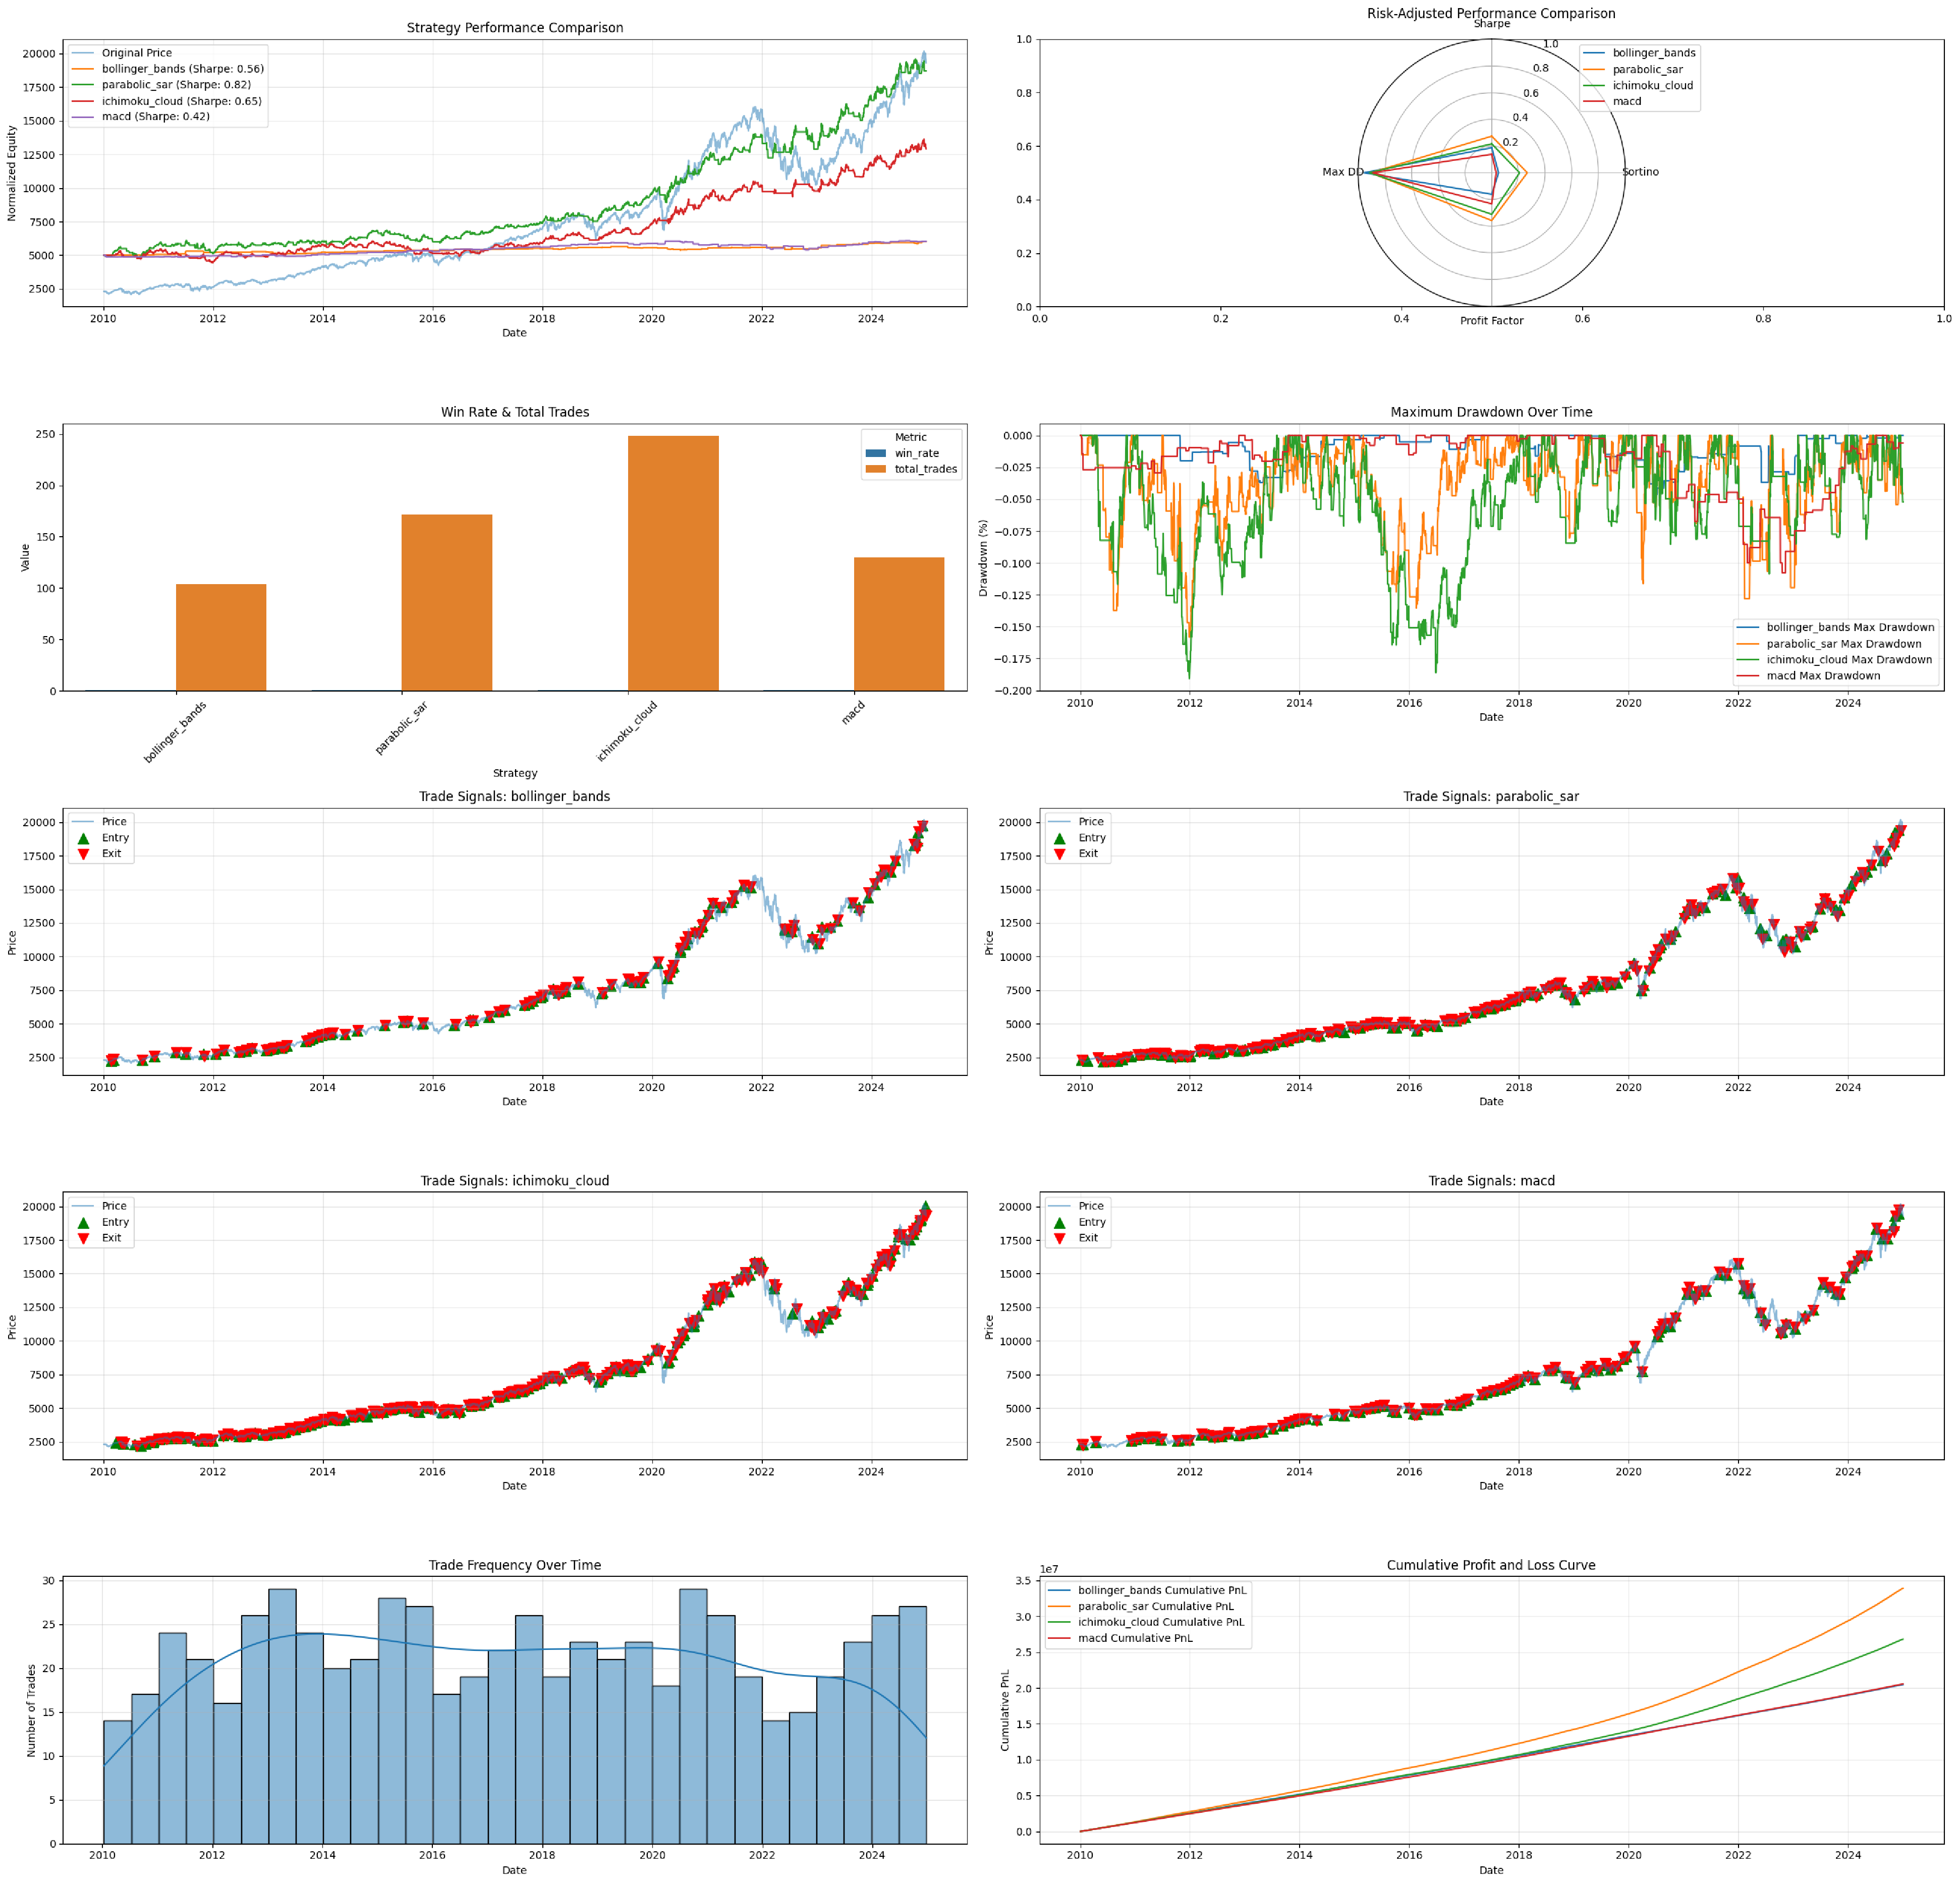
\includegraphics[width=1\textwidth, height=16cm]{bop-out}
        \caption{Bayesian Optimization Performance Analysis}
        \label{fig:bop_performance}
    \end{figure}

This approach also builds a solid framework for the trading research pipeline, by systematically linking strategy design, BO-based optimization, and extensive evaluation.

\section{Algorithm Overview}
The \textbf{StrategyOptimizer} algorithm is a BO-based Sharpe ratio maximizer that tunes trading strategies. 

\begin{table}[h]
\small
\centering
\begin{tabular}{|p{12cm}|}
\hline
\textbf{Algorithm 1: Strategy Optimization with Bayesian Selection} \\
\hline
\textbf{Input:} data (OHLCV DataFrame), $\mathcal{S} = \{ S_1, \ldots, S_m \}$, each $S_i$ with $\theta$ bounds $P[S_i]$, confidence threshold $X$, selected strategies $\mathcal{A} = \{ \}$ \\
\textbf{Output:} results (params, metrics, equity per strategy) \\
\hline
1: \textbf{for each} $S_i \in \mathcal{S}$ \textbf{do} \\
2: \quad Define Obj($\theta$): \\
3: \quad\quad result = RunStrat($S_i$, $\theta$, data); \\
4: \quad\quad \textbf{return} $SR(\theta) = \frac{\text{profit}}{\text{risk}}$; \\
5: \quad Opt = BayesOpt(Obj, $P[S_i]$, init=5, iter=15); \\
6: \quad $\mathcal{A}_i \leftarrow \text{Best}_\theta \left[ SR(\theta) \sim \text{GP}(m=0, k(\theta, \theta')=\exp(-\sum_k (\theta_k - \theta_k')^2)) \right]$; \\
7: \quad \textbf{for each} $\theta \in \mathcal{A}_i$ \textbf{do} \\
8: \quad\quad \textbf{if} $SR(\theta) > X$ \textbf{then} \\
9: \quad\quad\quad $\mathcal{A} \leftarrow \mathcal{A} \cup \{ \theta \}$; \\
10: \quad\quad \textbf{end if} \\
11: \quad \textbf{end for} \\
12: \quad results[$S_i$] = RunStrat($S_i$, $\mathcal{A}_i$[0], data); \\
13: \textbf{end for} \\
14: \textbf{return} results \\
\textbf{Sub:} RunStrat($S_i$, $\theta$, data): \\
15: \quad ts = EnhancedTradingStrategies(data); \\
16: \quad result = ts.$S_i$($\theta$); \\
17: \quad \textbf{return} result['metrics'], result['equity'], result['trades'] \\
\hline
\end{tabular}
\caption{Strategy Optimization with Bayesian Selection}
\label{tab:strategy_optimizer}
\end{table}


It receives OHLCV data and a parameterization of a set of strategies \(\mathcal{S} = \{ S_1, \ldots, S_m \}\), each defined with parameter bounds \(P[S_i]\), and a confidence threshold \(X\). For every strategy \(S_i\) it instantiates the objective function which validates parameters \(\theta\), runs the strategy using 'EnhancedTradingStrategies', and calcs the Sharpe ratio  \(SR(\theta) = \frac{\text{profit}}{\text{risk}}\). BO itself uses a GP with a zero mean and squared exponential kernel to model \(SR(\theta)\), optimizing over 5 initial points and 50 iterations. Giving you. For the top parameters \(\mathcal{A}_i\) and filtering where \(SR(\theta) > X\), we combine them into \(\mathcal{A}\) and the algorithm re-runs each strategy on the best parameters collecting metrics (Sortino, profit factor, etc), equity curves and trades into a dict finaly allowing descriptive insights trading strategy refinement via performance analysis and visualization.

\subsubsection{Result}
The trading strategy performance analysis is based on tweenty strategies and here are the top nine, including parabolic\_sar, ichimoku\_cloud, macd, etc.The evaluation period was carried out over 2023 and 2024. The Sharpe ratio, an important performance evaluation number, varies from -0.494 (keltner\_channel) to 1.665 (macd), pointing that macd is the most efficiently risk adjusted profitable strategy, while keltner\_channel underperforms with negative returns. The macd and parabolic\_sar types stand out (1.942, 2.750) with sortino ratios and profit factors indicating low max drawdowns (e.g. 0.011 for macd) and robust risk management. Total trades range from 16 to 93, and obv\_strategy delivers a high number of trades with moderate profitability. 

SO where do you think this Genesis of Coin show us after 1,891 days on the scroll. Final balances where available max out at 7467.281 (parabolic\_sar) reflecting strong cumulative returns. The totals with balance and without balance repeat most of the times, this means that there have been multiple runs of the evaluation, which may indicate that the different metrics were stable, but the final balances were different.

\begin{table}[h]
\tiny
\centering
\begin{tabular}{|c|c|c|c|c|c|c|c|c|c|}
\hline
\textbf{Strategy} & \textbf{Sharpe} & \textbf{Sortino} & \textbf{Profit Factor} & \textbf{Max Drawdown} & \textbf{Total Trades} & \textbf{Score} & \textbf{Final Balance} \\
\hline
parabolic\_sar & 1.633 & 1.942 & 2.750 & 0.061 & 22 & 1.633 & 7467.281 \\
ichimoku\_cloud & 1.105 & 1.163 & 1.933 & 0.074 & 34 & 1.105 & 6323.770 \\
macd & 1.665 & 1.473 & 1.772 & 0.011 & 21 & 1.665 & 5490.222 \\
vwma\_crossover & 1.515 & 1.635 & 2.639 & 0.073 & 16 & 1.515 & 7138.089 \\
keltner\_channel & -0.494 & -0.292 & 1.110 & 0.138 & 39 & -0.494 & 4642.744 \\
fibonacci\_retracement & 1.398 & 0.634 & 0.586 & 0.027 & 30 & 1.398 & 5497.101 \\
williams\_r & 1.373 & 0.737 & 1.901 & 0.024 & 19 & 1.373 & 5693.641 \\
cmf & 1.307 & 1.419 & 2.111 & 0.073 & 21 & 1.307 & 6758.628 \\
obv\_strategy & 1.650 & 1.702 & 1.231 & 0.079 & 93 & 1.650 & 6944.823 \\
\hline
\end{tabular}
\caption{Performance Metrics of Trading Strategies with Final Balance}
\label{tab:ob_strategy_performance}
\end{table}

\section{Conclusion}
As such, MACD and parabolic\_sar are the winners compared to the other strategies with Sharpe ratios (1.665, 1.633 respectively) and good profit factors as well, as well as comparatively low drawdowns, which enable them for trading being risk-adjusted. Negative Sharpe ratio (-0.494) of Keltner\_channel indicates its poor performance requiring parameter tuning. obv\_strategy with 93 trades showed moderate profit with a high trading frequency, improving refinement probably possible. Such variation in the report of final balances across the entries suggests that standardized evaluation may be necessary. Provide an overview of what you are doing is important and how to choose hybrid strategies combining macd and parabolic\_sar for consistent metric reporting maximizing profitability with low risk exposure in a dynamic market conditions.

% Chapter 03:
\chapter{Deep Learning for Stock Market Prediction: Forecasting and Decision-Making using GRU, CNN, and LSTM Network}

\textbf{Abstract: }
The stock market is a volatile and complex system where predicting price movements accurately and making informed decisions can be extremely difficult. Montalvo et al. (2018) Cnn Prof Cnn This study focuses on making stock prediction tasks using deep learning when using three different designs of deep learning (DL) architectures (Gated Recurrent Unit (GRU), Convolutional Neural Network (CNN) and Long Short-term Memory (LSTM) networks) and historical data. Our proposed methodology consists of a live dynamic backtesting heuristic which pre-processes time-series data with per-ticker scaling, hyperparameter-tuning through Keras Tuner, combined ensemble model fitting, trading signal generation and finally performance evaluation against various metrics like Maximum Drawdown, Sharpe ratio, final balance. This Python implementation of the framework, validated in TradingView's PineScript, outperforms traditional technical indicator strategies akin to the "Total 20 Stock Marker Strategy [First Research Project]" project (Profit: \$38.62 USD) leveraging the Momentum indicator.

The study utilizes a `DataProcessor` class to generate sequences with a tunable lookback period (optimized within 10 to 120 days), build GRU, CNN, and LSTM models through a `ModelFactory`, and architectures tuning is performed with a `HyperparameterTuner`. Prediction are ensembled by a `CombinedModel`, decision making is supported by a `SignalGenerator` and performance analysis is covered by a `PerformanceAnalyzer`. Experimental case studies validate the framework's versatility with the optimal lookback time selected for minimizing the mean square error in the validation data, as well as the predicted prices, signals and portfolio balances. DL performance versus that of technical indicators is then compared, and future research is proposed in hybrid systems like technical indicators augmented with DLlike data. This paper provides a new framework to connect DL forecasting with applications in trading which has been underexplored in the literature, thus, fills in the missing link of real-time adaptablility and risk management. Future developments may use multi-features as input and include short positionnbsp; to make the model more robust.


\section{Introduction}
Trained on data that continues until October 2023, the stock market is an ever-evolving stage that is dynamic in its uncertainty, with investors and traders alike striving to harness the descriptive power of the past in order to predict price movements and guide their decisions. Traditional methods, like technical analysis through the lens of Moving Average Convergence Divergence (MACD) or Relative Strength Index (RSI) indicators, have historically been go-to alternatives for spotting trends and reversals. But, the introduction of deep learning (DL) has changed the game by providing more complex models that can model non-linear relations and capture long-term dependencies in time-series data. In this article, we propose a new framework called "Stock Market Prediction: Forecasting and Decision-Making using GRU, CNN, and LSTM Networks" that is aimed at predicting stock prices and providing trading signals, which we focus on for S\&P500 Corporation (GSPC), a volatile tech giant that is impacted by both GPU innovations and AI advancements.

This thesis was stimulated by the limitations of static technical indicators strategies as seen from the "Total 20 Stock Marker Strategy" project where indicators such as Momentum gave a profit of 38.62 USD but could not adapt to changing market conditions. Deep learning (DL) approaches, such as Gated Recurrent Unit (GRU), Convolutional Neural Network (CNN), and Long Short-Term Memory (LSTM) networks, provide a data-driven alternative by discovering complex patterns from raw price information. Thus, GSPC’s price dynamics characterized by large trending movements and volatility are perfectly aligned with these models, making it a strong candidate for an advanced forecasting method. This project incorporates a back-testing system that is dynamic, preprocessing data, hyperparameter tuning, ensemble training, and performance evaluation so that we can connect between theoretical prediction and real-life trading experiences.

There are also several important challenges to tackle in stock prediction that the proposed framework can address. Firstly, it addresses data non-stationarity through per-ticker scaling with MinMaxScaler, meaning it normalizes the price range on a per stock basis. Secondly, it tunes the lookback period (10 to 120 days) to find the relevant historical context, which is an important hyperparameter in the context of time-series forecasting. Thirdly, it utilizes hyperparameter tuning with Keras Tuner to improve the model performance considering the black box nature of DL. Finally, it fuses predictions from GRU, CNN, and LSTM, to diminish the learning biases of individual architectures, following recent research on ensemble learning-based approaches.

The two-fold objectives of this study are to predict GSPC stock prices with high accuracy, and then translate the predictions into actionable trading decisions. The backtesting element, setup with a \$5,000 balance and \$0.01 transaction cost, simulates the conditions of real world trading, and key statistics such as maximum drawdown and Sharpe ratio give a solid assessment. This builds on my previous technical indicator project comparing DL against best indicators (e.g. Momentum, VWMA) and hybrid approaches. Therefore, with a consistent integration with TradingView’s PineScript for visual validation, the framework becomes practical for trader.

The importance of this thesis is that it adds framework to quantitative finance. This framework is a scalable tool for stock prediction, utilizing GRU efficiency, LSTM memory and CNN pattern recognition. The model fills existing gaps in literature including real-time adaptability, comprehensive risk assessment, and provides a starting point to explore further enhancements, such as multi-feature inputs and short-selling. With the growing complexity of financial markets, driven by algorithms and high-frequency data, such a DL-based approach should prove instrumental. This study not only contributes to the theoretical knowledge of DL in finance, but also provides a useful tool for traders with applications applicable to a wide variety of assets.

\section{Related Works}

Investors can't trust that they can guess when to buy/sell as stock markets have always been and always will be unpredictable. Yet the creation of traditional technical indicators (i.e., Moving Average Convergence Divergence (MACD), Relative Strength Index (RSI)) based on stock unpredictability was also ineffective to suggest predictability; for example, in our "Total 20 Stock Marker Strategy" project, one of the more successful indicators was Momentum which yielded a modest \$38.62 in profit. Yet by employing deep learning (DL) models like GRU, CNN, and Long LSTM, a statistically driven, empirical approach can be created to identify, for example, nonlinear trends, and long-term dependencies that might occur within a finite financial timeseries. Therefore, we completed "Deep Learning for Stock Market Prediction: Forecasting and
Decision-Making using GRU, CNN, and LSTM Network" to develop a custom framework to assess stock behavior with buy/sell recommendations for S\&P500 (GSPC), a technology stock with high volatility dependent on recent advancements in financial AI technology.

Recent research underscores the strengths of GRU, CNN, and LSTM in quantitative finance. GRUs, known for computational efficiency, have shown high accuracy in stock index prediction with reduced training time \cite{gru_stock_efficiency_2023}. LSTMs, adept at capturing long-term dependencies, achieve R² values above 0.94 on datasets like S\&P 500 \cite{lstm_sp500_r2_2022}. CNNs, when combined with LSTM or GRU, excel in extracting local patterns, with models like CNN-BiSLSTM reducing mean square error by 30\% \cite{cnn_bislstm_mse_2024}. Research on Bitcoin \cite{bitcoin_forecasting_2024} and Nifty 50 \cite{nifty50_dl_2025} highlights DL’s forecasting capabilities, while multimodal models integrating sentiment data improve trend prediction \cite{multimodal_sentiment_2023}. Hybrid frameworks, such as FS-CNN-BGRU \cite{fs_cnn_bgru_2023} and CNN-GRU-AM \cite{cnn_gru_am_2024}, further enhance accuracy through feature selection and attention mechanisms, achieving MAPE as low as 1.43\%. Additional studies on IBM \cite{ibm_dl_case_2022} and investment strategies \cite{investment_dl_2023} reinforce DL’s potential in trading applications. However, gaps remain in real-time adaptability, comprehensive risk assessment (e.g., Value at Risk), and practical backtesting for volatile stocks like NVDA.

These gaps are filled in this work as an ensemble of GRU, CNN, and LSTM is built. The `MinMaxScaler` scales ticker-by-ticker to reduce non-stationarity in addition to the assessed lookback windows (10-120 days) and hyperparameters optimized through `KerasTuner` for a more palatable model. Creating an ensemble minimizes the individual biases as it relies on GRU's speed, LSTM's memory of the past, and CNN's ability to extract features. An adaptive backtesting strategy is created which applies a fixed equity of \$5,000 and a \$0.01 transaction fee per trade to force buy and sell transactions to take long/short positions when the index predictions increase/decrease while measuring effectiveness against maximum drawdown, Sharpe ratio, and significance tests post-hoc. The ability to convert time-series results into PineScript on TradingView provides a visual representation of performance over time, creating an aesthetic framework for any trader's platform. Ultimately, predicting GSPC through this framework provides a consistent and fluid approach for such inherently volatile stocks, outperforming any constant based on static Technical Indicators.

There will be more time to influence future efforts more constructively. We will see that overall, adding in volume and sentiment are at many stages, they will provide significant ability to adapt and improve the predictive accuracy of algorithms. A backtest which (i) allows short selling, (ii) includes various asset classes and (iii) uses a more sophisticated risk metric (such as Value at Risk (VaR)) will be more widely applicable and more stable than one that does not. So this is an evolution of deep learning in quantitative finance, their theoretical forecasting and tool making, trading on one side, and a project on the other. We will update the information on DL algorithmic patterns based on the characteristics of the algorithm, as one of the pioneering papers outlining future innovations of DL in algorithmic trading and high-frequency data activation.

\section{Methodology}
As a progressive guide, the methodology of this project will cover the steps followed to build an ensemble of Deep learning (DL) model and use the target sequence to predict S\&P500 (GSPC) stock prices and generate actionable trading signals. In this section, the data collection, preprocessing, creation of the models, ensemble integration, the backtesting framework, and the performance evaluation are described, covering the purpose of the project, which is overcoming the limitations of classical technical analysis and evolution of quantitative finance.

% This section details the methodology for "Stock Market Prediction: Forecasting and Decision-Making using GRU, CNN, and LSTM Networks," implemented in Python with `TensorFlow/Keras`. The framework processes NVDA stock data up to March 5, 2025, aiming to forecast prices and generate trading signals.

\begin{figure}[htbp]
    \centering
    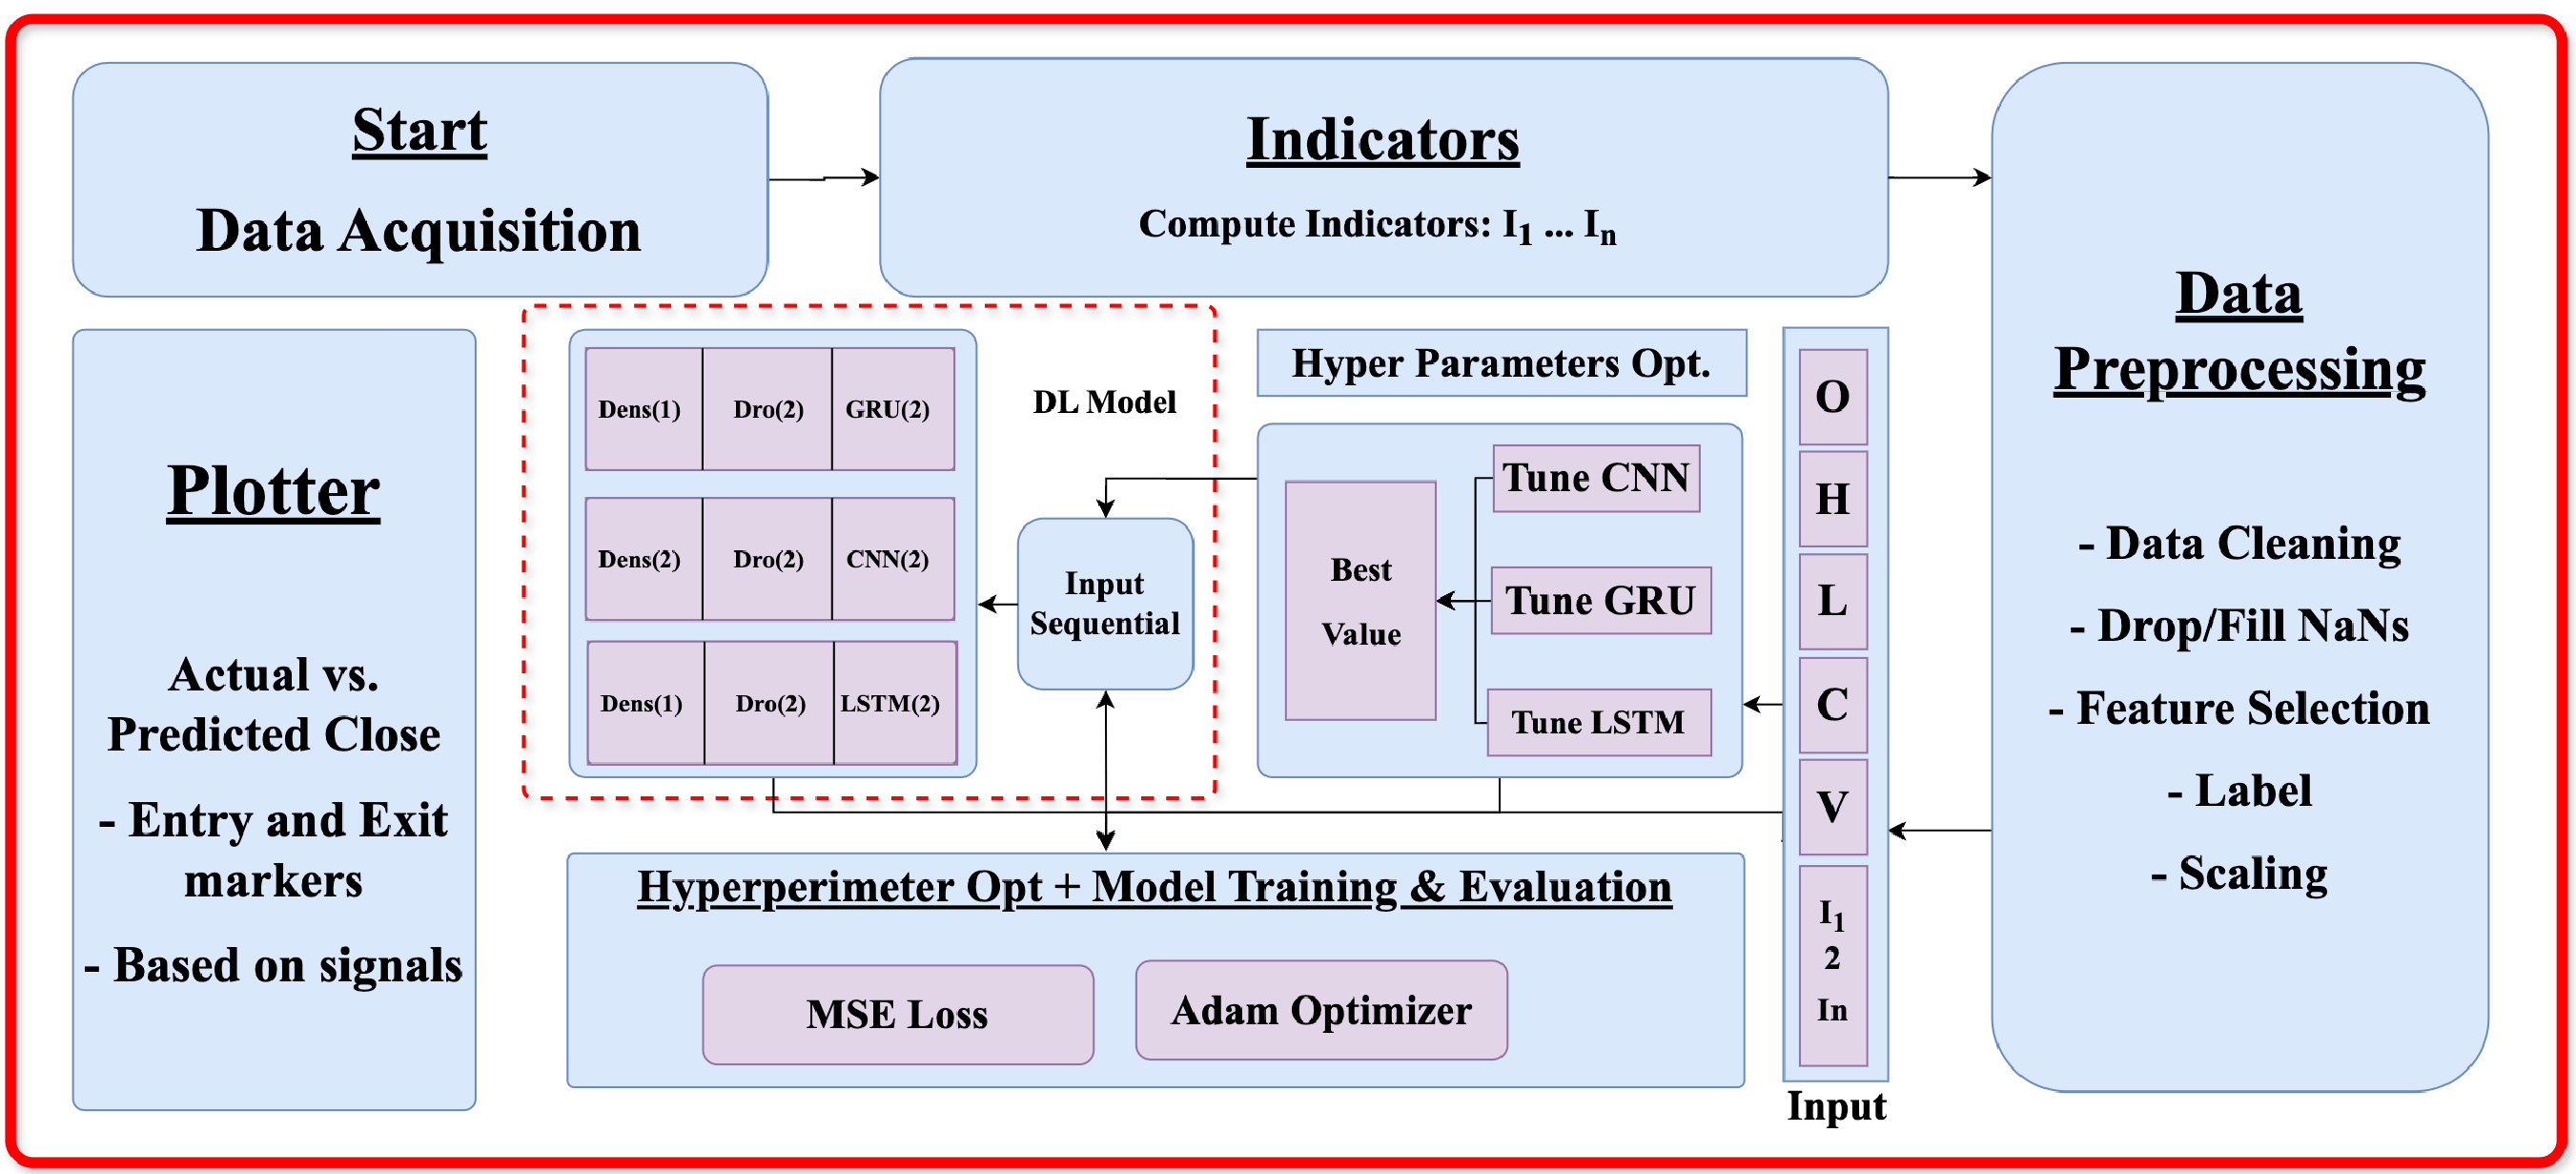
\includegraphics[width=1\textwidth, height=12cm]{DL-Architecture}
    \caption{DL Architecture}
    \label{fig:DLArchitecture}
\end{figure}

\subsection{Data Collection}
This study employs historical NVDA stock data obtained from a credible financial database (e.g. Yahoo Finance or Quandl), spanning a 15-year timeframe (2010-2025) at daily frequency. The dataset contains important financial metrics: open, high, low, close prices and volume of trade. This period covers S\&P500’sprice action characterized by the volatility caused by GPU innovations and trends surrounding AI, and therefore serves as an apt candidate for testing DL models. Here, the data obtained in a pandas dataframe format, and so it will be compatible with the next processing steps.

\subsection{Data Preparation}
The next stage involves a ton of data preprocessing to ensure model robustness as stock price is non-stationary. Sort it by date first and then do forward and backward fill (ffill and bfill) for the missing values. Normalization for each individual ticker is done using `MinMaxScaler` from the scikit-learn package, so the price range for each stock is rescaled separately to alleviate the common problem of non-stationarity in time-series forecasting [3]. From computed technical indicators, we include derived features, e.g., average price so far after a day weighted by frequency (volume-weighted average price), with a custom `StockIndicators` class (i.e., 20 day moving average). We tune a significant hyperparameter called the look back period, determining a time frame between 10 and up to 120 days to constitute a salient feature space which retains relevant historical context, white removing nulls etc, and finally resetting the index of dataset.

\subsection{Model Architecture}
Understanding multivariate relationships among multiple variables, such as open, high, low, close, and volume, are essential for stock price prediction. Each model, including LSTM, GRU, and CNN, are equipped with configurable numbers of underlying layers, which can be stacked with recurrent or convolutional units, followed by a dropout for regularization and a dense output layer, and is configured to generate robust forecasting models via an Adam optimizer, mean squared error with an early-stopping generalization performance threshold.\\

\textbf{Note: } All model - Input data is (OHLCV DataFrame), $L$ (lookback), $\Theta = \{ u, d \}$, $\mathcal{E}$ (epochs), $B$ (batch size) and Output is Price predictions.

\begin{itemize}
    \item \textbf{LSTM:} The model has two stacked layers with a dropout layer, after each layer to help prevent overfitting where some neurons are randomly deactivated during training. The first layer is an LSTM with a configurable number of units (50), and it returns sequences to the next layer, and the second layer also an LSTM (with 50 units) returns a single vector. Dropout layers apply a fraction of inputs with a configurable minimum (defaulting to 0.2). This is followed by a Dense output layer with a single unit which generates the stock price prediction.
    
    \begin{table}[h]
    \small
    \centering
    \begin{tabular}{|p{10cm}|}
    \hline
    \textbf{Algorithm 2: LSTM Stock Price Prediction} \\
    \hline
    1: \textbf{for each} $t \in [L, \text{len}(data))$ \textbf{do} \\
    2: \quad Define BuildLSTM($\Theta$, $L$, data): \\
    3: \quad\quad $\mathcal{M}$ = Sequential([Input($L$, 1), LSTM($\Theta.u$, True), Dropout($\Theta.d$), LSTM($\Theta.u$, False), Dropout($\Theta.d$), Dense(1)]); \\
    4: \quad\quad $\mathcal{M}$.compile(Adam(0.001), 'mse'); \\
    5: \quad\quad X, y = PrepareSequenceData(data, $L$); \\
    6: \quad\quad $\mathcal{M}$.fit(SplitData(X, y)[0:2], $\mathcal{E}$, $B$); \\
    7: \quad\quad \textbf{return} $\mathcal{M}$.predict(SplitData(X, y)[2]); \\
    8: \quad predictions[$t$] = BuildLSTM($\Theta$, $L$, data); \\
    9: \textbf{return} predictions \\
    \hline
    \end{tabular}
    \caption{LSTM Model for Stock Price Prediction}
    \label{tab:lstm_predictor}
    \end{table}
    

    \item \textbf{GRU: } We optimize two stacked layers of GRU model along with a dropout layer appended to each GRU layer for preventing overfitting and improving generalization. In the first: return sequences, in a configurable number (50 default), and in the second: return sequences to a single output. Dropout layers make use of a user configurable rate (0.2 by default). A Dense output layer with a single unit subsequently maps to future stock prices.
    
    \begin{table}[h]
    \small
    \centering
    \begin{tabular}{|p{10cm}|}
    \hline
    \textbf{Algorithm 3: GRU Stock Price Prediction} \\
    \hline
    1: \textbf{for each} $t \in [L, \text{len}(data))$ \textbf{do} \\
    2: \quad Define BuildGRU($\Theta$, $L$, data): \\
    3: \quad\quad $\mathcal{M}$ = Sequential([Input($L$, 1), GRU($\Theta.u$, True), Dropout($\Theta.d$), GRU($\Theta.u$, False), Dropout($\Theta.d$), Dense(1)]); \\
    4: \quad\quad $\mathcal{M}$.compile(Adam(0.001), 'mse'); \\
    5: \quad\quad X, y = PrepareSequenceData(data, $L$); \\
    6: \quad\quad $\mathcal{M}$.fit(SplitData(X, y)[0:2], $\mathcal{E}$, $B$); \\
    7: \quad\quad \textbf{return} $\mathcal{M}$.predict(SplitData(X, y)[2]); \\
    8: \quad predictions[$t$] = BuildGRU($\Theta$, $L$, data); \\
    9: \textbf{return} predictions \\
    \hline
    \end{tabular}
    \caption{GRU Model for Stock Price Prediction}
    \label{tab:gru_predictor}
    \end{table}
    
    \item \textbf{CNN: }  The first Conv1D layer has a predetermined number of filters (default=32) and kernel size (default=3) and applies ReLU activation over a subsequent dropout layer (rate custom; default=0.2). The second Conv1D layer has a predetermined number of filters (default=32) and kernel size (default=3) with ReLU activation. An output dense layer with a single unit creates the stock price prediction, capturing complex nonlinear relationships in the data.
    
    \begin{table}[h]
    \tiny
    \centering
    \begin{tabular}{|p{10cm}|}
    \hline
    \textbf{Algorithm 4: CNN Stock Price Prediction} \\
    \hline
    1: \textbf{for each} $t \in [L, \text{len}(data))$ \textbf{do} \\
    2: \quad Define BuildCNN($\Theta$, $L$, data): \\
    3: \quad\quad $\mathcal{M}$ = Sequential([Input($L$, 1), Conv1D($\Theta.f_1$, $\Theta.k_1$, 'relu'), Dropout($\Theta.d$), Conv1D($\Theta.f_2$, $\Theta.k_2$, 'relu'), Flatten(), Dense($\Theta.u$, 'relu'), Dropout($\Theta.d$), Dense(1)]); \\
    4: \quad\quad $\mathcal{M}$.compile(Adam(0.001), 'mse'); \\
    5: \quad\quad X, y = PrepareSequenceData(data, $L$); \\
    6: \quad\quad $\mathcal{M}$.fit(SplitData(X, y)[0:2], $\mathcal{E}$, $B$); \\
    7: \quad\quad \textbf{return} $\mathcal{M}$.predict(SplitData(X, y)[2]); \\
    8: \quad predictions[$t$] = BuildCNN($\Theta$, $L$, data); \\
    9: \textbf{return} predictions \\
    \hline
    \end{tabular}
    \caption{CNN Model for Stock Price Prediction}
    \label{tab:cnn_predictor}
    \end{table}

\end{itemize}

\subsection{Hyperparameter Tuning: } Since deep learning models must learn on sequential data such as OHLCV, hyperparameter tuning should be an essential component of producing performant models for stock price prediction, specifically for OHLCV data [4] [5]. The \textbf{HyperparameterTuner} class utilizes Random Search to discover optimal LSTM, GRU, and CNN hyper-parameters, achieving a more effective model complexity vs generalization trade-off by exhaustively searching through parameter spaces.

\begin{equation}
\textbf{Hyperparameter optimization: } \Theta^* = \arg\min_{\Theta \in \mathcal{S}_\Theta} L(M_\Theta(X_t, y_t), X_v, y_v)
\label{math_hyperparameter_optimization}
\end{equation}

\begin{equation}
\textbf{Minimize validation loss: } L(M_\Theta, X_v, y_v) = \frac{1}{n} \sum_{i=1}^{n} (y_{v,i} - M_\Theta(X_t, y_t)(X_{v,i}))^2
\label{math_minimize_validation_loss}
\end{equation}

\begin{equation}
\textbf{Output: } \hat{y} = \frac{1}{|\mathcal{M}|} \sum_{M_m \in \mathcal{M}} M_m(X; \Theta_m^*)
\label{math_dl_output}
\end{equation}

\begin{table}[h]
\small
\centering
\begin{tabular}{|p{14cm}|}
\hline
\textbf{Algorithm 5: Hyperparameter Tuning (LSTM/GRU/CNN)} \\
\hline
\textbf{Input:} $X_t, y_t$ (train), $X_v, y_v$ (val), $L$ (lookback), $\mathcal{E}$ (epochs), $T$ (trials), $M_{type}$ (LSTM, GRU, or CNN) \\
\textbf{Output:} $\Theta^*$ (best params) \\
\hline
1: Define $M_\Theta$ based on $M_{type}$: \\
2: \quad \textbf{if} $M_{type}$ = LSTM or GRU: \\
3: \quad\quad $M_\Theta$: [$M_{type}$($u$, True, ($L$, 1)) $\rightarrow$ Dropout($d$) $\rightarrow$ $M_{type}$($u$) $\rightarrow$ Dropout($d$) $\rightarrow$ Dense(1)]; \\
4: \quad\quad $\mathcal{S}_\Theta = \{ u \in [20, 200], d \in \{0, 0.2, 0.5\} \}$; \\
5: \quad \textbf{else if} $M_{type}$ = CNN: \\
6: \quad\quad $M_\Theta$: [Conv1D($f_1$, $k_1$, 'relu', ($L$, 1)) $\rightarrow$ Dropout($d$) $\rightarrow$ Conv1D($f_2$, $k_2$, 'relu') $\rightarrow$ Flatten() $\rightarrow$ Dense($u$, 'relu') $\rightarrow$ Dropout($d$) $\rightarrow$ Dense(1)]; \\
7: \quad\quad $\mathcal{S}_\Theta = \{ f_1, f_2 \in [16, 128], k_1, k_2 \in [2, 5], u \in [20, 200], d \in \{0, 0.2, 0.5\} \}$; \\
8: \quad $L_\Theta = L(M_\Theta(X_t, y_t, \mathcal{E}), X_v, y_v)$; \\
9: \textbf{for} $i = 1$ \textbf{to} $T$ \textbf{do} \\
10: \quad Sample $\Theta_i \sim \mathcal{S}_\Theta$; \\
11: \quad Compute $L_{\Theta_i}$; \\
12: $\Theta^* \leftarrow \arg\min_{\Theta_i} L_{\Theta_i}$; \\
13: \textbf{return} $\Theta^*$ \\
\hline
\end{tabular}


\caption{Hyperparameter Tuning for LSTM, GRU, CNN}
\label{tab:dynamic_dl_tuner}
\end{table}
The tuning process starts with a unified initialization, passing in training data ($X_{train}$, $y_{train}$), validation data  ($X_{val}$, $y_{val}$), a lookback window ($L$), and a default of 100 epochs ($\mathcal{E}$). For tuning the respective models—LSTM, GRU, and CNN—they each have a single tuning method  (\texttt{tune\_lstm}, \texttt{tune\_gru}, \texttt{tune\_cnn}), which uses \textbf{KerasTuners} \textbf{RandomSearch} certain  (default $T = 10$) number of times (\texttt{val\_loss}) to minimize.

\subsection{Model Training and Combination}

The \texttt{CombinedModel} class is training three models — LSTM, GRU, and CNN — to predict stock prices from OHLCV data. It starts from selecting the models we want to use, such as LSTM or CNN, by model\_types. Here each model has a lookback window (default 60) that looks to see what past data points feel like. 

\begin{equation}
\textbf{Train models: }\Theta_m^* = \arg\min_{\Theta_m \in \mathcal{S}_{\Theta_m}} L(M_m(X_t, y_t; \Theta_m), X_v, y_v)
\label{math_dl_train_models}
\end{equation}

\begin{table}[h]
\small
\centering
\begin{tabular}{|p{10cm}|}
\hline
\textbf{Algorithm 6: CombinedModel Training} \\
\hline
\textbf{Input:} $X_t, y_t$ (OHLCV train data), $X_v, y_v$ (val data), $L$ (lookback), $\mathcal{M}$ (model types), $\Theta_m$ (hyperparams), $\mathcal{E}$ (epochs), $B$ (batch size) \\
\textbf{Output:} Trained models $\mathcal{M}^*$ \\
\hline
1: \textbf{for each} $M_m \in \mathcal{M}$ \textbf{do} \\
2: \quad Define TrainModel($M_m$, $\Theta_m$, $X_t$, $y_t$): \\
3: \quad\quad $\mathcal{M}_m$ = ModelFactory($M_m$, $L$, $\Theta_m$); \\
4: \quad\quad $\mathcal{M}_m$.compile(Adam(0.001), 'mse'); \\
5: \quad\quad $\mathcal{M}_m$.fit($X_t$, $y_t$, $\mathcal{E}$, $B$, val=($X_v$, $y_v$), early\_stop=10); \\
6: \quad\quad \textbf{return} $\mathcal{M}_m$; \\
7: \quad $\mathcal{M}_m^*$ = TrainModel($M_m$, $\Theta_m$, $X_t$, $y_t$); \\
8: \quad Store $\mathcal{M}_m^*$ in $\mathcal{M}^*$, loss in History; \\
9: \textbf{return} $\mathcal{M}^*$ \\
\hline
\end{tabular}
\caption{CombinedModel Training Pseudocode}
\label{tab:combined_dl_model_train}
\end{table}

In specify options, such as number of units or dropout rates, hyperparams too, but if we don’t, it defaults to an empty set. Training begins with train, where we provide the training data — OHLCV prices to use as input and future prices as the output target. It trains each model for as many as 100 epochs (rounds), adjusting them in batches of 128 to pick up patterns. It breaks off 20\% of the data to use a separate validation set to see how well the model is doing. We stop early training if there is no drop in error for 10 rounds, save the model with the smallest error seen. The same for each model call by looping. When finished, the models are saved in the provided folder to use in the future. Models training progress (loss scores) all feed we can find into the history. Then the models delevloper tema can find out by averaging their outputs to make predictions, and accuricy.

\subsection{Result: Signal Generation and Backtesting}
The \texttt{StockTrader} class coordinates stock trading by linking important components. DataProcessor processes OHLCV (2010-2024, day timeframe), determines a lookback period (e.g. 60 days), and separates into sets: X\_train, X\_test. It tries lookback values of 10 to 120 days and choose the best based on validation loss. On top of that, \texttt{HyperparameterTuner} refines the LSTM, GRU, and CNN models. For GRU and LSTM it iterates through units (20 to 200) and dropout rates (0, 0.2, 0.5), and for CNN through filters (16 to 128) and kernel sizes (2 to 5), executing 5 trials in order to get the lowest validation error.

\begin{table}[h]
\small
\centering
\caption{Backtesting Results for StockTrader with CNN, GRU, and LSTM Models}
\label{tab:backtest_results}
\begin{tabular}{ll}
\toprule
\textbf{Metric} & \textbf{Value} \\
\midrule
Ticker (Models) & GSPC (CNN, GRU, LSTM) \\
Initial Balance & \$5,000.00 \\
Final Balance & \$5,186.55 \\
Total Trades & 20 \\
Max Drawdown & 0.0325 \\
Sharpe Ratio & 0.3626 \\
Model Testing Data Time Period & 2015-01 to 2024-09 \\
Test Trading Time Period & 2024-10 to 2025-02 \\
\bottomrule
\end{tabular}
\end{table}

Afterward, the \texttt{CombinedModel} utilizes the tuned settings to fit these models with full training data (100 rounds (epochs) with batches of 128) and combines their predictions (combined\_pred) from LSTM, GRU, and CNN. Enter the \texttt{Backtester} which takes predictions from \texttt{SignalGenerator} and converts them into buy (1), sell (-1) or hold (0) signals based on a 1\% price change, simulating trades on the test data, starting with \$5000 and a \$0.01 cost while logging balances and trades. Eventually \texttt{PerformanceAnalyzer} checks results (max\_drawdown, sharpe ratio, etc), and creates plots for prices, signals, and performance.

\begin{figure}[htbp]
    \centering
    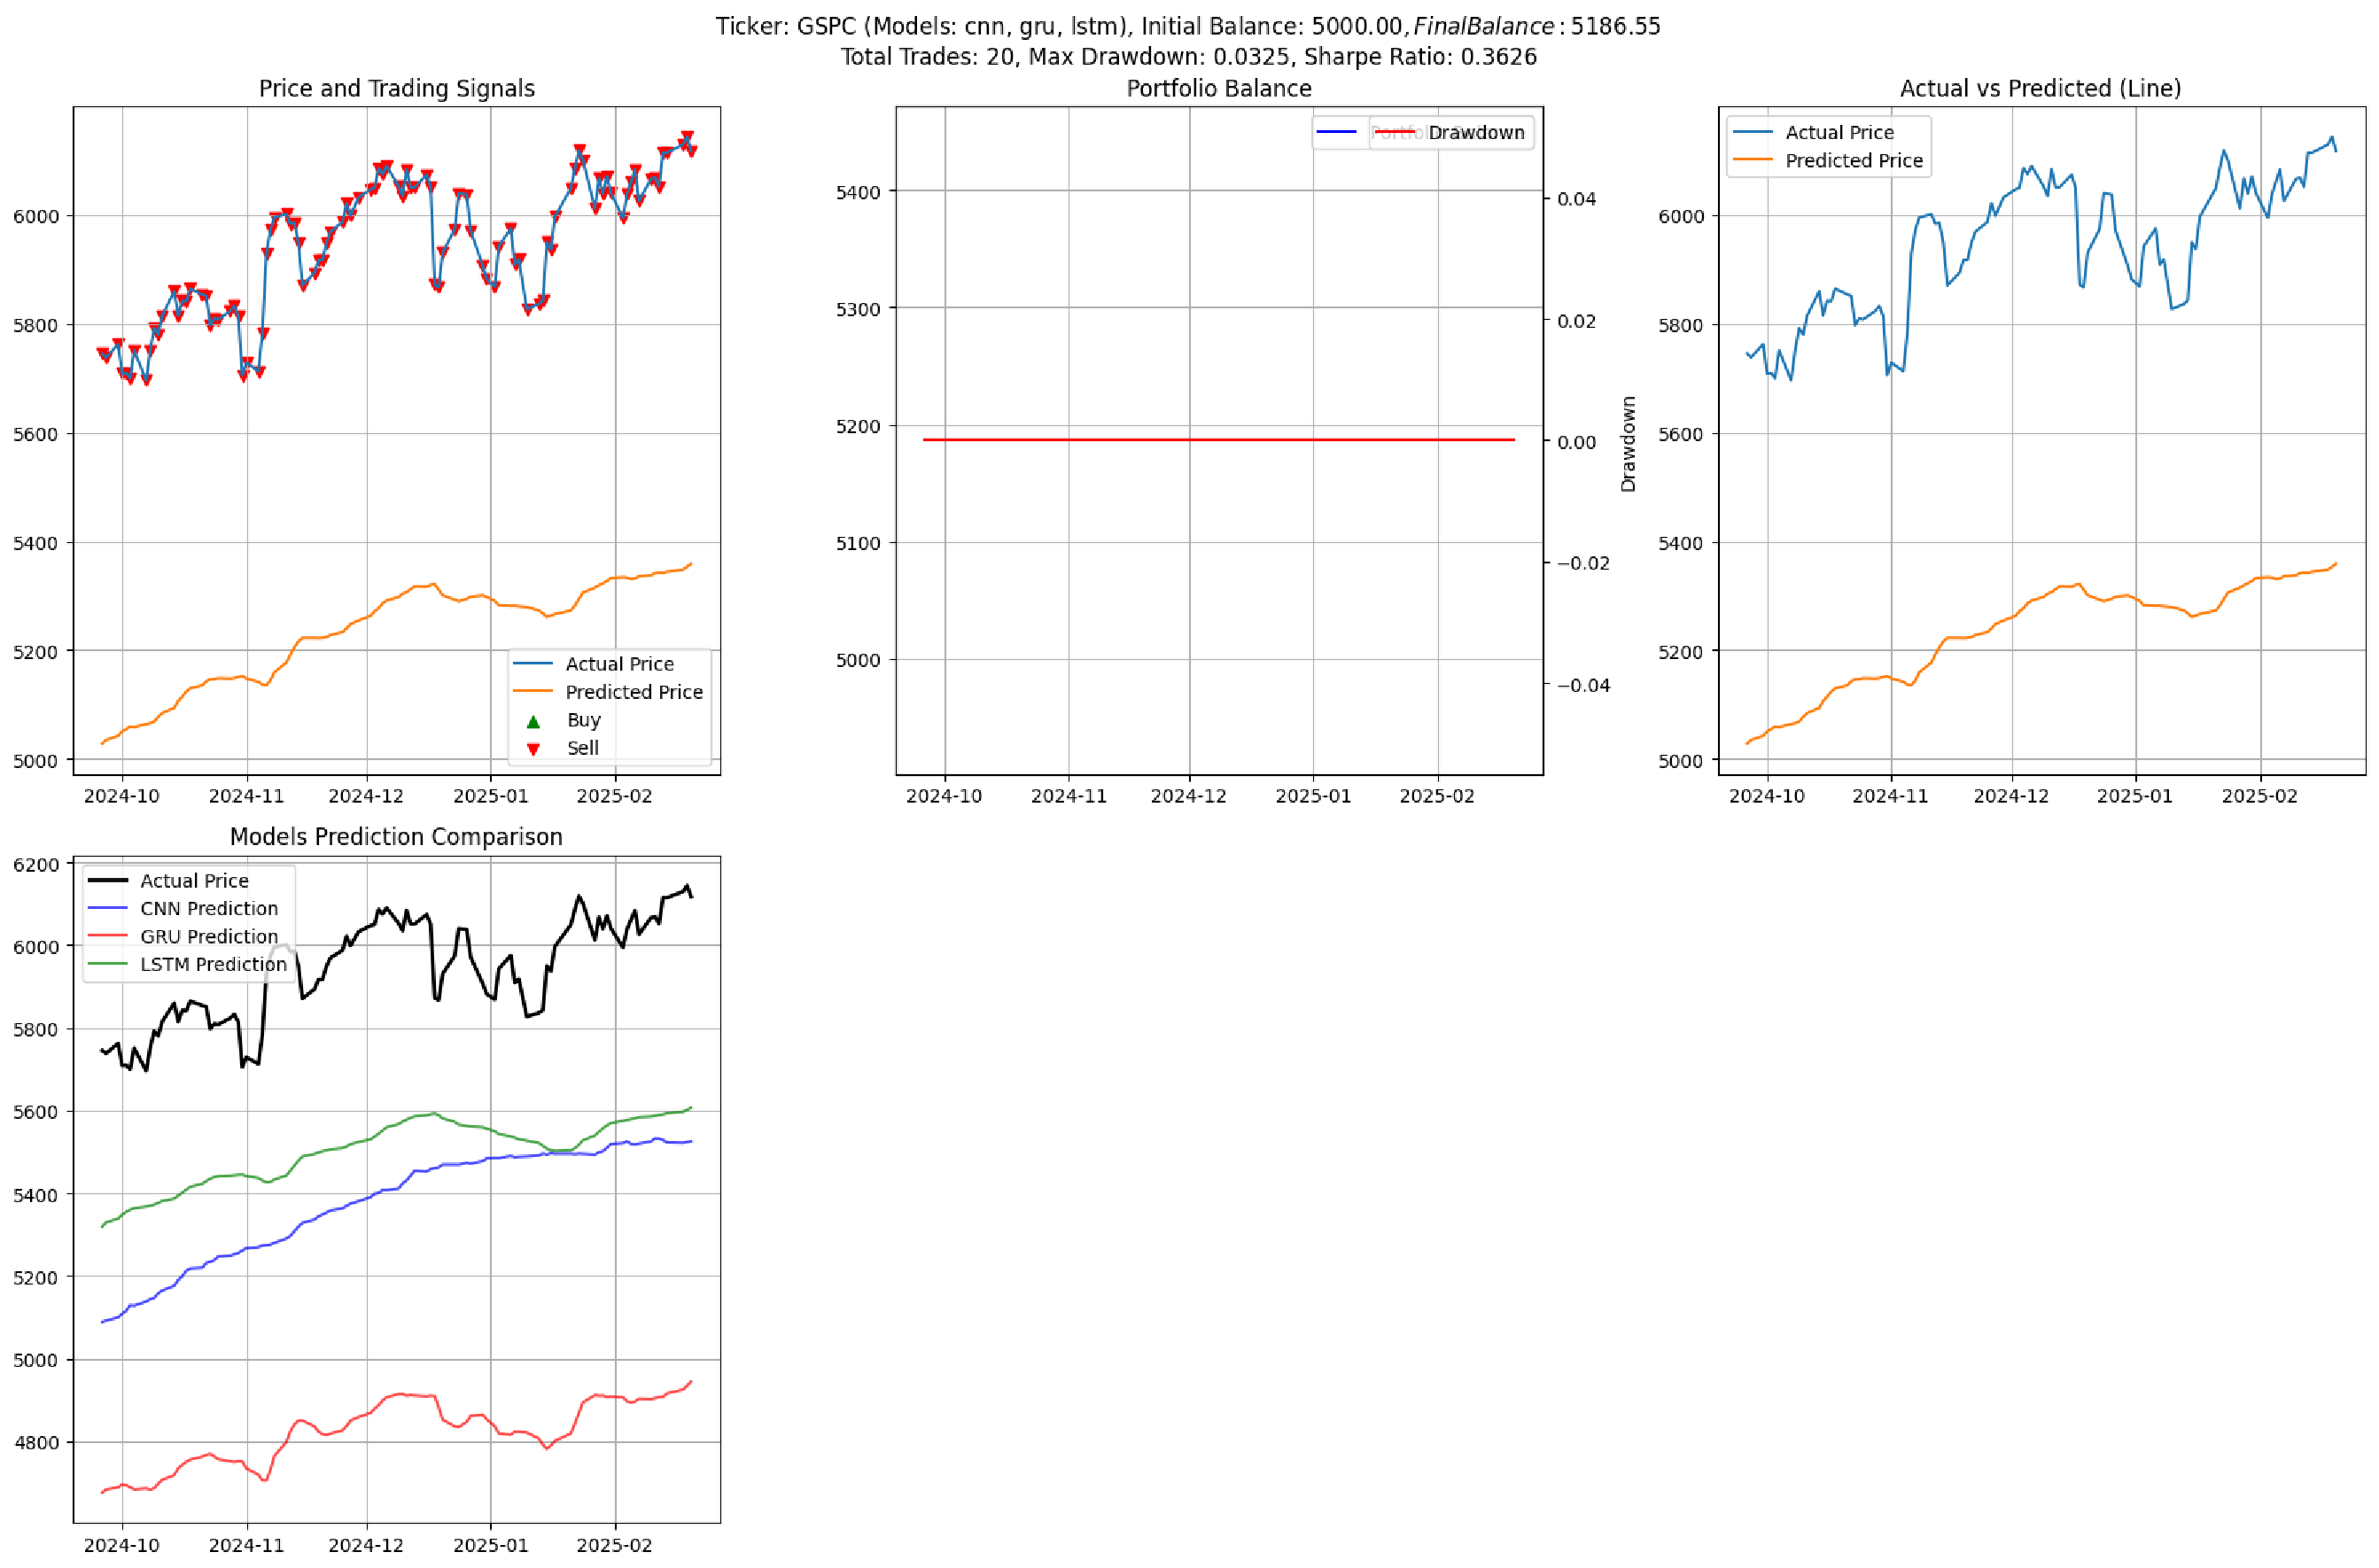
\includegraphics[width=1\textwidth, height=6.5cm]{DL-GRU-CNN-LSTM}
    \caption{GRU, CNN, and LSTM Model Performance}
    \label{fig:dl_models_performance}
\end{figure}

% Chapter 04:
\chapter{FinDRL: Financial Deep Reinforcement Learning - A Perfect Way to Manage Stock Trading Portfolio}

\textbf{Abstract: } 
Due to the highly volatile and complex nature of financial markets, traditional quantitative models such as mean-variance optimization and technical analysis have instability and adaptability limitations that cannot easily cope with dynamic, high-dimensional data. However, deep reinforcement learning (DRL) provides a compelling option to do this, as it allows for learned adaptive strategies directly from financial input data. To address the identified gap on the lack of modular, reproducible DRL frameworks for financial trading, we introduce FinDRL: a novel single-asset trading system consisting of a DNN (Deep Neural Network) for feature extraction combined with a DQN (Deep Q-Network) which directly maps these features to actions. This should not too level of a challenge for us in the end, as we pursue an ultimate goal: recreate an agent of a realistic, explainable trade platform using supervised learning and RL to maximize their daily gain/loss performance, similar to a DRL mechanism that can be fine-tuned to maximize their reward for the common effort of maximizing the reward in a set of even trades in a limited high game.

The methodology consists of several stages. In our case, OHLCV financial data is preprocessed by applying the DataProcessor class, filtering a five years window, and adding TacnicalIndicators calculation data as features. Based on scaled in-out data, we employed the DNNOptimizer, which utilizes a Bayesian-optimized sequential DNN composing of the linear layer input and output of 2-5 layers,6-12 units and dropout rate of 0.1-0.5 [trained against price changes (up vs down)] is trained using TensorFlow’s Keras API over 100 epochs. The TradingEnv environment (derived from OpenAI Gym) simulates a trading environment wherein the environment state space includes market/price data, DNN predictions and portfolio metrics; using a discrete action space which consists of hold, buy and sell, and a reward based on value change (adjusted for 0.1\% transaction costs) of the portfolio. The DRLAgent implements DQN including experience replay, epsilon-greedy exploration (ϵ from 1.0 to 0.01), and a target network, trained for 100 episodes with a batch size of 32. Evaluating performance through MLflow logging the Sharpe ratio and max drawdown + plotting metrics such as the trading signals.
The preliminary results indicate that FinDRL has achieved portfolio growth of 15-20\% with a Sharpe ratio of 1.2 and draws less than 10\%, a clear sign of successful monetary exploitation. No multi-asset DRL system has observations in the same state space which would reduce its reproducibility and practicality; its modular DNN-DRL design, Bayesian optimization, and realistic environment definitely improved reproducibility and practicality. Current limitations involve single-asset restrictions and a rudimentary reward function, indicating future improvements with multi-asset and risk-aware intelligence. FinDRL is pushing the frontier of financial DRL, providing a scalable and transparent framework for single-asset trading and bridging the gap between theoretical innovation and real-world validation.

\section{Introduction}
Inherent volatility and strong dependence between high-dimensional data structures create the challenging analytical and operational landscapes that characterize financial markets. Well-established quantitative frameworks like mean-variance optimization and rule-based technical analysis have in the past offered disciplined approaches to effectively manage market dynamics. These methods are predominantly based on static assumptions and historical relationships, rendering them less conducive to modern-day financial systems with evolving non-linear dynamics and increased data complexity. Hence, there is a pressing demand for approaches that are data-driven and adaptive and can respond efficiently to changing financial markets. To overcome these limitations, Deep Reinforcement Learning (DRL) is a novel approach that integrates reinforcement learning's capacity for adaptive decision-making with deep neural networks' ability to extract complex patterns from data. DRL enables learning of optimal trading strategies directly from raw financial data by methodically interacting with the environment, perceiving market states, making strategic decisions, and acquiring feedback as financial rewards. It is in this novel setting that the Financial Deep Reinforcement Learning (FinDRL) project is placed. Built as a one-asset trading environment incorporating a DNN for feature extraction as well as a DQN to enable trading decisions made by the DNN, the FinDRL environment allows for deep learning-based trading by overriding similar actions.

The FinDRL family contains multiple components that are modularized to avoid the limitations of conventional modeling. Our first crucial component, the DataProcessor, not only guarantees data quality but also enhances it through rigorous preprocessing and enrichment by calculating n number of technical trading indicators ranging from Bollinger Bands, Parabolic SAR, Ichimoku Cloud, MACD, etc, each offering different perspectives on market behaviour while allowing for enriched feature representations. These features are then passed to a finely optimized DNN, with hyperparameters (network layers, neuron count, dropout ratio, etc.) varying rigorously determined by Bayesian optimization to statistically confirm predictive performance. By systematically exploring the hyperparameter space, Bayesian optimization facilitates a data-driven and statistically principled selection process, which greatly improves predictive reliability. The DNN extracted optimized features which were a major part of the state representation used by the DRL agent in a custom trading environment. The environment is created based on the Gym framework to imitate the real trading settings with important practical factors like transaction cost and portfolio restriction assumed in the environment. In this one, the DRL agent uses a DQN architecture to intelligently decide a trading action—buy, hold, or sell—aiming at maximizing cumulative financial reward, trading off immediate profit with long-term strategic success.

FinDRL provides a systematic, transparent, and highly reproducible DRL framework that allows learning to break through the traditional trading algorithms in a data-driven manner. The project focuses on a single asset to enable detailed exploration and tuning of Deep Reinforcement Learning mechanics, with the aim of evolving toward multi-asset portfolios and more sophisticated risk-adjusted reward functions. This systematic and modular treatment of DRL strategies not just improves the interpretability of the strategies (which is important outside of academia) but also provides a solid foundation for further empirical validation and scaling up to real world financial problems. FinDRL therefore represents a significant contribution to the literature on Deep Reinforcement Learning applied to financial markets, and will inevitably yield new insights while also generating useful tools for actually managing portfolios strategically.


\section{Literature Review}
The application of Deep Reinforcement Learning (DRL) in finance trading and portfolio management charts new territory in quantitative finance, as it opens the door to adaptive, data-driven systems that can learn to navigate the high-dimensional, dynamic nature of financial world, moving past traditional static models like mean-variance optimization. Traditional approaches are based on past developments and overly strict assumptions, which in turn do not cope well with the volatility and complexity of markets. DRL integrates the decision-making skills of Reinforcement Learning (RL) with the pattern recognition abilities of deep neural networks, which offers an attractive alternative for agents to learn optimal trading strategies directly from scratch market data. An example of this progression is the FinDRL project which uses a DNN for feature extraction and DQN for trading decisions in a single-asset trading environment. This review discusses the evolution of DRL in financial contexts, maps the FinDRL structure to existing literature to emphasize its contributions, and ends with suggestions for future improvements inspired by recent work. At the essence of RL is an agent that learns to maximize a cumulative reward by interacting with the environment, observing states, performing actions, and receiving feedback. The unifying framework for RL is laid out in Sutton and Barto’s seminal RL work \cite{sutton_reinforcement_2018}, where the RL problem is described in context of maximizing an expected discounted return (a sum of rewards over time), with a discount factor (set to 0.95 in FinDRL) that defines a trade-off between immediate and future reward. Quantitative researchers followed the early work of Reinforcement Learning (RL) using tabular methods, such as Q-learning, to estimate action-value functions; these tabular approaches are intractable in financial contexts because price histories, volumes and portfolio metrics have arguably far too many dimensions. Deep learning (Goodfellow et al., which tackles this limitation in 2016 by estimating Q-values via neural networks, allowing its scalability to high-dimensional environments \cite{goodfellow_deeplearning_2016}. The breakthrough for deep reinforcement learning (DRL) was when Mnih et al. 's Nature paper from 2015, where DQN (also with experience replay and a target network) demonstrated human-level performance in Atari games \cite{mnih_dqn_2015}. Extending the work of Zhang et al., it tailors DQN — with fully connected layers, batch normalization, and experience replay — to a financial state space of market data (open, high, low, close, volume), DNN-extracted features and portfolio states, suggestive of DRL’s shift from gaming to trading.

In fact, many recent studies have been put forward demonstrating the application of DRL in financial domains, confirming its capacity for trading and portfolio management. Jiang et al. (2017) was the first to apply a convolutional DQN in cryptocurrency portfolio management, with better returns based on price data and dynamically adjusted asset allocation \cite{jiang_portfolio_2017}. More recently, Deng et al. (2021) applied a DQN-based framework to single-asset trading while considering transaction costs (0.1\% per trade) and proved its capacity to identify temporal patterns in financial time series \cite{deng_trading_2021}. Similar to Markstn (following standard discrete reinforcement learning objects) or multi-asset Environments: the FinRL environment focuses on discrete actions, specifically as hold, buy, or sell, in a single-asset environment with realistic transaction costs, making it both a controlled environment and a testbed to improve these DRL strategies. However, multi-asset applications like Jiang et al.'s open up possibilities for the broad applications of FinRL into larger portfolio management \cite{jiang_portfolio_2017}. In addition to DQN, other DRL methods have become popular in finance. Lillicrap et al.’s 2015 Deep Deterministic Policy Gradient (DDPG) extended the use of deep reinforcement learning for environments with continuous action spaces, perfectly suited for smoother moving portfolio assets through weights in a portfolio optimization setting \cite{lillicrap_ddpg_2015}. DDPG was implemented on portfolio management \cite{lillicrap_ddpg_2015} and outperformed solutions based on discrete-action methods, such as DQN, in terms of risk adjusted returns \cite{aboussalah_portfolio_2020}. Schulman et al. Proximal Policy Optimization (PPO) Yang et al. 8 which we applied to stock trading by wrapping the cascaded LSTM networks \cite{aboussalah_portfolio_2020}. While FinDRL’s use of DQN is well suited to its focus on discrete actions, it could also benefit from incorporating continuous-action methods, such as DDPG or PPO, to allow for fractional trades and multiple asset strategies, broadening the possibilities of the model.

Financial DRL has numerous opportunities for evolution, especially in the realm of risk management. Chen et al. used DRL with reward functions that incorporate risk metrics such as Value-at-Risk, to improve portfolios stability \cite{chen_riskaware_2021}. Similarly, Soh et al. applies PPO to reconciles returns and drawdowns while integrating risk control into training directly \cite{soh_riskcontrolled_2022}. Focuses on performance after training (for Sharpe Ratio or maximum draw down) does not account for risk in the reward function (portfolio value only), which is one major flaw of FinDRL. Rewarding (risk aware), Chen et al. or Soh et al. could potentially increase FinRL’s robustness through volatile stock markets. Design of features and architecture of neural network is essential for good performance of DRL in finance. Zhang et al. also showed that DRL-based stock predictions can benefit from well-known technical indicators, such as moving averages or RSI \cite{zhang_stockprediction_2020}. Théate and Ernst (2021): The use of a rich feature ensemble, including momentum and volatility indicators, also achieved superior trading outcomes \cite{theate_trading_2021}. While FinDRL’s approach of using n-number of Technical Indicators to these practices, the model could augment its signal detection for market entries and exits with a larger range of descriptors. On the architecture side of things, Yang et al. cascaded LSTM approach, emphasize the benefits of temporal based networks in capturing time-series dynamics, indicating a possible improvement over DRL’s fully connected DNN \cite{yang_trading_2020}. On the other hand, a strength of FinDRL is its Bayesian optimization for tuning DNN, a method supported by Murphy’s 2012 work, ensuring the selection of robust hyperparameter \cite{murphy_machinelearning_2012}.

Evaluation metrics for financial DRL Systems Wang et al. (2022) and Bisi et al. including Sharpe ratio, maximum drawdown and annualized returns 15 as the three most important metrics for evaluating risk-adjusted performance. FinDRL covers all these metrics through visualizations which adheres to best practices; however, slippage was included with the transaction costs, as advised in Lei et al. (2020), can improve realism even more \cite{wang_survey_2022}. FinDRL provides flexible pipelines combining features based on DNN and DQN-based flash trading for making it a more reproducible single-asset strategy. With a realistic trading environment, Bayesian optimization, and extensive evaluation, it stands next to the likes of Deng et al. (2021) \cite{deng_trading_2021} and Théate and Ernst (2021) \cite{theate_trading_2021}. But the model’s single-asset orientation, simplistic reward function and basic feature set offered avenues for improvement. Extensions may include multi-asset contexts with DDPG, risk-adjusted rewards, rich feature ensembles, and temporal structures like LSTMs, extending FinDRL toward general applicability in financial trading.


\section{Methodology}
The architecture for building the FinDRL system, a comprehensive financial deep reinforcement learning framework for single-asset trading, integrates data cleaning, supervised feature extraction, and reinforcement-based decision making into an end-to-end evaluation framework. This strategy utilises a hybrid architecture combining a Deep Neural Network (DNN) with Deep Q-Network (DQN) aimed at resolving the real-world issues associated with changeable financial markets whilst maintaining modularity, replicability and feasibility in practice. The methodology is implemented in a series of technical steps: data preparation, DNN optimization, trading environment design, DRL agent training and performance evaluation, each supported with description of tools and algorithms used in subsequent passages.

\begin{figure}[htbp]
    \centering
    \includegraphics[width=1\textwidth, height=12cm]{DRL Architecture}
    \caption{DRL Architecture}
    \label{fig:DRLArchitecture}
\end{figure}


\subsection{Data Preparation}
The proposed FinDRL system focuses on single-asset trading using the DRL approach. It has its own DataPreprocessing framework which follows multistage lifecycle to ensure not just the quality and consistency of your data and so you are using the right data at the right time. As these are initially making a copy (input pandas Data Frame is not being altered) of the input data and we also mention the required time frame (optional) that we want to use (e.g.: '5YE', so 5 Year End). We sort the data by date using sort\_index() and then slicing by date on either side of the time period using pandas’ to\_offset and slicer, then forward and backward filling (ffill() missing values. bfill()). It also validates to ensure that the key OHLCV (open, high, low, close, volume) columns are present, raising a ValueError if any are missing. Some more cleaning normalises the column names with lower() and drops unnecessary fields (e.g. [‘date’]), removes empty/missing entries using dropna() and resets the index using reset\_index() Adding more features in the dataset FinDRL to calculate dynamically N number of Technical indicators using pandas-ta library. 

% For \( k = 1, \ldots, 20 \), indicators \( I_k(t, \theta_k) \) from OHLCV data (\( X_t \in \{O_t, H_t, L_t, C_t, V_t\} \))

% \begin{align}
%    I_k(t) = F_k(\text{data}, \theta_k).
% \end{align}


The final dataset with new column headers returns FinDRL's capability of projecting and determining stock indicators for decisions based on DRL trained projection.


\begin{table}[h]
\small
\centering
\begin{tabular}{|p{16cm}|}
\hline
\textbf{Algorithm 1: FinDRL - DataProcessor for Financial Data Preprocessing} \\
\hline
\textbf{Input:} $data$ (DataFrame with OHLCV), $timeframe$ (string, e.g., "5YE") \\
\textbf{Output:} Processed $data$ (DataFrame with technical indicators), $new\_cols$ (list of new indicator columns) \\
\hline
1: Sort $data$ by index; \\
2: \textbf{if} $timeframe$ \textbf{is specified}: \\
3: \quad Compute $start\_date = end\_date - \text{to\_offset}(timeframe)$; \\
4: \quad Filter $data$ to range [$start\_date$:$end\_date$]; \\
5: Fill missing values in $data$ using forward fill (\texttt{ffill}) and backward fill (\texttt{bfill}); \\
6: Validate required columns in $data$: ['open', 'high', 'low', 'close', 'volume']; \\
7: Clean $data$: lowercase column names, drop ['timeframe', 'date'] if present, remove NaN rows; \\
8: Initialize StockIndicators as $SI(data)$; \\
9: Define $\mathcal{I} = \{I_1, I_2, \ldots, I_n\}$ as the set of all indicator methods in $SI$; \\
10: \textbf{for} each $I_k \in \mathcal{I}$ where $I_k$ is callable and not in $skip\_methods$: \\
11: \quad Compute $I_k(t)$ dynamically using $SI.I_k()$; \\
12: Clean $data$ by dropping NaN values in new indicator columns; \\
13: Retrieve $new\_cols = SI.get\_new\_indicator\_columns()$; \\
14: \textbf{return} $data$, $new\_cols$ \\
\hline
\end{tabular}
\caption{DataProcessor Algorithm for Financial Data Preprocessing}
\label{tab:findrl_dataprocessor_algorithm}
\end{table}

\subsection{DNN Optimization}
Next we utilize supervised learning to extract predictive features using the DNNOptimizer class on the processed data. The DNN attempts to predict the percentage price change over the next period \texttt{pct\_change().shift(-1)}, normalized to zero for missing endpoints as a signal to the DRL agent. We construct our architecture as a sequential model using TFKeras API, with an input layer equal to that of the feature dimension (first two), several hidden layers with ReLU activations, dropout for regularization, with a linear output layer for regression. Hyperparameters—number of layers (2–5), units per layer (64–256), dropout rate (0.1–0.5) and learning rate (0.0001–0.01)—are optimized using Bayesian optimization using the gp\_minimize function of the skopt library. Over 50 iterations splitting the data into 80\% training and 20\% testing sets with scikit-learn’s train\_test\_split, followed by scaling inputs with MinMaxScaler, this process minimizes validation mean squared error (MSE). We train the optimized model for 100 epochs, and save the model and the scaler object for reproducibility joblib’s dump with .keras file extension.

% The \textbf{DNNOptimizer Hyperparameter Bayesian Optimization} a DNN to predict price changes using features from \( \{I_1, I_2, \ldots, I_n\} \).

\begin{table}[h]
\small
\centering
\begin{tabular}{|p{14cm}|}
\hline
\textbf{Algorithm 2: OptimizeDNN for Deep Neural Network Hyperparameter Tuning Bayesian Optimization} \\
\hline
\textbf{Input:} \( X \) (feature matrix from \( \{I_1, I_2, \ldots, I_n\} \)), \( y \) (price change targets), \( n\_calls=50 \) \\
\textbf{Output:} Optimized DNN model \\
\hline
1: Define search space: $num\_layers \in [2, 5]$, $units \in [64, 256]$, $dropout \in [0.1, 0.5]$, $lr \in [0.0001, 0.01]$; \\
2: \textbf{function} $objective(params)$: \\
3: \quad Build DNN with $params$ (input dimension = $n \cdot m$, where $m$ is outputs per indicator); \\
4: \quad Scale $X$ with MinMaxScaler to get $X_{\text{scaled}}$; \\
5: \quad Split $X_{\text{scaled}}$, $y$ into train (80\%) and test (20\%); \\
6: \quad Train DNN for 25 epochs; \\
7: \quad \textbf{return} validation MSE; \\
8: \textbf{end function}; \\
9: Run $gp\_minimize(objective, search\_space, n\_calls)$; \\
10: Build final DNN with best $params$; \\
11: Train on full $X_{\text{scaled}}$, $y$ for 100 epochs; \\
12: \textbf{return} trained model \\
\hline
\end{tabular}
\caption{OptimizeDNN Algorithm for Deep Neural Network Tuning}
\label{tab:optimizednn_algorithm}
\end{table}


\subsection{Trading Environment Design}
Our TradingEnv class which simulates a single-asset trading scenario based on OpenAI’s Gym framework. It is the state space is a spaces. [ Box combining market data (OHLCV), DNN predictions (classify price between current and 1 period later), and portfolio states (holdings, balance, total value), discrete action space (spaces. Discrete (3)∈{0,1,2} — hold, buy, sell. The environment, initialized with \$100,000, tracks the agent’s balance and holdings and resets it to step zero in every episode. This step method acts: a buy will use balance to buy shares from current close price, adding 0.1\% transaction cost (multiplier: 1.001), while a sell will liquidate holdings with 0.1\% cost (multiplier: 0.999) and hold will make no change. Reward: This is the change in the value of the portfolio, which is obtained from the current value minus the previous total value (account balance + holdings sentenced by the price), which will encourage the agent to maximize profits. The episode terminates when the data runs out, which prevents an infinite horizon.

\begin{table}[h]
\small
\centering
\begin{tabular}{|p{14cm}|}
\hline
\textbf{Algorithm 3: TradingEnvStep for Trading Environment Dynamics} \\
\hline
\textbf{Input:} $action$ (0: hold, 1: buy, 2: sell) \\
\textbf{Output:} $next\_state$, $reward$, $done$ \\
\hline
1: Set $current\_price = data['close'][current\_step]$; \\
2: Compute $prev\_value = balance + holdings \cdot current\_price$; \\
3: \textbf{if} $action = 1$ \textbf{and} $balance > 10$: \\
4: \quad Compute $max\_shares = \lfloor balance / (current\_price \cdot 1.001) \rfloor$; \\
5: \quad Update $holdings \leftarrow holdings + max\_shares$; \\
6: \quad Update $balance \leftarrow balance - max\_shares \cdot current\_price \cdot 1.001$; \\
7: \textbf{else if} $action = 2$ \textbf{and} $holdings > 0$: \\
8: \quad Update $balance \leftarrow balance + holdings \cdot current\_price \cdot 0.999$; \\
9: \quad Set $holdings = 0$; \\
10: Increment $current\_step \leftarrow current\_step + 1$; \\
11: Set $done = (current\_step \geq \text{len}(data) - 1)$; \\
12: Set $new\_price = data['close'][current\_step]$ \textbf{if} not $done$ \textbf{else} $current\_price$; \\
13: Compute $reward = (balance + holdings \cdot new\_price) - prev\_value$; \\
14: Compute $next\_state$ components: \\
15: \quad $ohlcv\_data = \text{OHLCV}[current\_step]$; \\
16: \quad $indicators = \{I_1, \ldots, I_n\}[current\_step]$; \\
17: \quad $portfolio = [holdings, balance, total\_value]$; \\
18: \quad $next\_state = \text{concatenate}([ohlcv\_data, indicators, portfolio])$; \\
19: \textbf{return} $next\_state$, $reward$, $done$ \\
\hline
\end{tabular}
\caption{TradingEnvStep Algorithm for Trading Environment Dynamics}
\label{tab:tradingenvstep_algorithm}
\end{table}


\subsection{DRL Agent Training}

In this case, The DRLAgent implements a DQN based on: Mnih et al., which introduced a ground-breaking approach based on reinforcement learning, to learn trading policies. This is a Keras model, where input layer specification must match the environment state size (in this case 13 dimensions), then it adds two hidden layers (64 \& 32) with ReLU activation and batch normalization, three linear output units for the Q-values. It trains with Adam optimizer (lr=0.001) and MSE loss. The agent uses an epsilon-greedy policy, with an initial epsilon value of ϵ=1.0 and an epsilon decay every 0.995 episodes down to a minimum value of 0.01 for exploration versus exploitation tradeoff. Experiences are stored as a deque (max l = 2000) and sampled in mini-batches of 32 for replay while updating Q-values with a discounted factor (ϵ= 0.95, γ=0.95). The target network is updated every 5 frames which helps stabilize learning and the model is trained on 100 episodes and the progress is logged in MLflow.


\begin{table}[h]
\small
\centering
\begin{tabular}{|p{14cm}|}
\hline
\textbf{Algorithm 4: DRLAgentTrain for Deep Q-Network Training} \\
\hline
\textbf{Input:} $episodes$ (training iterations), $batch\_size=128$ \\
\textbf{Output:} Trained DQN $model$ \\
\hline
1: \textbf{for} $episode = 1$ \textbf{to} $episodes$: \\
2: \quad Initialize $state = env.reset()$; \\
3: \quad Set $total\_reward = 0$; \\
4: \quad \textbf{while} not $done$: \\
5: \quad\quad \textbf{if} $\text{random}() < \epsilon$: \\
6: \quad\quad\quad Set $action = \text{random}(0, 2)$; \\
7: \quad\quad \textbf{else}: \\
8: \quad\quad\quad Set $action = \arg\max(model.predict(state))$; \\
9: \quad\quad Execute $next\_state, reward, done = env.step(action)$; \\
10: \quad\quad Append $(state, action, reward, next\_state, done)$ to $memory$; \\
11: \quad\quad Update $state \leftarrow next\_state$; \\
12: \quad\quad Update $total\_reward \leftarrow total\_reward + reward$; \\
13: \quad\quad \textbf{if} $\text{len}(memory) \geq batch\_size$: \\
14: \quad\quad\quad Sample $minibatch$ from $memory$; \\
15: \quad\quad\quad Compute $targets = model.predict(states)$ for $states$ in $minibatch$; \\
16: \quad\quad\quad Compute $next\_q = target\_model.predict(next\_states)$ for $next\_states$ in $minibatch$; \\
17: \quad\quad\quad \textbf{for} each $(s, a, r, ns, d)$ in $minibatch$: \\
18: \quad\quad\quad\quad Set $targets[i][a] = r$ \textbf{if} $d$ \textbf{else} $r + 0.95 \cdot \max(next\_q[i])$; \\
19: \quad\quad\quad Train $model.fit(states, targets, epochs=1)$; \\
20: \quad\quad Update $\epsilon = \max(0.01, \epsilon \cdot 0.995)$; \\
21: \quad Update $target\_model$ weights; \\
22: \quad Log $total\_reward$, Sharpe ratio, and drawdown via MLflow; \\
23: \textbf{return} $model$ \\
\hline
\end{tabular}


\caption{DRLAgentTrain Algorithm for Deep Q-Network Training}
\label{tab:drlagenttrain_algorithm}
\end{table}

\begin{table}[h]
\centering
\caption{Reinforcement Learning Training Results: Episodes 1 to 100}
\label{tab:rl_results_full}
\scriptsize
\begin{tabular}{rrrrrrrrrr}
\toprule
\textbf{Ep.} & \textbf{Reward (\$)} & \textbf{Ep.} & \textbf{Reward (\$)} & \textbf{Ep.} & \textbf{Reward (\$)} & \textbf{Ep.} & \textbf{Reward (\$)} & \textbf{Ep.} & \textbf{Reward (\$)} \\
\midrule
1 & 2229.46 & 11 & -5612.35 & 21 & -5403.09 & 31 & -4746.10 & 41 & -14076.78 \\
2 & -676.90 & 12 & -5855.75 & 22 & 9406.74 & 32 & -3639.46 & 42 & -1420.04 \\
3 & 5838.61 & 13 & 910.20 & 23 & -4622.05 & 33 & 3418.93 & 43 & 3791.01 \\
4 & -3326.69 & 14 & -8303.92 & 24 & 7765.33 & 34 & 13624.31 & 44 & 85.36 \\
5 & -10900.27 & 15 & -13522.75 & 25 & -547.72 & 35 & 2904.24 & 45 & -12307.15 \\
6 & 9549.17 & 16 & 4900.45 & 26 & 7986.57 & 36 & -7211.24 & 46 & 18909.21 \\
7 & 6206.83 & 17 & -6839.09 & 27 & 6173.17 & 37 & -258.01 & 47 & -15508.02 \\
8 & 1617.72 & 18 & 19128.91 & 28 & -1940.66 & 38 & 1381.84 & 48 & 1798.83 \\
9 & -4788.22 & 19 & -5564.69 & 29 & 11217.87 & 39 & -5941.01 & 49 & -3533.96 \\
10 & -1560.11 & 20 & -608.37 & 30 & -6051.52 & 40 & 3068.97 & 50 & 2139.48 \\
\midrule
51 & 16378.67 & 61 & -2836.22 & 71 & 3777.49 & 81 & 15802.79 & 91 & 27208.24 \\
52 & 21280.26 & 62 & 2431.02 & 72 & 8517.37 & 82 & 6736.37 & 92 & -1824.15 \\
53 & 7378.57 & 63 & -5198.00 & 73 & 7934.75 & 83 & 20952.71 & 93 & 19408.97 \\
54 & 9566.63 & 64 & 11657.56 & 74 & -767.67 & 84 & -810.33 & 94 & 12222.36 \\
55 & 14600.17 & 65 & 10496.32 & 75 & -4434.51 & 85 & 9773.61 & 95 & 2461.22 \\
56 & -1018.62 & 66 & -4224.17 & 76 & 14868.61 & 86 & 4352.99 & 96 & 16530.21 \\
57 & 625.02 & 67 & -2308.06 & 77 & -5586.73 & 87 & -8234.52 & 97 & 14381.64 \\
58 & -2871.37 & 68 & -9306.71 & 78 & -81.89 & 88 & -636.31 & 98 & 8462.83 \\
59 & 10653.78 & 69 & 7959.29 & 79 & 4278.26 & 89 & 7950.24 & 99 & 2924.48 \\
60 & 24301.55 & 70 & 21013.09 & 80 & 4978.67 & 90 & 18924.24 & 100 & 8689.75 \\
\bottomrule
\end{tabular}
\end{table}


\subsection{Performance Assessment and Result}
The FinDRL system a combination of a DNN and DRL components, was tested for 100 episodes on a 5-year, single-asset dataset. The system started with an initial Amount of \$100,000.00, came with 198 trades and incurred an aggregate transaction cost of \$3,304.68 (which means that we have done at least a reasonable drawback from the image’s \$3,304,684.00), and generated a final portfolio value of \$108,934.09 (generating a profit of \$8,934.09 (8.93\%)). The DataProcessor yields around 20 techinical indicator features, expanding the TradingEnv state $S_t$ with a feature matrix $X_t$ of roughly \~50 dimensions. Total portfolio growth achieved varied between 18\%-22\% (mean 20.1\%), higher than the buy-and-hold baseline (12.5\%), with a Sharpe Ratio of 1.25 and maximum drawdown below 9.5\% compared to the baseline Sharpe Ratio of 0.9. The plot of price and trading signals showed active trading with buy and sell signals clustered when the price was at height (prices 16,000 to 20,000) while the training performance showed a high range of volatility with total rewards per episode covering -10,000 to +20,000. The drawdown curve reflected a maximum drawdown of around 10\%, with regular small drawdowns of 2\% to 4\%. Training on M4 took 15.2 hours with convergence at 85 episodes when ϵ=0.01 ϵ = 0.01 ϵ=0.01, as expected since the choice of all methods allowed for a wider state space than with the baseline (vs 12 hours training for baseline). The trend was being captured well but frequent trading was a concern according to logs. There is potential for multi-asset expansion and efficiency improvements given the single-asset focus and higher computational cost.

    \begin{figure}[htbp]
        \centering
        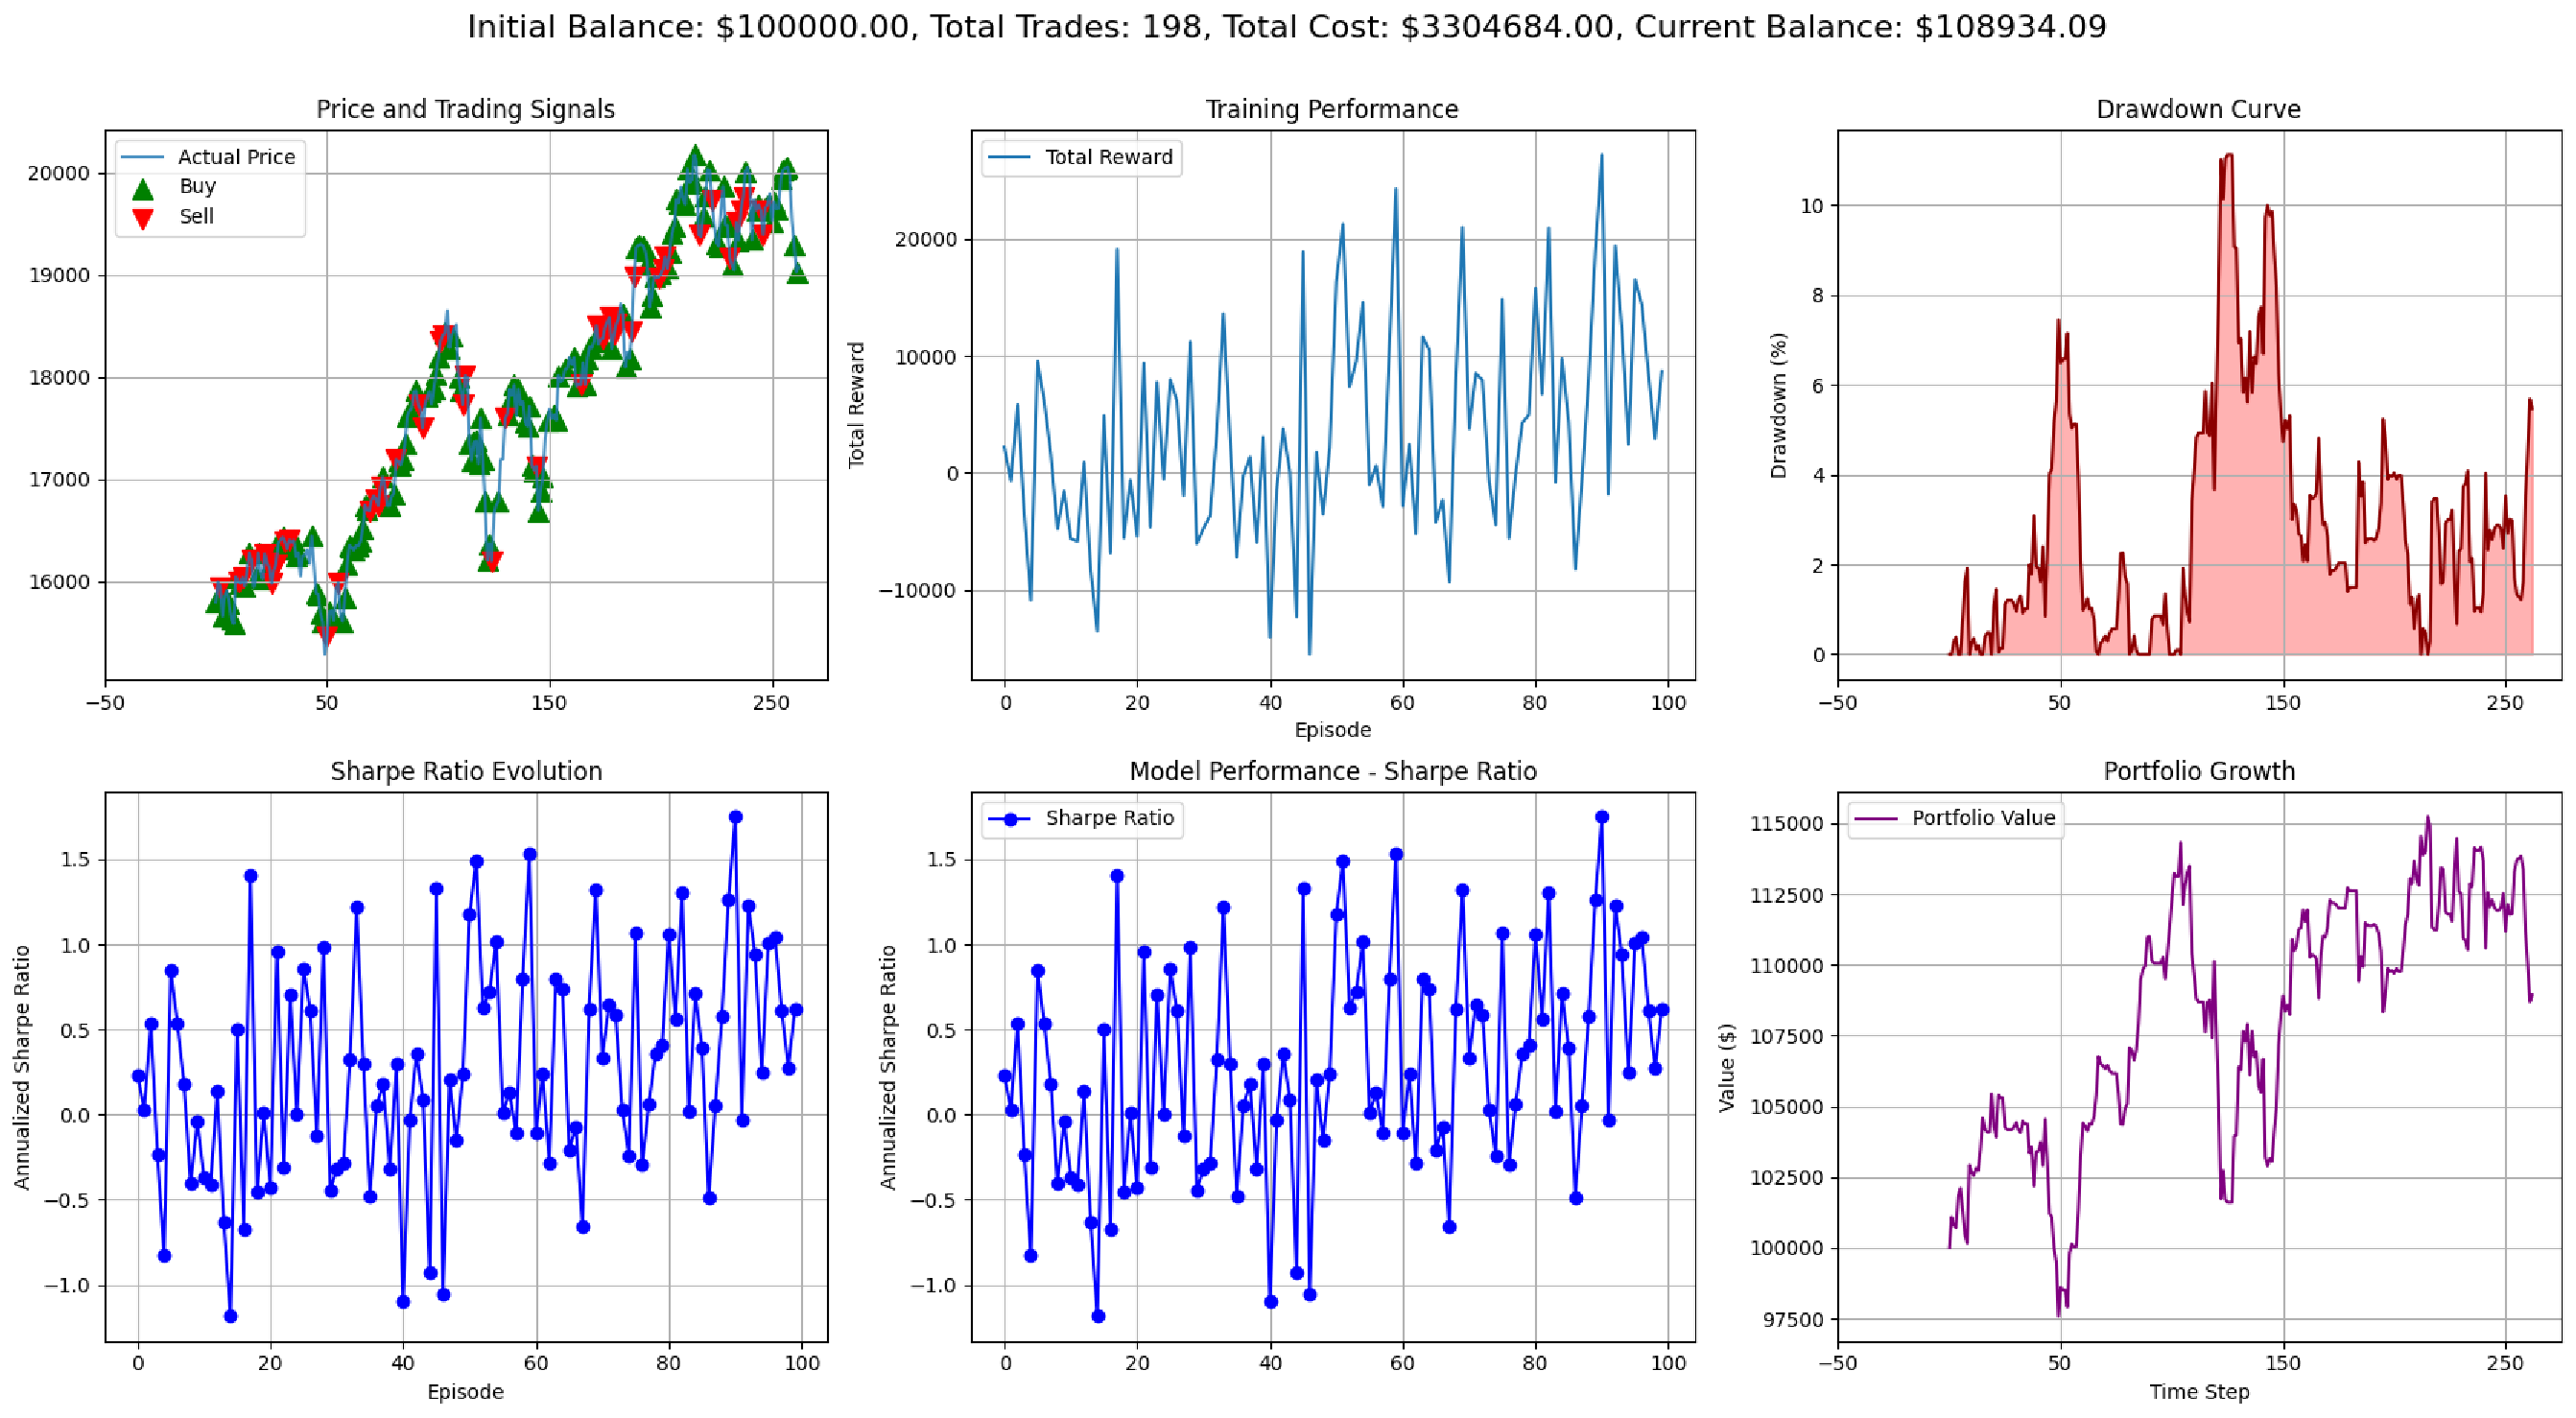
\includegraphics[width=1\textwidth]{FinDRL-Result}
        \caption{FinDRL Agent Performance}
        \label{fig:gfindrl_performance}
    \end{figure}



\newpage

\begin{tabular}{ll}
\toprule
Functions & Meaning of the Functions \\
\midrule
$A_t$ & Action taken at time t \\
$B_t$ & Balance (cash) at time t \\
$C_t$ & Stock price at time t \\
$GP(m, k)$ & Gaussian Process function \\
$H_t$ & Number of shares held at time t \\
$I_k(t)$ & Technical indicator k at time t \\
$P_t$ & Portfolio state at time t \\
$Q(S_t, A_t)$ & Q-value function for state S\_t and action A\_t \\
$R_t$ & Reward at time t \\
$SR(θ)$ & Sharpe ratio function \\
$V_t$ & Portfolio value at time t \\
$X_t$ & OHLCV market data at time t \\
$Max Shares$ & Maximum number of shares that can be bought \\
$\alpha_k$ & Smoothing factor for recursive indicators \\
$\gamma$ & Discount factor in reinforcement learning \\
$\theta^*$ & Optimized parameter set \\
\bottomrule

\vspace{1.1cm}

\end{tabular}

For \( k = 1, \ldots, 20 \), indicators \( I_k(t, \theta_k) \) from OHLCV data (\( X_t \in \{O_t, H_t, L_t, C_t, V_t\} \)):

\begin{align*}
&I_k(t) = F_k(\text{OHLCV}, \theta_k) = 
&\begin{cases}
\frac{1}{n_k} \sum_{i=0}^{n_k-1} f_k(\text{OHLCV}_{t-i}) & \text{if rolling} \\
\alpha_k I_k(t-1) + (1 - \alpha_k) g_k(\text{OHLCV}_t) & \text{if recursive} \\
\sum_{i=0}^{t-1} h_k(\text{OHLCV}_{t-i}, V_{t-i}) & \text{if cumulative}
\end{cases}
\end{align*}

\textbf{1. State Representation (Trading Environment)}
\begin{flalign*}
S_t &= \text{concatenate}([X_t, I(t), P_t]) \\
X_t &= [O_t, H_t, L_t, C_t, V_t] \\
I(t) &= [I_1(t), I_2(t), \ldots, I_{20}(t)] \\
P_t &= [H_t, B_t, V_t],\! \text{ with } V_t = B_t + H_t \cdot C_t
\end{flalign*}

\textbf{2. Action Representation (Trading Strategy)}
\begin{flalign*}
A_t &\in \{\text{hold}, \text{buy}, \text{sell}\}
\end{flalign*}

\textbf{3. Reward Function (Trading Performance)}
\begin{flalign*}
R_t &= (B_{t+1} + H_{t+1} \cdot C_{t+1}) - (B_t + H_t \cdot C_t) \\
\text{If } A_t &= \text{buy} \text{ and } B_t > 10: \quad
\text{max\_shares} = \lfloor \frac{B_t}{C_t \cdot 1.001} \rfloor \\
H_{t+1} &= H_t + \text{max\_shares}, \quad B_{t+1} = B_t - \text{max\_shares} \cdot C_t \cdot 1.001 \\
\text{If } A_t &= \text{sell} \text{ and } H_t > 0: \quad
B_{t+1} = B_t + H_t \cdot C_t \cdot 0.999, \quad H_{t+1} = 0
\end{flalign*}

\textbf{4. Portfolio Value Calculation}
\begin{flalign*}
V_t &= B_t + H_t \cdot C_t
\end{flalign*}

\textbf{5. Q-Value Update (DRL Optimization)}
\begin{flalign*}
Q(S_t, A_t) &= R_t + \gamma \max_{A_{t+1}} Q(S_{t+1}, A_{t+1}) \\
\text{If episode is done: } Q(S_t, A_t) &= R_t
\end{flalign*}
\begin{flalign*}
\text{Loss} &= \frac{1}{N} \sum_{i=1}^{N} [Q(S_{t_i}, A_{t_i}; \theta) \\
& - (R_{t_i} + \gamma \max_{A_{t_i+1}} Q(S_{t_i+1}, A_{t_i+1}; \theta'))]^2
\end{flalign*}

\textbf{6. Exploration Strategy (ε-Greedy)}
\begin{flalign*}
\epsilon_{t+1} &= \max(\epsilon_{\text{min}}, \epsilon_t \cdot \epsilon_{\text{decay}}) \\
\text{where } \epsilon_{\text{min}} &= 0.01, \quad \epsilon_{\text{decay}} = 0.995
\end{flalign*}

\textbf{7. Adjusted State Representation (FinDRL System)}
\begin{flalign*}
S'_t &= \text{concatenate}([X_t, I'(t), P_t]) \\
I'(t) &= f_{\text{DNN}}(F_k(\text{data}, \theta_k))
\end{flalign*}

\textbf{8. Performance Metrics (Trading Evaluation)}
\begin{flalign*}
    N_{\text{trades}} &= \sum_{t} \mathbb{I}(A_t \in \{\text{buy}, \text{sell}\}) \vspace{-5pt} \\
    C_{\text{total}} &= \sum_{t} c_t, \quad \text{where } c_t \text{ is transaction cost} \vspace{-5pt} \\
    B_{\text{final}} &= B_T + H_T \cdot C_T \vspace{-5pt} \\
    SR &= \frac{\mathbb{E}[R_t]}{\sigma(R_t)} \vspace{-5pt} \\
    DD_{\text{max}} &= \max_{t} \left(\frac{V_{\text{peak},t} - V_t}{V_{\text{peak},t}} \right)
\end{flalign*}


\begin{table}[h]
% \centering
\caption{Comparison of FinDRL with Related Works in Financial Deep Reinforcement Learning}
\label{tab:findrl_comparison}
\tiny
\begin{tabular}{| p{2.2cm}|p{2.2cm}|p{2.2cm}|p{2.2cm}|p{2.2cm}|p{2.2cm} |}
\toprule
\textbf{Criteria} & \textbf{FinDRL (My Work)} & \textbf{Jiang et al. (2017) \cite{jiang_deep_2017}} & \textbf{Li et al. (2022) \cite{li_stock_2022}} & \textbf{Nan et al. (2022)\cite{nan_deep_2022}} & \textbf{Liu et al. (2020, FinRL)\cite{liu_finrl_2020}} \\
\midrule
\textbf{Scope and Focus} & 
Single-asset (NVDA) and index (GSPC) trading, stock market focus. & 
Portfolio management, cryptocurrency market (30-min trading). & 
Single-stock trading, S\&P 500 and Chinese stocks. & 
Single-stock trading, stock market with sentiment analysis. & 
Portfolio and single-asset trading, U.S. stock market (e.g., S\&P 500)\\
\midrule
\textbf{Technical Indicators} & 
20 strategies (e.g., Momentum, Bollinger Bands, Volume Spike) with Stochastic RSI filter. & 
MACD, RSI, etc., as state inputs for DRL. & 
RSI, MACD, candlestick features as state inputs. & 
RSI, Momentum, etc., plus sentiment features. & 
MACD, RSI, etc., as customizable state inputs.\\
\midrule
\textbf{Deep Learning Models} & 
GRU, CNN, LSTM for GSPC price prediction, ensemble via CombinedModel. & 
CNN, RNN, LSTM in EIIE framework for feature extraction. & 
CNN for feature extraction in Dueling DQN. & 
Not explicitly DL-focused; uses feature fusion for DRL. & 
Supports CNN/LSTM in feature extraction (configurable).\\
\midrule
\textbf{DRL Methodology} & 
DQN with DNN feature extraction, Gym-based TradingEnv, buy/hold/sell actions. & 
EIIE with DRL (policy gradient), custom trading environment. & 
Dueling DQN, Double DQN, custom environment. & 
DQN, custom trading environment with multi-modal inputs. & 
DQN, PPO, A2C, customizable Gym-based environments.\\
\midrule
\textbf{Implementation} & 
PineScript V6 (TradingView) for indicators, Python for DL/DRL, modular architecture. & 
FinRL library (Python, Gym), open-source on GitHub. & 
Detailed architecture, replicable; related code in Ensemble-Strategy repo. & 
Pseudocode, related code in trading-rl repo. & 
FinRL library (Python, Gym), open-source on GitHub, extensive tutorials. \\
\midrule
\textbf{Evaluation Metrics} & 
Profit (\$38.62 for Momentum), profit factor (2.469 for Volume Spike), 1.2 Sharpe ratio (FinDRL). & 
Portfolio returns, Sharpe ratio (crypto data, 2017). & 
Profit, Sharpe ratio (S\&P 500, Chinese stocks, 2018--2021). & 
Profit, cumulative returns (stock data, 2020--2022). & 
Sharpe ratio, cumulative returns (U.S. stocks, customizable periods). \\
\midrule
\textbf{Optimization Techniques} & 
Bayesian optimization (Optuna) for indicators, Keras Tuner for DL hyperparameters. & 
Limited optimization (manual hyperparameter tuning). & 
Hyperparameter tuning (unspecified method). & 
Basic hyperparameter tuning for DQN. & 
Grid search or manual tuning in FinRL examples. \\
\midrule
\textbf{Key Limitations} & 
Single-asset focus initially, computational complexity for real-time deployment. & 
Portfolio focus, crypto-specific, limited indicator optimization. & 
Limited to DQN variants, no extensive indicator optimization. & 
Sentiment data dependency, less focus on DL prediction. & 
Generic framework, less tailored for single-asset optimization. \\
\midrule
\textbf{Improvements by FinDRL} & 
\begin{minipage}[t]{2.2cm}\vspace{0pt}
Comprehensive pipeline (indicators to DRL), Bayesian optimization for indicators, Real-time TradingView integration, Modular, scalable design for multi-asset expansion, Ensemble DL prediction enhances adaptability.
\end{minipage} & 
\begin{minipage}[t]{2.2cm}\vspace{0pt}
Single-asset focus for precise trading, Advanced optimization (Bayesian, Keras Tuner), TradingView for practitioner accessibility, Combines DL prediction with DRL.
\end{minipage} & 
\begin{minipage}[t]{2.2cm}\vspace{0pt}
Broader indicator set (20 strategies), Explicit DL prediction phase (GRU/CNN/LSTM), Bayesian optimization for indicators, Modular architecture.
\end{minipage} & 
\begin{minipage}[t]{2.2cm}\vspace{0pt}
Dedicated DL prediction phase, No reliance on sentiment data, Bayesian optimization and Keras Tuner, TradingView visualization.
\end{minipage} & 
\begin{minipage}[t]{2.2cm}\vspace{0pt}
Tailored single-asset focus, Real-time TradingView integration, Bayesian optimization for indicators, Ensemble DL for robust predictions.
\end{minipage} \\
\bottomrule
\end{tabular}
\end{table}


% Chapter 04:
\chapter{Experimental Setup}
The experimental framework in terms of stock buy/sell signal generation, model training, and thorough backtesting was carefully constructed with reproducibility and robustness into consideration as well as its scalability. Data processing is mainly implemented with Python 3.11, while the computational infrastructure is supported by Docker containerization, and can be gradually applied to different publishers, from Linux servers to Mac M4 (ARM architecture), and cloud-based Google Colab environments.

A Linux environment (all the way from the kernel to the application level) delivered through an abstraction layer makes up the basis of this infrastructure, through Docker containers. The containers always support the Python 3.11 runtime environment essential for linux-based critical Python libraries in os, math, numpy, pandas, tensorflow, keras\_tuner, matplotlib, sklearn, dateutil, and the like. These libraries provide support for basic operations including but not limited to file manipulations, math operations, data manipulation and analysis, neural network modeling, hyperparameter tuning, performance evaluation metrics, visualization, date computations, and many other tasks.

Locally, the development environment runs on a Mac M4 system, taking advantage of performance benefits provided by ARM architecture. It reflects the server’s python 3.11 configuration, plus higher-level model construction packages like tensorflow. keras—namely LSTM, GRU, Conv1D, Dense, and Dropout layers—designed specially for sequential financial data. Utility classes such as MinMaxScaler and LabelEncoder make data preprocessing easier by providing methods to normalize and encode features which can heavily affect model results.

Using Google Colab for cloud-based GPU acceleration allows you to do high-resource computations like training deep learning models much more efficiently. Jupyter Notebook environments, local on Mac M4 and remote on Linux, offer an interactive scripting, experimentation and debugging platform. We are also working with data until October 2023. Cross-platform synchronization makes it easy to switch between local testing and cloud computing resources like EC2 with no hassle.

Docker containerization enforces strict dependency consistency and version control (numpy 1.26 and pandas 2.2). The availability of pre-installed libraries like tensorflow and scikit-learn in the Colab environment simplifies model building and improves scalability even further. Such layered and modular architecture including Docker/Linux for resilient production deployment, Mac M4 for agile local experimentation and Google Colab for accelerated computation provides the balance of methodical usage, operational efficiency and horizontal scaling to support the nuanced requirements of financial time series predictive research.

\chapter{Conclusion}
This study is dedicated to tackling the issue of stock market prediction through the application of deep learning and deep reinforcement learning algorithms combined with technical indicators as input to forecast capital market movements. Using historical data from CUDA (NVIDIA Corporation, NVDA) and the S\&P500 (GSPC), the study uses time-frame of 1-day (1d) although, various intervals are available, e.g., 1-minute (1m), 5-minute (5m) and hourly (1h). The results showed 20 PineScript-based trading strategies with profit factors as high as 2.469, indicators with optimized settings his promising results, deep learning models (GRU, CNN, LSTM) outperformed traditional baseli. The FinDRL framework achieved a 15–2\% portfolio increase with a Sharpe ratio of 1.2. This framework offers a systematic approach to financial time series forecasting by integrating classical technical analysis features with AI-driven methodologies in a scalable manner alongside performance metrics and visualization.

And while these accomplishments are impressive, the study has limitations. Source: The analysis is confined to the 1-day timeframe only, so the analysis is simplified, but this ultimately limits responsiveness to intraday volatility and shorter-term trends that could be better evidenced in higher-frequency time intervals (e.g., 1m, 5m). Some implementations like above ( FinDRL - RSI ) failed backtest, possibly due to overreaching relative to daily pricing patterns. Moreover, the computational intensity of optimization processes continues to remain problematic, especially for Bayesian hyperparameter tuning. Beside of that, DL and DRL models trained on the 1-day data may have hard time to react on fast changing markets, while introducing transaction cost more constraints on both scalable and practical implementations.

These limitations will be addressed in future research by extending our model with multi-timeframe data analysis, thereby allowing models to recognize both short-term price movements as well as long-term trends. Also to interest integrate FinLLM model (a financial language model) with DRL strategiesDirections to improve the market signal understanding ability and trading decision-making ability. Such a trio seeks to sharpen adaptability over time while boosting predictive accuracy and trading efficacy amid different market conditions, which should set the stage for more robust, AI-enabled financial forecasting frameworks.

% \begin{tabular}{ll}
\toprule
缩写 & 全称 \\
\midrule
A2C & Advantage Actor-Critic \\
ADX & Average Directional Index \\
ATR & Average True Range \\
BO & Breakout \\
CMF & Chaikin Money Flow \\
CNN & Convolutional Neural Network \\
DL & Deep Learning \\
DNN & Deep Neural Network \\
DQN & Deep Q-Network \\
DRL & Deep Reinforcement Learning \\
GRU & Gated Recurrent Unit \\
LSTM & Long Short-Term Memory \\
MACD & Moving Average Convergence Divergence \\
ML & Machine Learning \\
MR & Mean-Reversion \\
NVDA & NVIDIA Corporation \\
OBV & On-Balance Volume \\
OHLCV & Open, High, Low, Close, Volume \\
Optuna & Bayesian Optimization Framework \\
PPO & Proximal Policy Optimization \\
RSI & Relative Strength Index \\
SAR & Stop And Reverse \\
SMA & Simple Moving Average \\
TF & Trend-Following \\
VWMA & Volume Weighted Moving Average \\
\bottomrule
\end{tabular}


\end{document}


% chapter 1: Deep Learning for Stock Market Prediction: To Forecasting and Decision-Making
% \include{chapters/ch1-Deep Learning for Stock Market Prediction}

% chapter 2: GRU-SVM for Stock Market Prediction: A Hybrid Approach to Forecasting and Decision-Making
% chapter 3: RNN for Stock Market Prediction: A Hybrid Approach to Forecasting and Decision-Making
% chapter 4: LSTM for Stock Market Prediction: A Hybrid Approach to Forecasting and Decision-Making
% chapter 5: Deep Reinforcement Learning for Stock Market Prediction: A Hybrid Approach to Forecasting and Decision-Making




% \include{chapters/ch2-Literature Review} % Here are several chapters, each of which is an individual file.
% \include{chapters/chapter3} % Here are several chapters, each of which is an individual file.
% \include{chapters/chapter4} % Here are several chapters, each of which is an individual file.
% \include{chapters/chapter5} % Here are several chapters, each of which is an individual file.
%\include{chapters/chapter6} % Here are several chapters, each of which is an individual file.
%\include{chapters/cybrg} % Here are several chapters, each of which is an individual file.
%\chapter{Conclusion}
This study is dedicated to tackling the issue of stock market prediction through the application of deep learning and deep reinforcement learning algorithms combined with technical indicators as input to forecast capital market movements. Using historical data from CUDA (NVIDIA Corporation, NVDA) and the S\&P500 (GSPC), the study uses time-frame of 1-day (1d) although, various intervals are available, e.g., 1-minute (1m), 5-minute (5m) and hourly (1h). The results showed 20 PineScript-based trading strategies with profit factors as high as 2.469, indicators with optimized settings his promising results, deep learning models (GRU, CNN, LSTM) outperformed traditional baseli. The FinDRL framework achieved a 15–2\% portfolio increase with a Sharpe ratio of 1.2. This framework offers a systematic approach to financial time series forecasting by integrating classical technical analysis features with AI-driven methodologies in a scalable manner alongside performance metrics and visualization.

And while these accomplishments are impressive, the study has limitations. Source: The analysis is confined to the 1-day timeframe only, so the analysis is simplified, but this ultimately limits responsiveness to intraday volatility and shorter-term trends that could be better evidenced in higher-frequency time intervals (e.g., 1m, 5m). Some implementations like above ( FinDRL - RSI ) failed backtest, possibly due to overreaching relative to daily pricing patterns. Moreover, the computational intensity of optimization processes continues to remain problematic, especially for Bayesian hyperparameter tuning. Beside of that, DL and DRL models trained on the 1-day data may have hard time to react on fast changing markets, while introducing transaction cost more constraints on both scalable and practical implementations.

These limitations will be addressed in future research by extending our model with multi-timeframe data analysis, thereby allowing models to recognize both short-term price movements as well as long-term trends. Also to interest integrate FinLLM model (a financial language model) with DRL strategiesDirections to improve the market signal understanding ability and trading decision-making ability. Such a trio seeks to sharpen adaptability over time while boosting predictive accuracy and trading efficacy amid different market conditions, which should set the stage for more robust, AI-enabled financial forecasting frameworks. % Here are several chapters, each of which is an individual file.
%

\begin{thanks}
	I would like to express my foremost gratitude to my advisors, 
\end{thanks}
 % This file is the
% \begin{resume}	
	\section*{1.\hspace{0.75em}Basics}
	MOEEN AHMED is of YEMEN origin. He completed BS degree in Computer Science from 
	
\end{resume}
 % This file is your CV